% Options for packages loaded elsewhere
\PassOptionsToPackage{unicode}{hyperref}
\PassOptionsToPackage{hyphens}{url}
\PassOptionsToPackage{dvipsnames,svgnames*,x11names*}{xcolor}
%
\documentclass[
  12pt,
]{krantz}
\usepackage{amsmath,amssymb}
\usepackage{lmodern}
\usepackage{ifxetex,ifluatex}
\ifnum 0\ifxetex 1\fi\ifluatex 1\fi=0 % if pdftex
  \usepackage[T1]{fontenc}
  \usepackage[utf8]{inputenc}
  \usepackage{textcomp} % provide euro and other symbols
\else % if luatex or xetex
  \usepackage{unicode-math}
  \defaultfontfeatures{Scale=MatchLowercase}
  \defaultfontfeatures[\rmfamily]{Ligatures=TeX,Scale=1}
\fi
% Use upquote if available, for straight quotes in verbatim environments
\IfFileExists{upquote.sty}{\usepackage{upquote}}{}
\IfFileExists{microtype.sty}{% use microtype if available
  \usepackage[]{microtype}
  \UseMicrotypeSet[protrusion]{basicmath} % disable protrusion for tt fonts
}{}
\makeatletter
\@ifundefined{KOMAClassName}{% if non-KOMA class
  \IfFileExists{parskip.sty}{%
    \usepackage{parskip}
  }{% else
    \setlength{\parindent}{0pt}
    \setlength{\parskip}{6pt plus 2pt minus 1pt}}
}{% if KOMA class
  \KOMAoptions{parskip=half}}
\makeatother
\usepackage{xcolor}
\IfFileExists{xurl.sty}{\usepackage{xurl}}{} % add URL line breaks if available
\IfFileExists{bookmark.sty}{\usepackage{bookmark}}{\usepackage{hyperref}}
\hypersetup{
  pdftitle={Bookdown: 使用 R Markdown 创作书籍和技术文档},
  pdfauthor={谢益辉},
  colorlinks=true,
  linkcolor=Maroon,
  filecolor=Maroon,
  citecolor=Blue,
  urlcolor=Blue,
  pdfcreator={LaTeX via pandoc}}
\urlstyle{same} % disable monospaced font for URLs
\usepackage{color}
\usepackage{fancyvrb}
\newcommand{\VerbBar}{|}
\newcommand{\VERB}{\Verb[commandchars=\\\{\}]}
\DefineVerbatimEnvironment{Highlighting}{Verbatim}{commandchars=\\\{\}}
% Add ',fontsize=\small' for more characters per line
\usepackage{framed}
\definecolor{shadecolor}{RGB}{248,248,248}
\newenvironment{Shaded}{\begin{snugshade}}{\end{snugshade}}
\newcommand{\AlertTok}[1]{\textcolor[rgb]{0.94,0.16,0.16}{#1}}
\newcommand{\AnnotationTok}[1]{\textcolor[rgb]{0.56,0.35,0.01}{\textbf{\textit{#1}}}}
\newcommand{\AttributeTok}[1]{\textcolor[rgb]{0.77,0.63,0.00}{#1}}
\newcommand{\BaseNTok}[1]{\textcolor[rgb]{0.00,0.00,0.81}{#1}}
\newcommand{\BuiltInTok}[1]{#1}
\newcommand{\CharTok}[1]{\textcolor[rgb]{0.31,0.60,0.02}{#1}}
\newcommand{\CommentTok}[1]{\textcolor[rgb]{0.56,0.35,0.01}{\textit{#1}}}
\newcommand{\CommentVarTok}[1]{\textcolor[rgb]{0.56,0.35,0.01}{\textbf{\textit{#1}}}}
\newcommand{\ConstantTok}[1]{\textcolor[rgb]{0.00,0.00,0.00}{#1}}
\newcommand{\ControlFlowTok}[1]{\textcolor[rgb]{0.13,0.29,0.53}{\textbf{#1}}}
\newcommand{\DataTypeTok}[1]{\textcolor[rgb]{0.13,0.29,0.53}{#1}}
\newcommand{\DecValTok}[1]{\textcolor[rgb]{0.00,0.00,0.81}{#1}}
\newcommand{\DocumentationTok}[1]{\textcolor[rgb]{0.56,0.35,0.01}{\textbf{\textit{#1}}}}
\newcommand{\ErrorTok}[1]{\textcolor[rgb]{0.64,0.00,0.00}{\textbf{#1}}}
\newcommand{\ExtensionTok}[1]{#1}
\newcommand{\FloatTok}[1]{\textcolor[rgb]{0.00,0.00,0.81}{#1}}
\newcommand{\FunctionTok}[1]{\textcolor[rgb]{0.00,0.00,0.00}{#1}}
\newcommand{\ImportTok}[1]{#1}
\newcommand{\InformationTok}[1]{\textcolor[rgb]{0.56,0.35,0.01}{\textbf{\textit{#1}}}}
\newcommand{\KeywordTok}[1]{\textcolor[rgb]{0.13,0.29,0.53}{\textbf{#1}}}
\newcommand{\NormalTok}[1]{#1}
\newcommand{\OperatorTok}[1]{\textcolor[rgb]{0.81,0.36,0.00}{\textbf{#1}}}
\newcommand{\OtherTok}[1]{\textcolor[rgb]{0.56,0.35,0.01}{#1}}
\newcommand{\PreprocessorTok}[1]{\textcolor[rgb]{0.56,0.35,0.01}{\textit{#1}}}
\newcommand{\RegionMarkerTok}[1]{#1}
\newcommand{\SpecialCharTok}[1]{\textcolor[rgb]{0.00,0.00,0.00}{#1}}
\newcommand{\SpecialStringTok}[1]{\textcolor[rgb]{0.31,0.60,0.02}{#1}}
\newcommand{\StringTok}[1]{\textcolor[rgb]{0.31,0.60,0.02}{#1}}
\newcommand{\VariableTok}[1]{\textcolor[rgb]{0.00,0.00,0.00}{#1}}
\newcommand{\VerbatimStringTok}[1]{\textcolor[rgb]{0.31,0.60,0.02}{#1}}
\newcommand{\WarningTok}[1]{\textcolor[rgb]{0.56,0.35,0.01}{\textbf{\textit{#1}}}}
\usepackage{longtable,booktabs,array}
\usepackage{calc} % for calculating minipage widths
% Correct order of tables after \paragraph or \subparagraph
\usepackage{etoolbox}
\makeatletter
\patchcmd\longtable{\par}{\if@noskipsec\mbox{}\fi\par}{}{}
\makeatother
% Allow footnotes in longtable head/foot
\IfFileExists{footnotehyper.sty}{\usepackage{footnotehyper}}{\usepackage{footnote}}
\makesavenoteenv{longtable}
\usepackage{graphicx}
\makeatletter
\def\maxwidth{\ifdim\Gin@nat@width>\linewidth\linewidth\else\Gin@nat@width\fi}
\def\maxheight{\ifdim\Gin@nat@height>\textheight\textheight\else\Gin@nat@height\fi}
\makeatother
% Scale images if necessary, so that they will not overflow the page
% margins by default, and it is still possible to overwrite the defaults
% using explicit options in \includegraphics[width, height, ...]{}
\setkeys{Gin}{width=\maxwidth,height=\maxheight,keepaspectratio}
% Set default figure placement to htbp
\makeatletter
\def\fps@figure{htbp}
\makeatother
\setlength{\emergencystretch}{3em} % prevent overfull lines
\providecommand{\tightlist}{%
  \setlength{\itemsep}{0pt}\setlength{\parskip}{0pt}}
\setcounter{secnumdepth}{5}
\usepackage{booktabs}
\usepackage{longtable}
\usepackage[bf,singlelinecheck=off]{caption}

\usepackage{Alegreya}
\usepackage[scale=.7]{sourcecodepro}

\usepackage{framed,color}
\definecolor{shadecolor}{RGB}{248,248,248}

\renewcommand{\textfraction}{0.05}
\renewcommand{\topfraction}{0.8}
\renewcommand{\bottomfraction}{0.8}
\renewcommand{\floatpagefraction}{0.75}

\renewenvironment{quote}{\begin{VF}}{\end{VF}}
\let\oldhref\href
\renewcommand{\href}[2]{#2\footnote{\url{#1}}}

\ifxetex
  \usepackage{letltxmacro}
  \setlength{\XeTeXLinkMargin}{1pt}
  \LetLtxMacro\SavedIncludeGraphics\includegraphics
  \def\includegraphics#1#{% #1 catches optional stuff (star/opt. arg.)
    \IncludeGraphicsAux{#1}%
  }%
  \newcommand*{\IncludeGraphicsAux}[2]{%
    \XeTeXLinkBox{%
      \SavedIncludeGraphics#1{#2}%
    }%
  }%
\fi

\makeatletter
\newenvironment{kframe}{%
\medskip{}
\setlength{\fboxsep}{.8em}
 \def\at@end@of@kframe{}%
 \ifinner\ifhmode%
  \def\at@end@of@kframe{\end{minipage}}%
  \begin{minipage}{\columnwidth}%
 \fi\fi%
 \def\FrameCommand##1{\hskip\@totalleftmargin \hskip-\fboxsep
 \colorbox{shadecolor}{##1}\hskip-\fboxsep
     % There is no \\@totalrightmargin, so:
     \hskip-\linewidth \hskip-\@totalleftmargin \hskip\columnwidth}%
 \MakeFramed {\advance\hsize-\width
   \@totalleftmargin\z@ \linewidth\hsize
   \@setminipage}}%
 {\par\unskip\endMakeFramed%
 \at@end@of@kframe}
\makeatother

\makeatletter
\@ifundefined{Shaded}{
}{\renewenvironment{Shaded}{\begin{kframe}}{\end{kframe}}}
\makeatother

\newenvironment{rmdblock}[1]
  {
  \begin{itemize}
  \renewcommand{\labelitemi}{
    \raisebox{-.7\height}[0pt][0pt]{
      {\setkeys{Gin}{width=3em,keepaspectratio}\includegraphics{images/#1}}
    }
  }
  \setlength{\fboxsep}{1em}
  \begin{kframe}
  \item
  }
  {
  \end{kframe}
  \end{itemize}
  }
\newenvironment{rmdnote}
  {\begin{rmdblock}{note}}
  {\end{rmdblock}}
\newenvironment{rmdcaution}
  {\begin{rmdblock}{caution}}
  {\end{rmdblock}}
\newenvironment{rmdimportant}
  {\begin{rmdblock}{important}}
  {\end{rmdblock}}
\newenvironment{rmdtip}
  {\begin{rmdblock}{tip}}
  {\end{rmdblock}}
\newenvironment{rmdwarning}
  {\begin{rmdblock}{warning}}
  {\end{rmdblock}}

\usepackage{makeidx}
\makeindex

\urlstyle{tt}

\usepackage{amsthm}
\makeatletter
\def\thm@space@setup{%
  \thm@preskip=8pt plus 2pt minus 4pt
  \thm@postskip=\thm@preskip
}
\makeatother

\frontmatter
\ifluatex
  \usepackage{selnolig}  % disable illegal ligatures
\fi
\usepackage[]{natbib}
\bibliographystyle{apalike}

\title{Bookdown: 使用 R Markdown 创作书籍和技术文档}
\author{谢益辉}
\date{2021-07-12}

\usepackage{amsthm}
\newtheorem{theorem}{Theorem}[chapter]
\newtheorem{lemma}{Lemma}[chapter]
\newtheorem{corollary}{Corollary}[chapter]
\newtheorem{proposition}{Proposition}[chapter]
\newtheorem{conjecture}{Conjecture}[chapter]
\theoremstyle{definition}
\newtheorem{definition}{Definition}[chapter]
\theoremstyle{definition}
\newtheorem{example}{Example}[chapter]
\theoremstyle{definition}
\newtheorem{exercise}{Exercise}[chapter]
\theoremstyle{definition}
\newtheorem{hypothesis}{Hypothesis}[chapter]
\theoremstyle{remark}
\newtheorem*{remark}{Remark}
\newtheorem*{solution}{Solution}
\begin{document}
\maketitle

%\cleardoublepage\newpage\thispagestyle{empty}\null
%\cleardoublepage\newpage\thispagestyle{empty}\null
%\cleardoublepage\newpage
\thispagestyle{empty}
\begin{center}
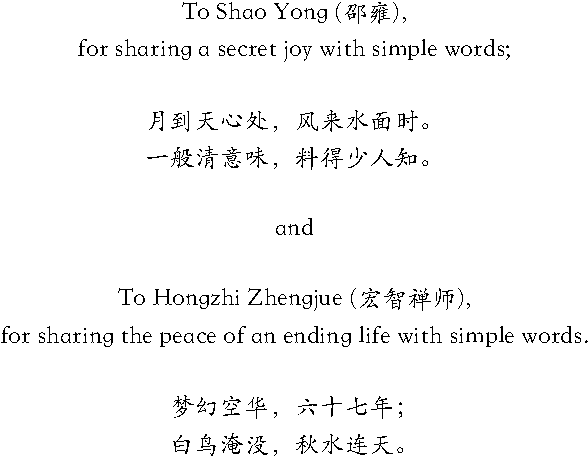
\includegraphics{images/dedication.pdf}
\end{center}

\setlength{\abovedisplayskip}{-5pt}
\setlength{\abovedisplayshortskip}{-5pt}

{
\hypersetup{linkcolor=}
\setcounter{tocdepth}{2}
\tableofcontents
}
\listoftables
\listoffigures
\hypertarget{ux7ffbux8bd1ux4e0eux6392ux7248ux8bf4ux660e}{%
\chapter*{翻译与排版说明}\label{ux7ffbux8bd1ux4e0eux6392ux7248ux8bf4ux660e}}


  本书的简体中文版还没有影子,所以笔者先用自己早就遗忘的文学素养进行翻译,使用与原书相同的技术栈生成中文翻译版本。

\hypertarget{ux7ffbux8bd1ux8bf4ux660e}{%
\section*{翻译说明}\label{ux7ffbux8bd1ux8bf4ux660e}}


  英译中的技术书籍的翻译是个痛苦的过程,难以避免地会遇到一些没有公认翻译方式的英文词汇,或者是有公认的中文翻译词汇,但该词过于口语化,或者不能很好地反映英文词汇的意思。这些英文词汇以及它们在书中的对应中文词汇将在下方列出,欢迎大家批评。

\begin{longtable}[]{@{}
  >{\raggedright\arraybackslash}p{(\columnwidth - 4\tabcolsep) * \real{0.20}}
  >{\raggedright\arraybackslash}p{(\columnwidth - 4\tabcolsep) * \real{0.40}}
  >{\raggedright\arraybackslash}p{(\columnwidth - 4\tabcolsep) * \real{0.40}}@{}}
\toprule
英文词汇 & 中文翻译 & 原因 \\
\midrule
\endhead
package & 软件包,程序包 & r pkgs 是一组用来完成特定任务的程序,作为 R 的补充,符合 Software Package 的定义。 \\
hardcopy & 实体书,书的实体版本 & 原意为``硬拷贝'',指信息被储存并显示在物体实体上,这里采用符合常用语境的翻译。 \\
page margin & 页边空白 & 直译为页面外边距(区域),是页面各边边线离矩形文字区域的垂直距离,四边共同组成了边框形状的区域,通常为空白部分。 \\
typewriter font & 老式打字机字体 & 直译为``打字机字体'',也就是类似于二十世纪七八十年代的铅字打字机的字体,为突出其独特性而强调了``老式'' \\
R plots & (暂无) & (暂无) \\
personal access token & 个人访问令牌 & 参照国内计网教科书对于 token 的翻译进行的直译。 \\
command-line & 命令行(hang,第二声)、命令提示符 & 笔者对于``line''所指的概念不明确,因此参照国内流行的翻译,称为``命令行''。 \\
key & 字段、配置项 & 指的是 YAML 文件中的配置项,位于冒号 \texttt{:} 左侧。由于是``键值对''的形式,因此用了 key 一词,但依照语境翻译为``字段''或是``配置项''。 \\
LaTeX preamble & LaTeX preamble、LaTeX 导言 & 在 \texttt{\textbackslash{}begin\{document\}} 之前的命令称为 ``preamble''(导言),preamble 中通常定义文档的格式、语言等。 \\
Small Capitals & 小型大写字母 & 西文字体设计中的一种字符形式,其大写字母的字高一般与 `x' 等高,并在笔画上做一定的修正,保持更宽的纵横比以保证可读性。 \\
dedication page & 献词页 & 在一些书中,作者想要把这本书献给某人,献词通常写在前几页。 \\
quote & 引用环境(文段) & LaTeX 中的 Quote 环境,放置引用于其他文献中的文段。 \\
copyeditor & 定稿编辑 & 文稿最后付印时按照印刷出版要求进行排版、校正文字和格式错误的编辑。 \\
typeface & 字型 & typeface 与 font 有着微妙的区别,本书中将前者翻译为``字型'',后者翻译为``字体''。且前者多指代印刷用字体。 \\
help desk & 帮助中心 & 直译为``帮助台'',是用来解决用户的 IT 服务问题,降低处置时间的一个服务。 \\
demo & 样例 & 为与 example 区分,demo 翻译为样例,example 翻译为示例。 \\
final words & 结语 & 翻译为中文书籍中常见的``结语''。 \\
index & 主页 & 当描述对象为网页时,翻译为``主页'',指网站的入口点。 \\
in this case & 使用这种方法时 & 将原意``在这种情况下''翻译得更加具体一些。 \\
render & 编译、呈现为、转化为 & 在图形学中一直被翻译为``渲染'',但用在本书中并不合适。考虑到本书中书籍是由源文档\textbf{转化为}多种格式的书籍,其过程涉及源文档的转译(Markdown to LaTeX)与编码,因此翻译为``编译''。另外,它也有``呈现''的意思,在本书中的一些语境下适用。 \\
knit & 生成、``编织'' & 这个词是对于将代码和文字交织在一起的文学编程的形象描述,笔者暂且找不到一个好的词来准确描述该过程,因此使用``生成''或加了双引号的``编织''一词来翻译。 \\
isolate & 剔除 & 作``分离''、``剔除''解释。 \\
side-effects & 副作用 & 这里指程序设计中的``副作用''。如果一个函数修改了自己范围之外的资源,例如读取文件、调用其它有副作用的函数,则该函数称作是有副作用的。 \\
upgrade/update & 升级/更新 & \\
\bottomrule
\end{longtable}

\hypertarget{ux6392ux7248ux8bf4ux660e}{%
\section*{排版说明}\label{ux6392ux7248ux8bf4ux660e}}


  由于书中不可避免地会同时出现中文和英文,因此原书的排版并不完全适用于中文翻译版。为了在尊重原书的基础上使页面变得美观,约定如下排版要求:

\begin{enumerate}
\def\labelenumi{\arabic{enumi}.}
\tightlist
\item
  英文单词、标点符号和数字各具有 1 个前导空格和 1 个后导空格。例如:软件包的名称是 bookdown 吗。

  \begin{itemize}
  \tightlist
  \item
    英文单词、标点和数字的一侧为标点符号时,该侧无空格。例如:使用 Leading and Trailing Spaces。
  \end{itemize}
\item
  需要展示并链接 URL 时,将其放入尖括号内 \texttt{\textless{}\textgreater{}}。
\item
  小括号内的文本包含中文时,使用中文小括号 \texttt{()};如果全是英文文本,则使用英文小括号 \texttt{()},并各具有 1 个前导和后导空格。
\item
  书中某些操作中带有选项、菜单等名称,在实际操作时不具有中文翻译,此时列出该单词的中文翻译,后跟括号,括号内展示原英文单词。中文翻译便于读者查询相关资料,原英文单词便于按图索骥地进行操作。
\end{enumerate}

\hypertarget{ux7ffbux8bd1ux8fdbux5ea6}{%
\section*{翻译进度}\label{ux7ffbux8bd1ux8fdbux5ea6}}


  常言道,人生未填之坑十之八九。笔者学业繁忙,只能利用空闲时间翻译本书。因此在这里记录一下翻译进度,欢迎加入本项目提交 Pull Request。

\begin{longtable}[]{@{}ccc@{}}
\toprule
章节 & 是否翻译 & 是否润色 \\
\midrule
\endhead
preface & √ & × \\
Author & √ & × \\
Introduction & √ & × \\
Components & × & × \\
Output Formats & × & × \\
Customization & × & × \\
Editing & × & × \\
Publishing & √ & × \\
Appendix & × & × \\
References & √ & × \\
\bottomrule
\end{longtable}

\hypertarget{ux524dux8a00}{%
\chapter*{前言}\label{ux524dux8a00}}


  这本短小精悍的书籍介绍了一个 R 软件包 \textbf{bookdown},它能够改变你创作书籍的流程。写一本书在技术上要容易,看书时在视觉上要舒适愉悦,与书互动时要有趣,总览全书要方便,读者能够直截了当地为书籍内容做出贡献,或是给作者留下反馈。最重要的是,作者不应该总是被排版细节分散注意力。

  \textbf{Bookdown} 是构建在 R Markdown (\url{http://rmarkdown.rstudio.com}) 之上的一个拓展包,它继承了 Markdown 语法的简单性(你能够在5分钟内学会基础内容;请看第 \ref{markdown-syntax} 节),同时也继承了以多种格式 (PDF/HTML/Word/\ldots) 进行输出的可能性。同时,它添加了多页HTML输出、图/表/节/方程的编号与交叉引用、插入多章组成的部分/附录等功能,并导入了 GitBook\index{GitBook} 样式 (\url{https://www.gitbook.com}) 以创建优雅迷人的HTML书页。这本书本身就是一个教你如何从一系列 R Markdown 文档中生成一本书籍的例子,并且其印刷版与在线版都能够有专业的观感。你能够在 \url{https://bookdown.org} 上找到更多的例子。

  尽管名称中包含了``Book''一词,但 \textbf{Bookdown} 软件包并不仅仅适用于写书。``书''可以是任何能够按照线性顺序阅读的一系列 R Markdown 文档,例如课程讲义、学习笔记、软件使用手册、论文,甚至可以是日记。事实上,许多 \textbf{bookdown} 特性也适用于单个 R Markdown 文档(请见第 \ref{a-single-document} 节)。


\includegraphics{images/by-nc-sa.png}\\
本书的在线版本依据 \href{http://creativecommons.org/licenses/by-nc-sa/4.0/}{Creative Commons Attribution-NonCommercial-ShareAlike 4.0 International License} 许可证进行授权。另外,你能够在 \href{https://www.crcpress.com/product/isbn/9781138700109}{Chapman \& Hall} 或者亚马逊上购买本书的实体版本。

\hypertarget{ux4e3aux4ec0ux4e48ux8981ux9605ux8bfbux8fd9ux672cux4e66}{%
\section*{为什么要阅读这本书}\label{ux4e3aux4ec0ux4e48ux8981ux9605ux8bfbux8fd9ux672cux4e66}}


  我们能够只使用一种源文档格式编写书籍,但能生成多种格式的输出文档吗?书籍传统上通常是使用 LaTeX 或者 Microsoft Word 进行编写的。但不论是哪种工具都会使得写书变成一趟单程旅行,你无法回头:如果选择 LaTeX,你通常只会得到一个 PDF 文档;如果使用 Word,你可能不得不永远挣扎在 Word 的泥潭中,而且可能会错过许多有用的特性以及来自 LaTeX 的漂亮的 PDF 输出。

  我们能够专注于书写内容而不用太担心排版吗?内容和外观之间似乎有着天然的矛盾,我们总是要平衡花费在这两方面上的时间。鱼和熊掌不可兼得,但这并不意味着我们不能吃到半条鱼和半块熊掌。我们希望我们的书看起来美观,我们也希望把注意力集中在内容上。一种选择是暂时放弃 PDF 输出,作为回报,你可能会得到一个相当不错的HTML网页\index{HTML}预览版。LaTeX\index{LaTeX} 是一个非常好的排版工具,但是在编写书籍的过程中,你很容易沉浸于大量的 LaTeX 命令和排版细节。我们很难避免通过 PDF 预览正在编写的书籍,然而不幸的是,我们经常会发现某些单词超出了页边空白,某些图片浮动到随机的页面上,一章末尾的五到六个零星的单词骄傲地占据了一个全新的页面\ldots\ldots 如果书籍要印刷,我们最终将不得不处理这些问题,但当你在创作书的内容时,不值得一次又一次为此分心。事实上,Markdown 语法比 LaTeX 更加简单,功能更少,这有助于你专注于书的内容。真的有必要自己定义一个像 \texttt{\textbackslash{}myprecious\{\}} 一样的新命令来将 \texttt{\textbackslash{}textbf\{\textbackslash{}textit\{\textbackslash{}textsf\{\}\}\}} 应用到文本上吗?当读者能够轻易地理解字母``R''代表 R 语言时,字母``R''是否有必要包括在 \texttt{\textbackslash{}proglang\{\}} 中?如果读者需要关注书籍的每一处细节,那这和读者什么都不关注有什么区别呢?因此好的书籍创作技术应该帮助作者自动解决对于内容不重要的细节,让作者关注重点内容。

  读者能和我们的书籍中的例子进行互动吗?如果书籍是打印在纸上的,答案当然是不能。但如果你的书籍有 HTML 版本,并包含了在线示例,例如 Shiny 应用 (\url{https://shiny.rstudio.com}) 或 HTML 组件 (\url{https://htmlwidgets.org}),那么读者阅读时就可能能够与书进行互动。例如,读者能够立刻知道如果他们改变了统计模型的某些参数后会发生什么。

  我们能够在创作书籍时得到来自读者的反馈,甚至是内容贡献吗?传统上,编辑会找一小部分匿名评审员来审查你的书。评审员往往很有帮助,但你仍然可能错过来自更有代表性的读者的智慧。如果读者只有等到第一版印刷发布之后才能够看到你的书,那可能已经太迟了,他们可能需要等待好几年才能看到增订修改后的第二版。有一些网络平台,人们可以轻松地利用它们提供反馈并为你的项目做出贡献。GitHub (\url{https://github.com}) 就是一个突出的例子。如果有人在你的书里发现一个拼写错误,他/她能够简单地进行在线更正,并将更改提交给你供你审阅批准。你只需要点击一个按钮来合并更改,无需询问任何问题或来回发送邮件。为了能够使用这些平台,你需要学习 GIT 等版本控制系统,并且你的书籍源文件应该是纯文本。

  R (\url{https://www.r-project.org})、Markdown 和 Pandoc (\url{http://pandoc.org}) 的组合使得将文档从一种简单的源格式 (R Markdown) 转换为多种格式(PDF、HTML、EPUB 和 Word\ldots\ldots)成为可能。\textbf{bookdown} 软件包的功能基于 R Markdown 实现,并为书籍和长篇文章提供输出格式,其中包括 GitBook 格式,它是一种多页面 HTML 输出格式,有着实用且美观的用户界面。用 HTML 进行排版比用 LaTeX 轻松得多,因此你能够经常使用 HTML 预览你的书籍,并且在内容基本完成后再转为 PDF 进行调整。可运行示例很容易就能够插入 HTML 中,它可以使得书籍更具有吸引力和实用性。R Markdown 是一种纯文本格式,因此你也能享受版本控制的优势,例如在 GitHub 上协作创作。我们还努力将一些重要特性从 LaTeX 移植到 HTML 和其它输出格式上,例如图/表编号和交叉引用。

  简单来说,你只需要准备一些 R Markdown 格式的书籍章节文档,然后 \textbf{bookdown} 就能帮助你将它们转变成一本漂亮的书。

\hypertarget{ux672cux4e66ux7684ux7ed3ux6784}{%
\section*{本书的结构}\label{ux672cux4e66ux7684ux7ed3ux6784}}


  第 \ref{introduction} 和 \ref{components} 章介绍了基础用法和语法,对大多数读者来说应该足够让他们开始创作书籍。第 \ref{output-formats} 和 \ref{customization} 章是为了那些想要微调书籍外观的读者准备的。如果你不熟悉 HTML/CSS 和 LaTeX,这部分内容可能看起来很技术化。当你第一次阅读本书时,不必非常仔细地阅读这两章。你可以先学习书籍外观的哪些部分可以被改变,之后再回来了解它们是如何被改变的。对于第 \ref{editing} 章,里面的技术细节并不重要,除非你不使用 RStudio IDE(第 \ref{rstudio-ide} 节)。同样地,你可能会对第 \ref{publishing} 章中用于发布书籍的命令感到不知所措,但我们仍然可以通过 RStudio IDE 简化你在线发布书籍的流程。自定义命令和函数仅适用于那些选择不使用 RStudio 的服务或想要明白技术细节的读者。

  综上所述,本书是对 \textbf{bookdown} 程序包的综合参考书。你在阅读时可以遵循 \href{https://en.wikipedia.org/wiki/Pareto_principle}{80/20 法则}。有些章节的存在是为了内容的完整性,并不是所有章节都对你想写的书同样有用。

\hypertarget{ux8f6fux4ef6ux4fe1ux606fux4e0eux4e00ux4e9bux7ea6ux5b9a}{%
\section*{软件信息与一些约定}\label{ux8f6fux4ef6ux4fe1ux606fux4e0eux4e00ux4e9bux7ea6ux5b9a}}


  本书内容主要关于 R 的软件包 \textbf{bookdown},因此你至少需要安装 R 和 \textbf{bookdown} 软件包。不过,你的书籍根本不必与 R 语言相关。你可以使用其它计算语言(C++、SQL、Python 等;详情请见附录 \ref{software-usage}),甚至可以与计算完全无关(例如,你可以创作小说或者是诗集)。附录 \ref{software-tools} 介绍了创作并构建一本书籍所需的软件工具。

  编译本书时的 R Session 信息如下所示:

\begin{Shaded}
\begin{Highlighting}[]
\FunctionTok{sessionInfo}\NormalTok{()}
\end{Highlighting}
\end{Shaded}

\begin{verbatim}
## R version 4.0.3 (2020-10-10)
## Platform: x86_64-w64-mingw32/x64 (64-bit)
## Running under: Windows 10 x64 (build 19042)
## 
## Matrix products: default
## 
## locale:
## [1] LC_COLLATE=Chinese (Simplified)_China.936 
## [2] LC_CTYPE=Chinese (Simplified)_China.936   
## [3] LC_MONETARY=Chinese (Simplified)_China.936
## [4] LC_NUMERIC=C                              
## [5] LC_TIME=Chinese (Simplified)_China.936    
## 
## attached base packages:
## [1] stats     graphics  grDevices utils     datasets 
## [6] methods   base     
## 
## loaded via a namespace (and not attached):
## [1] bookdown_0.22     miniUI_0.1.1.1   
## [3] rmarkdown_2.9     tools_4.0.3      
## [5] shiny_1.6.0       htmltools_0.5.1.1
## [7] knitr_1.33
\end{verbatim}

  我们在本书的源代码中没有添加提示符(\texttt{\textgreater{}} 和 \texttt{+}),默认情况下我们使用两个 \texttt{\#\#} 标签注释掉文本输出,就像你在上面的 R Session 信息中看到的那样。这样做是为了让你能够方便地复制和运行代码(由于文本输出被注释掉了,因此执行代码时会被忽略)。程序包名称以粗体显示(例如,\textbf{rmarkdown}),行内代码和文件名用老式打字机字体进行格式化(例如,\texttt{knitr::knit(\textquotesingle{}foo.Rmd\textquotesingle{})})。函数名称后跟括号(例如,\texttt{bookdown::render\_book()})。双冒号操作符 \texttt{::} 表示从软件包的命名空间对其中的对象进行访问。

\hypertarget{ux81f4ux8c22}{%
\section*{致谢}\label{ux81f4ux8c22}}


First I'd like to thank my employer, RStudio, for providing me the opportunity to work on this exciting project. I was hoping to work on it when I first saw the GitBook project in 2013, because I immediately realized it was a beautiful book style and there was a lot more power we could add to it, judging from my experience of writing the \textbf{knitr} book \citep{xie2015} and reading other books. R Markdown became mature after two years, and luckily, \textbf{bookdown} became my official job in late 2015. There are not many things in the world better than the fact that your job happens to be your hobby (or vice versa). I totally enjoyed messing around with JavaScript libraries, LaTeX packages, and endless regular expressions in R. Honestly I should also thank Stack Overflow (\url{https://stackoverflow.com}), and I believe you all know \href{http://bit.ly/2cWbiAp}{what I mean,} if you have ever written any program code.

This project is certainly not a single person's effort. Several colleagues at RStudio have helped me along the way. Hadley Wickham provided a huge amount of feedback during the development of \textbf{bookdown}, as he was working on his book \emph{R for Data Science} with Garrett Grolemund. JJ Allaire and Jonathan McPherson provided a lot of technical help directly to this package as well as support in the RStudio IDE. Jeff Allen, Chaita Chaudhari, and the RStudio Connect team have been maintaining the \url{https://bookdown.org} website. Robby Shaver designed a nice cover image for this book. Both Hadley Wickham and Mine Cetinkaya-Rundel reviewed the manuscript and gave me a lot of helpful comments. Tareef Kawaf tried his best to help me become a professional software engineer. It is such a blessing to work in this company with enthusiastic and smart people. I remember once I told Jonathan, ``hey I found a problem in caching HTML widgets dependencies and finally figured out a possible solution''. Jonathan grabbed his beer and said, ``I already solved it.'' ``Oh, nice, nice.''

I also received a lot of feedback from book authors outside RStudio, including Jan de Leeuw, Jenny Bryan, Dean Attali, Rafael Irizarry, Michael Love, Roger Peng, Andrew Clark, and so on. Some users also contributed code to the project and helped revise the book. Here is a list of all contributors: \url{https://github.com/rstudio/bookdown/graphs/contributors}. It feels good when you invent a tool and realize you are also the beneficiary of your own tool. As someone who loves the GitHub pull request model, I wished readers did not have to email me there was a typo or obvious mistake in my book, but could just fix it via a pull request. This was made possible in \textbf{bookdown}. You can see how many pull requests on typos I have merged: \url{https://github.com/rstudio/bookdown/pulls}. It is nice to have so many outsourced careful human spell checkers. It is not that I do not know how to use a real spell checker, but I do not want to do this before the book is finished, and the evil Yihui also wants to leave a few simple tasks to the readers to engage them in improving the book.

Callum Webb kindly designed a nice hexbin sticker for \textbf{bookdown}.

The \textbf{bookdown} package is not possible without a few open-source software packages. In particular, Pandoc, GitBook, jQuery, and the dependent R packages, not to mention R itself. I thank the developers of these packages.

I moved to Omaha, Nebraska, in 2015, and enjoyed one year at Steeplechase Apartments, where I lived comfortably while developing the \textbf{bookdown} package, thanks to the extremely friendly and helpful staff. Then I met a professional and smart realtor, Kevin Schaben, who found a fabulous home for us in an amazingly short period of time, and I finished this book in our new home.

John Kimmel, the editor from Chapman \& Hall/CRC, helped me publish my first book. It is my pleasure to work with him again. He generously agreed to let me keep the online version of this book for free, so I can continue to update it after it is printed and published (i.e., you do not have to wait for years for the second edition to correct mistakes and introduce new features). I wish I could be as open-minded as he is when I'm his age. Rebecca Condit and Suzanne Lassandro proofread the manuscript, and their suggestions were professional and helpful. Shashi Kumar solved some of my technical issues with the publisher's LaTeX class (\texttt{krantz.cls}) when I was trying to integrate it with \textbf{bookdown}. I also appreciate the very helpful comments from the reviewers Jan de Leeuw, Karl Broman, Brooke Anderson, Michael Grayling, Daniel Kaplan, and Max Kuhn.

Lastly I want to thank my family, in particular, my wife and son, for their support. The one-year-old has discovered that my monitor will light up when he touches my keyboard, so occasionally he just creeps into my office and presses randomly on the keyboard when I'm away. I'm not sure if this counts as his contribution to the book\ldots{} @)!\%)\&@*

\begin{flushright}
Yihui Xie\\
Elkhorn, Nebraska
\end{flushright}

\hypertarget{ux5173ux4e8eux4f5cux8005}{%
\chapter*{关于作者}\label{ux5173ux4e8eux4f5cux8005}}


  谢益辉 (\url{http://yihui.org}) 是 RStudio 的软件工程师 (\url{http://www.rstudio.com})。 他在爱荷华州立大学统计系获得了博士学位。他对交互式统计图形和统计计算感兴趣。作为一个活跃的 R 语言用户,他编写了多个 R 包,如 \textbf{knitr}、\textbf{bookdown}、\textbf{blogdown}、\textbf{animation}、\textbf{DT}、\textbf{tinytex}、\textbf{tufte}、\textbf{formatR}、\textbf{fun}、\textbf{mime}、\textbf{highr}、\textbf{servr}、\textbf{Rd2roxygen} 等,其中 \textbf{animation} 软件包荣获 2009 年的 John M. Chambers Statistical Software Award (ASA)。他还与人合著了其他一些 R 软件包,包括 \textbf{shiny}、\textbf{rmarkdown} 和 \textbf{sliple}。

  2006 年,他创立了统计之都 (\url{https://cosx.org}),它已经发展成为中国的一个大型统计网络社区。他于 2008 年发起了中国 R 语言会议,并从那时起参与了在中国组织 R 语言会议。在爱荷华州立大学攻读博士学位期间,他获得了 Vince Sposito Statistical Computing Award (2011) 和统计部的 Snedecor Award (2012)。

  他偶尔在推特上咆哮 (\url{https://twitter.com/xieyihui}),大多数时候你都可以在 GitHub 上找到他 (\url{https://github.com/yihui}).

  他喜欢中国古典文学,同样喜欢辛辣的食物。

\mainmatter

\hypertarget{introduction}{%
\chapter{简介}\label{introduction}}

  这本书是使用 R Markdown \citep{R-rmarkdown} 和 R 软件包 \textbf{bookdown} \citep{R-bookdown} 创作书籍和技术文档的指南。它侧重于创作书籍、长篇文章或报告所需要使用的功能,例如:

\begin{itemize}
\tightlist
\item
  公式、定理、图表的排版和交叉引用;
\item
  如何为一本书生成多种输出格式,例如 HTML、PDF 和电子书;
\item
  怎样自定义书本模板并为书中不同元素设置样式;
\item
  编辑器支持(尤其是 RStudio IDE);
\item
  怎样发布书籍;
\end{itemize}

  这不是对 R Markdown 或 \textbf{knitr} 软件包\citep{R-knitr}的全面介绍,尽管 \textbf{bookdown} 就是在这个软件包的基础上构建的。要了解有关 R Markdown 的更多信息,请查看联机文档 \url{http://rmarkdown.rstudio.com}。关于 \textbf{knitr},请参阅 \citet{xie2015}。你不必是 R 语言\citep{R-base}的专家就可以阅读这本书,但是你应该对 R Markdown 和 \textbf{knitr} 有一些基本的了解。对于初学者,你可以从 \url{https://www.rstudio.com/resources/cheatsheets/} 上的备忘单开始学习。本书的附录包含对这些软件包的简要介绍。为了能够自定义书籍模板和主题,你应该熟悉 LaTeX、HTML 和 CSS。

\hypertarget{ux5f00ux53d1ux52a8ux673a}{%
\section{开发动机}\label{ux5f00ux53d1ux52a8ux673a}}

  Markdown 是一种很好的语言,可以编写相对简单的文档,其中包含诸如节、段落、列表、链接和图像等元素。Pandoc (\url{http://pandoc.org}) 极大地扩展了\href{http://daringfireball.net/projects/markdown/}{原始 Markdown 语法},并增加了不少有用的新功能,如脚注、引文和表格。更重要的是,Pandoc 可以从 Markdown 生成多种格式的输出文档,包括 HTML、LaTeX/PDF、Word 和幻灯片。

  目前 Pandoc 的 Markdown 还缺少一些有用的功能,这些功能对于编写一个相对复杂的文档(比如一本书)是必要的,比如 HTML 输出中的图表自动编号、图表的交叉引用以及对图表外观的精细控制(例如,目前无法使用 Markdown 语法指定图像的对齐方式。这些是我们在 \textbf{bookdown} 软件包中解决的一些问题。

  在我们想要以多种输出格式构建书籍的限制下,几乎不可能涵盖这些不同输出格式的所有可能的特性。例如,使用 (R) Markdown 语法在 HTML 输出中重新创建某个复杂的 LaTeX 环境可能很困难。我们的主要目标不是用 Markdown 来代替\emph{一切},而是涵盖编写一个相对复杂的文档所需的\emph{大多数}常见功能,并使这些功能的语法在所有输出格式下保持一致。这样你只需要学习一种技术,它就可以用于所有输出格式。\index{Markdown}\index{LaTeX}

  这个项目的另一个目标是使得构建令人赏心悦目的书籍变得更加容易。一些不错的现有例子包括 GitBook (\url{https://www.gitbook.com})、tufte CSS (\url{http://edwardtufte.github.io/tufte-css/}) 和 Tufte-LaTeX (\url{https://tufte-latex.github.io/tufte-latex/})。我们希望将这些主题和样式集成到 \textbf{bookdown} 中,这样作者就不必深入研究如何使用某个 LaTeX 类或如何为 HTML 输出配置 CSS 等细节。

\hypertarget{ux5f00ux59cb}{%
\section{开始}\label{ux5f00ux59cb}}

  对于初学者来说,使用 R Markdown 和 \textbf{bookdown} 开始创作书籍的最简单的方法是 GitHub 上的示例 \texttt{bookdown-demo}:

\begin{enumerate}
\def\labelenumi{\arabic{enumi}.}
\item
  下载 GitHub 存储库 \url{https://github.com/rstudio/bookdown-demo} 作为 \href{https://github.com/rstudio/bookdown-demo/archive/master.zip}{Zip文件},然后在本地解压该文件。
\item
  安装 RStudio IDE。注意,你需要版本号高于 1.0.0 的 RStudio。如果你的 RStudio 版本低于 1.0.0,请\href{https://www.rstudio.com/products/rstudio/download/}{下载最新版本}。
\item
  安装 R 软件包 \textbf{bookdown}:

\begin{Shaded}
\begin{Highlighting}[]
\CommentTok{\# 安装 CRAN 上的稳定版本}
\FunctionTok{install.packages}\NormalTok{(}\StringTok{\textquotesingle{}bookdown\textquotesingle{}}\NormalTok{)}
\CommentTok{\# 或者安装 GitHub 上的开发版本}
\CommentTok{\# remotes::install\_github(\textquotesingle{}rstudio/bookdown\textquotesingle{})}
\end{Highlighting}
\end{Shaded}
\item
  在 RStudio 中点击 \texttt{bookdown-demo.Rproj} 打开你下载的 \texttt{bookdown-demo} 储存库。
\item
  打开 R Markdown 文件 \texttt{index.Rmd},然后点击 RStudio 里位于 \texttt{Biold} 选项卡中的按钮 \texttt{Build\ Book}。
\end{enumerate}

\begin{rmdnote}
如果你打算把你的书打印成 PDF 格式,你将需要一个 LaTeX 发行版。我们建议你安装 TinyTeX(包含 Xeletex):\url{https://yihui.org/tinytex/}。
\end{rmdnote}

  现在你应该可以在 RStudio viewer 中看到本书样例的索引页。你可以添加或更改 R Markdown 文件,然后再次点击 \texttt{Knit} 按钮预览书籍。如果你不想使用 RStudio,也可以通过命令行编译书籍。详见下一节。

  尽管你在 \texttt{bookdown-demo} 示例中看到了不少文件,但大多数文件对于一本书来说并不是必需的。如果你对巨大的文件数量感到不知所措,可以使用这个最小的示例,它实际上是一个文件 \texttt{index.Rmd}:\url{https://github.com/yihui/bookdown-minimal}。\texttt{bookdown-demo}示例包含一些你之后可能需要学习的高级设置,例如如何自定义 LaTeX 序言 (preamble)、调整 CSS 以及在 GitHub 上构建图书等。

\hypertarget{usage}{%
\section{使用}\label{usage}}

  有典型的 \textbf{bookdown} 书籍包括多个章节,并且每一章放在一个 R Markdown 文件中,文件的拓展名为 \texttt{.Rmd}。每一个 R Markdown 文件必须直接以本章标题作为开头,并使用一级标题,例如 \texttt{\#\ Chapter\ Title}。全部 R Markdown 文件必须使用 UTF-8 编码,特别是当他们包含某些多字节字符时,例如中文、日文和韩文。以下是一个例子(the bullets are the filenames, followed by the file content):

\begin{itemize}
\item
  index.Rmd

\begin{Shaded}
\begin{Highlighting}[]
\FunctionTok{\# 前言 \{{-}\}}

\NormalTok{在本书中,我们将会介绍一种有趣的方法。}
\end{Highlighting}
\end{Shaded}
\item
  01-intro.Rmd

\begin{Shaded}
\begin{Highlighting}[]
\FunctionTok{\# 简介}

\NormalTok{本章是我们提出的用来解决一个 **重要问题** 的方法的概述。}
\end{Highlighting}
\end{Shaded}
\item
  02-literature.Rmd

\begin{Shaded}
\begin{Highlighting}[]
\FunctionTok{\# 文献}

\NormalTok{下面是对现有方法的回顾。}
\end{Highlighting}
\end{Shaded}
\item
  03-method.Rmd

\begin{Shaded}
\begin{Highlighting}[]
\FunctionTok{\# 方法}

\NormalTok{我们在本章介绍了我们提出的方法。}
\end{Highlighting}
\end{Shaded}
\item
  04-application.Rmd

\begin{Shaded}
\begin{Highlighting}[]
\FunctionTok{\# 应用}

\NormalTok{本章中展示了一些\_重要的\_应用。}

\FunctionTok{\#\# 示例 1}

\FunctionTok{\#\# 示例 2}
\end{Highlighting}
\end{Shaded}
\item
  05-summary.Rmd

\begin{Shaded}
\begin{Highlighting}[]
\FunctionTok{\# 结语}

\NormalTok{我们完成了一本好书。}
\end{Highlighting}
\end{Shaded}
\end{itemize}

  默认情况下,\textbf{bookdown} 按文件名的顺序合并所有 Rmd 文件,例如,\texttt{01-intro.Rmd} 将出现在 \texttt{02-literature.Rmd} 之前。以下划线 \texttt{\_} 开头的文件名将被跳过。如果存在名为 \texttt{index.Rmd} 的 Rmd 文件,则在合并所有 Rmd 文件时,它将始终被视为首个文件。使用这种特殊处理的原因是,从 \texttt{index.Rmd} 生成的 HTML 文件 \texttt{index.HTML} 通常是你查看网站时的默认主页,例如,当你打开 \url{http://yihui.org/} 时,你实际上正在浏览 \url{http://yihui.org/index.html}。

  你能够通过在书籍目录中包含一个名为 \texttt{\_bookdown.yml}\index{\_bookdown.yml} 的配置文件来覆盖程序的上述行为。它是一个 YAML\index{YAML} 文件 (\url{https://en.wikipedia.org/wiki/YAML}),R Markdown 用户应该对这种格式很熟悉,因为它也被用来在 R Markdown 文档开头编写元数据(你能够在第 \ref{r-markdown} 节了解有关 YAML 的更多信息)。你可以使用一个名为 \texttt{rmd\_files} 的字段来定义你自己的书籍文件列表与 Rmd 文件顺序。例如:

\begin{Shaded}
\begin{Highlighting}[]
\FunctionTok{rmd\_files}\KeywordTok{:}\AttributeTok{ }\KeywordTok{[}\StringTok{"index.Rmd"}\KeywordTok{,}\AttributeTok{ }\StringTok{"abstract.Rmd"}\KeywordTok{,}\AttributeTok{ }\StringTok{"intro.Rmd"}\KeywordTok{]}
\end{Highlighting}
\end{Shaded}

  使用上述方法时,\textbf{bookdown} 将会使用你在这个 YAML 字段(如果文件 \texttt{index.Rmd} 存在,它将会被添加进文件列表,并且以下划线命名的文件名将会被忽略)中定义的文件列表。如果你希望同时输出 HTML 和 LaTeX/PDF 文档,并且对于 HTML 和 LaTeX 输出使用不同的 Rmd 文件,你可以分别为这两种输出格式指定不同的文件列表,例如,

\begin{Shaded}
\begin{Highlighting}[]
\FunctionTok{rmd\_files}\KeywordTok{:}
\AttributeTok{  }\FunctionTok{html}\KeywordTok{:}\AttributeTok{ }\KeywordTok{[}\StringTok{"index.Rmd"}\KeywordTok{,}\AttributeTok{ }\StringTok{"abstract.Rmd"}\KeywordTok{,}\AttributeTok{ }\StringTok{"intro.Rmd"}\KeywordTok{]}
\AttributeTok{  }\FunctionTok{latex}\KeywordTok{:}\AttributeTok{ }\KeywordTok{[}\StringTok{"abstract.Rmd"}\KeywordTok{,}\AttributeTok{ }\StringTok{"intro.Rmd"}\KeywordTok{]}
\end{Highlighting}
\end{Shaded}

  尽管我们一直在谈论 R Markdown 文件,但章节文件实际上不必是 R Markdown 文件。它们可以是普通的 Markdown 文件 (\texttt{.md}),并且完全不需要包含 R 代码块。你当然可以使用 \textbf{bookdown} 来创作小说和诗歌。

  目前,你可能会使用的主要的输出格式包括 \texttt{bookdown::pdf\_book}、\texttt{bookdown::gitbook}、\texttt{bookdown::html\_book} 和 \texttt{bookdown::epub\_book}。软件包中有一个类似于 \texttt{rmarkdown::render()} 的函数 \texttt{bookdown::render\_book()}\index{bookdown::render\_book()},但它是为了使用输出格式函数将\emph{多个} Rmd 文档呈现在一本书中。你可以直接从命令行调用这个函数,或者点击 RStudio IDE 中的相关按钮。下面是一些命令行示例:

\begin{Shaded}
\begin{Highlighting}[]
\NormalTok{bookdown}\SpecialCharTok{::}\FunctionTok{render\_book}\NormalTok{(}\StringTok{\textquotesingle{}foo.Rmd\textquotesingle{}}\NormalTok{, }\StringTok{\textquotesingle{}bookdown::gitbook\textquotesingle{}}\NormalTok{)}
\NormalTok{bookdown}\SpecialCharTok{::}\FunctionTok{render\_book}\NormalTok{(}\StringTok{\textquotesingle{}foo.Rmd\textquotesingle{}}\NormalTok{, }\StringTok{\textquotesingle{}bookdown::pdf\_book\textquotesingle{}}\NormalTok{)}
\NormalTok{bookdown}\SpecialCharTok{::}\FunctionTok{render\_book}\NormalTok{(}\StringTok{\textquotesingle{}foo.Rmd\textquotesingle{}}\NormalTok{, bookdown}\SpecialCharTok{::}\FunctionTok{gitbook}\NormalTok{(}\AttributeTok{lib\_dir =} \StringTok{\textquotesingle{}libs\textquotesingle{}}\NormalTok{))}
\NormalTok{bookdown}\SpecialCharTok{::}\FunctionTok{render\_book}\NormalTok{(}\StringTok{\textquotesingle{}foo.Rmd\textquotesingle{}}\NormalTok{, bookdown}\SpecialCharTok{::}\FunctionTok{pdf\_book}\NormalTok{(}\AttributeTok{keep\_tex =} \ConstantTok{TRUE}\NormalTok{))}
\end{Highlighting}
\end{Shaded}

  为了在 RStudio IDE 中使用 \texttt{render\_book} 和输出格式函数,可以定义一个名为 \texttt{site} 的 YAML 字段,其值为 \texttt{bookdown::bookdown\_site},\footnote{这个函数会调用 \texttt{bookdown::render\_book()}。}并且输出格式函数可以在 \texttt{output} 字段中使用,例如:

\begin{Shaded}
\begin{Highlighting}[]
\PreprocessorTok{{-}{-}{-}}
\FunctionTok{site}\KeywordTok{:}\AttributeTok{ }\StringTok{"bookdown::bookdown\_site"}
\FunctionTok{output}\KeywordTok{:}
\AttributeTok{  bookdown:}\FunctionTok{:gitbook}\KeywordTok{:}
\AttributeTok{    }\FunctionTok{lib\_dir}\KeywordTok{:}\AttributeTok{ }\StringTok{"book\_assets"}
\AttributeTok{  bookdown:}\FunctionTok{:pdf\_book}\KeywordTok{:}
\AttributeTok{    }\FunctionTok{keep\_tex}\KeywordTok{:}\AttributeTok{ }\CharTok{yes}
\PreprocessorTok{{-}{-}{-}}
\end{Highlighting}
\end{Shaded}

  然后你可以点击 RStudio 中 \texttt{Build} 选项卡下的 \texttt{Build\ Book} 按钮来将 Rmd 文件编译为一本书,或者点击工具栏中的 \texttt{Knit} 按钮来预览当前章节。

  更多在 \texttt{\_bookdown.yml} 中的 \textbf{bookdown} 设置将会在第 \ref{configuration} 节中介绍。除了这些配置,你还能够在书籍的\emph{第一个} Rmd 文件中的 YAML 元数据里指定一些 Pandoc 相关的配置,例如标题、作者以及书籍付梓日期等。例如:

\begin{Shaded}
\begin{Highlighting}[]
\PreprocessorTok{{-}{-}{-} }
\FunctionTok{title}\KeywordTok{:}\AttributeTok{ }\StringTok{"Authoring A Book with R Markdown"}
\FunctionTok{author}\KeywordTok{:}\AttributeTok{ }\StringTok{"Yihui Xie"}
\FunctionTok{date}\KeywordTok{:}\AttributeTok{ }\StringTok{"\textasciigrave{}r Sys.Date()\textasciigrave{}"}
\FunctionTok{site}\KeywordTok{:}\AttributeTok{ }\StringTok{"bookdown::bookdown\_site"}
\FunctionTok{output}\KeywordTok{:}
\AttributeTok{  bookdown:}\FunctionTok{:gitbook}\KeywordTok{:}\AttributeTok{ default}
\FunctionTok{documentclass}\KeywordTok{:}\AttributeTok{ book}
\FunctionTok{bibliography}\KeywordTok{:}\AttributeTok{ }\KeywordTok{[}\StringTok{"book.bib"}\KeywordTok{,}\AttributeTok{ }\StringTok{"packages.bib"}\KeywordTok{]}
\FunctionTok{biblio{-}style}\KeywordTok{:}\AttributeTok{ apalike}
\FunctionTok{link{-}citations}\KeywordTok{:}\AttributeTok{ }\CharTok{yes}
\PreprocessorTok{{-}{-}{-}}
\end{Highlighting}
\end{Shaded}

\hypertarget{new-session}{%
\section{两种呈现方法}\label{new-session}}

  将所有章节合并到一个 Rmd 文件中,这是在 \textbf{bookdown} 中呈现书籍的一种方法。实际上还有另一种方法:你可以在一个\emph{单独的}会话中生成每一章,\textbf{bookdown} 将合并所有章节的 Markdown 输出文档来呈现书籍。我们将这两种方法分别称为``合并与生成'' (M-K) 以及``生成与合并'' (K-M)。它们之间的差异可能看起来很微妙,但根据你的用例不同可能会变得相当重要。

\begin{itemize}
\tightlist
\item
  二者最显著的差异是:M-K 在相同的 R session 中运行\emph{所有}代码块,而 K-M 对于每一个独立的章节都会使用单独的 R session。对于 M-K 来说,来自前几章的 R session 状态将会转移到之后的章节(例如,前几章中创建的对象可用于后几章,除非你故意删除了它们);对于 K-M 来说,所有的章节都是相互隔离的。\footnote{当然,没有人能阻止你在一个章节中写出一些文件,然后在另一个章节中呈现它们。剔除这些副作用是很困难的。}如果你希望每一章都在一个干净的状态下进行编译,那么就使用 K-M 方法。如果你使用 M-K 方法,那么将一个正在运行中的 R session 恢复到完全干净的状态是非常棘手和困难的。例如,即便你 detach/unload 上一章中加载的软件包,R 也不会清除由这些软件包注册的 S3 方法。
\item
  因为 \textbf{knitr} 不允许在一个源文档中出现重复的代码块标签,因此当你使用 M-K 方法时,需要确保在书籍各章节中没有重复的标签,否则 \textbf{knitr} 在生成合并后的 Rmd 文件时会发出错误信号。而 K-M 方法只需要在任何单个 Rmd 文件中没有重复的标签。
\item
  K-M 方法不允许 Rmd 文件位于子目录中,而 M-K 方法允许。
\end{itemize}

 \&emsp\textbf{bookdown} 中的默认方法时 M-K。如果想要转为 K-M 方法,可以在调用 \texttt{render\_book()} 时使用参数 \texttt{new\_session\ =\ TRUE},或者在配置文件 \texttt{\_bookdown.yml} 中设置 \texttt{new\_session:\ yes}。

  对于 K-M 方法,你可以在 \texttt{\_bookdown.yml} 中配置 \texttt{book\_filename} 选项,但是它应该是一个 Markdown 文件的名称,例如 \texttt{\_main.md}。不过文件扩展名并不重要,你甚至可以省略扩展名,例如,只需设置为 \texttt{book\_filename:\ \_main} 即可。其它配置都适用于 M-K 和 K-M。

\hypertarget{ux4e00ux4e9bux63d0ux793a}{%
\section{一些提示}\label{ux4e00ux4e9bux63d0ux793a}}

  分页限制下的排版(例如对于 LaTeX/PDF 输出)可能是一项非常繁琐和耗时的工作。我建议你不要经常查看 PDF 输出,因为大多数情况下你不太可能满意:文本可能超出页边空白,图片可能浮动得太远等等。不要试图\emph{立即}使事情看起来很好,因为当你不断修改书籍时,你可能会一次又一次地失望。即使你只是做了一些小的改动,事情也可能会再次变得一团糟(参见 \url{http://bit.ly/tbrLtx},这是一个很好的例子)。

  如果想要预览书籍,请预览 HTML 输出。在完成了书籍的内容,并且非常确定不需要进行重大修订后再使用 PDF 版本。

  如果 R Markdown 文档中的某些代码块运行起来很费时,你可以通过在块头部添加块选项 \texttt{cache=TRUE} 来缓存这一个代码块的输出,并且也建议你标记这些代码块,例如:

\begin{Shaded}
\begin{Highlighting}[]
\InformationTok{\textasciigrave{}\textasciigrave{}\textasciigrave{}\{r important{-}computing, cache=TRUE\}}
\end{Highlighting}
\end{Shaded}

  在第 \ref{editing} 章,我们将会讨论如何在你编辑时快速地预览书籍。简单来说,你可以使用 \texttt{preview\_chapter()} 函数来编译单个章节,而不是编译整本书。函数 \texttt{serve\_book()} 能够让你轻松实现实时预览 HTML 书页:每当你修改 Rmd 文件时,书籍都可以重新编译,浏览器也能相应地自动刷新。

\hypertarget{components}{%
\chapter{Components}\label{components}}

This chapter demonstrates the syntax of common components of a book written in \textbf{bookdown}, including code chunks, figures, tables, citations, math theorems, and equations. The approach is based on Pandoc, so we start with the syntax of Pandoc's\index{Pandoc} flavor of Markdown.

\hypertarget{markdown-syntax}{%
\section{Markdown syntax}\label{markdown-syntax}}

In this section, we give a very brief introduction to Pandoc's Markdown\index{Markdown}. Readers who are familiar with Markdown can skip this section. The comprehensive syntax of Pandoc's Markdown can be found on the Pandoc website \url{http://pandoc.org}.

\hypertarget{inline-formatting}{%
\subsection{Inline formatting}\label{inline-formatting}}

You can make text \emph{italic} by surrounding it with underscores or asterisks, e.g., \texttt{\_text\_} or \texttt{*text*}. For \textbf{bold} text, use two underscores (\texttt{\_\_text\_\_}) or asterisks (\texttt{**text**}). Text surrounded by \texttt{\textasciitilde{}} will be converted to a subscript (e.g., \texttt{H\textasciitilde{}2\textasciitilde{}SO\textasciitilde{}4\textasciitilde{}} renders H\textsubscript{2}SO\textsubscript{4}), and similarly, two carets (\texttt{\^{}}) produce a superscript (e.g., \texttt{Fe\^{}2+\^{}} renders Fe\textsuperscript{2+}). To mark text as \texttt{inline\ code}, use a pair of backticks, e.g., \texttt{\textasciigrave{}code\textasciigrave{}}.\footnote{To include literal backticks, use more backticks outside, e.g., you can use two backticks to preserve one backtick inside: \texttt{\textasciigrave{}\textasciigrave{}\ \textasciigrave{}code\textasciigrave{}\ \textasciigrave{}\textasciigrave{}}.} Small caps can be produced by the HTML tag \texttt{span}, e.g., \texttt{\textless{}span\ style="font-variant:small-caps;"\textgreater{}Small\ Caps\textless{}/span\textgreater{}} renders \textsc{Small Caps}. Links are created using \texttt{{[}text{]}(link)}, e.g., \texttt{{[}RStudio{]}(https://www.rstudio.com)}, and the syntax for images is similar: just add an exclamation mark, e.g., \texttt{!{[}alt\ text\ or\ image\ title{]}(path/to/image)}. Footnotes are put inside the square brackets after a caret \texttt{\^{}{[}{]}}, e.g., \texttt{\^{}{[}This\ is\ a\ footnote.{]}}. We will talk about citations in Section \ref{citations}.

\hypertarget{block-level-elements}{%
\subsection{Block-level elements}\label{block-level-elements}}

Section headers can be written after a number of pound signs, e.g.,

\begin{Shaded}
\begin{Highlighting}[]
\FunctionTok{\# First{-}level header}

\FunctionTok{\#\# Second{-}level header}

\FunctionTok{\#\#\# Third{-}level header}
\end{Highlighting}
\end{Shaded}

If you do not want a certain heading to be numbered, you can add \texttt{\{-\}} after the heading, e.g.,

\begin{Shaded}
\begin{Highlighting}[]
\FunctionTok{\# Preface \{{-}\}}
\end{Highlighting}
\end{Shaded}

Unordered list items start with \texttt{*}, \texttt{-}, or \texttt{+}, and you can nest one list within another list by indenting the sub-list by four spaces, e.g.,

\begin{Shaded}
\begin{Highlighting}[]
\SpecialStringTok{{-} }\NormalTok{one item}
\SpecialStringTok{{-} }\NormalTok{one item}
\SpecialStringTok{{-} }\NormalTok{one item}
\SpecialStringTok{    {-} }\NormalTok{one item}
\SpecialStringTok{    {-} }\NormalTok{one item}
\end{Highlighting}
\end{Shaded}

The output is:

\begin{itemize}
\tightlist
\item
  one item
\item
  one item
\item
  one item

  \begin{itemize}
  \tightlist
  \item
    one item
  \item
    one item
  \end{itemize}
\end{itemize}

Ordered list items start with numbers (the rule for nested lists is the same as above), e.g.,

\begin{Shaded}
\begin{Highlighting}[]
\SpecialStringTok{1. }\NormalTok{the first item}
\SpecialStringTok{2. }\NormalTok{the second item}
\SpecialStringTok{3. }\NormalTok{the third item}
\end{Highlighting}
\end{Shaded}

The output does not look too much different with the Markdown source:

\begin{enumerate}
\def\labelenumi{\arabic{enumi}.}
\tightlist
\item
  the first item
\item
  the second item
\item
  the third item
\end{enumerate}

Blockquotes are written after \texttt{\textgreater{}}, e.g.,

\begin{Shaded}
\begin{Highlighting}[]
\AttributeTok{\textgreater{} "I thoroughly disapprove of duels. If a man should challenge me,}
\AttributeTok{  I would take him kindly and forgivingly by the hand and lead him}
\AttributeTok{  to a quiet place and kill him."}
\AttributeTok{\textgreater{}}
\AttributeTok{\textgreater{} {-}{-}{-} Mark Twain}
\end{Highlighting}
\end{Shaded}

The actual output (we customized the style for blockquotes in this book):

\begin{quote}
``I thoroughly disapprove of duels. If a man should challenge me,
I would take him kindly and forgivingly by the hand and lead him
to a quiet place and kill him.''

\VA{--- Mark Twain}{}
\end{quote}

Plain code blocks can be written after three or more backticks, and you can also indent the blocks by four spaces, e.g.,

\begin{Shaded}
\begin{Highlighting}[]
\InformationTok{\textasciigrave{}\textasciigrave{}\textasciigrave{}}
\InformationTok{This text is displayed verbatim / preformatted}
\InformationTok{\textasciigrave{}\textasciigrave{}\textasciigrave{}}

\NormalTok{Or indent by four spaces:}

\InformationTok{    This text is displayed verbatim / preformatted}
\end{Highlighting}
\end{Shaded}

\hypertarget{math-expressions}{%
\subsection{Math expressions}\label{math-expressions}}

Inline LaTeX equations\index{LaTeX math expression} can be written in a pair of dollar signs using the LaTeX syntax, e.g., \texttt{\$f(k)\ =\ \{n\ \textbackslash{}choose\ k\}\ p\^{}\{k\}\ (1-p)\^{}\{n-k\}\$} (actual output: \(f(k)={n \choose k}p^{k}(1-p)^{n-k}\)); math expressions of the display style can be written in a pair of double dollar signs, e.g., \texttt{\$\$f(k)\ =\ \{n\ \textbackslash{}choose\ k\}\ p\^{}\{k\}\ (1-p)\^{}\{n-k\}\$\$}, and the output looks like this:

\[f\left(k\right)=\binom{n}{k}p^k\left(1-p\right)^{n-k}\]

You can also use math environments inside \texttt{\$\ \$} or \texttt{\$\$\ \$\$}, e.g.,

\begin{Shaded}
\begin{Highlighting}[]
\SpecialStringTok{$$}\KeywordTok{\textbackslash{}begin}\NormalTok{\{}\ExtensionTok{array}\NormalTok{\}}\SpecialStringTok{\{ccc\}}
\SpecialStringTok{x\_\{11\} \& x\_\{12\} \& x\_\{13\}}\SpecialCharTok{\textbackslash{}\textbackslash{}}
\SpecialStringTok{x\_\{21\} \& x\_\{22\} \& x\_\{23\}}
\KeywordTok{\textbackslash{}end}\NormalTok{\{}\ExtensionTok{array}\NormalTok{\}}\SpecialStringTok{$$}
\end{Highlighting}
\end{Shaded}

\[\begin{array}{ccc}
x_{11} & x_{12} & x_{13}\\
x_{21} & x_{22} & x_{23}
\end{array}\]

\begin{Shaded}
\begin{Highlighting}[]
\SpecialStringTok{$$X = }\KeywordTok{\textbackslash{}begin}\NormalTok{\{}\ExtensionTok{bmatrix}\NormalTok{\}}\SpecialStringTok{1 \& x\_\{1\}}\SpecialCharTok{\textbackslash{}\textbackslash{}}
\SpecialStringTok{1 \& x\_\{2\}}\SpecialCharTok{\textbackslash{}\textbackslash{}}
\SpecialStringTok{1 \& x\_\{3\}}
\KeywordTok{\textbackslash{}end}\NormalTok{\{}\ExtensionTok{bmatrix}\NormalTok{\}}\SpecialStringTok{$$}
\end{Highlighting}
\end{Shaded}

\[X = \begin{bmatrix}1 & x_{1}\\
1 & x_{2}\\
1 & x_{3}
\end{bmatrix}\]

\begin{Shaded}
\begin{Highlighting}[]
\SpecialStringTok{$$}\SpecialCharTok{\textbackslash{}Theta}\SpecialStringTok{ = }\KeywordTok{\textbackslash{}begin}\NormalTok{\{}\ExtensionTok{pmatrix}\NormalTok{\}}\SpecialCharTok{\textbackslash{}alpha}\SpecialStringTok{ \& }\SpecialCharTok{\textbackslash{}beta\textbackslash{}\textbackslash{}}
\SpecialCharTok{\textbackslash{}gamma}\SpecialStringTok{ \& }\SpecialCharTok{\textbackslash{}delta}
\KeywordTok{\textbackslash{}end}\NormalTok{\{}\ExtensionTok{pmatrix}\NormalTok{\}}\SpecialStringTok{$$}
\end{Highlighting}
\end{Shaded}

\[\Theta = \begin{pmatrix}\alpha & \beta\\
\gamma & \delta
\end{pmatrix}\]

\begin{Shaded}
\begin{Highlighting}[]
\SpecialStringTok{$$}\KeywordTok{\textbackslash{}begin}\NormalTok{\{}\ExtensionTok{vmatrix}\NormalTok{\}}\SpecialStringTok{a \& b}\SpecialCharTok{\textbackslash{}\textbackslash{}}
\SpecialStringTok{c \& d}
\KeywordTok{\textbackslash{}end}\NormalTok{\{}\ExtensionTok{vmatrix}\NormalTok{\}}\SpecialStringTok{=ad{-}bc$$}
\end{Highlighting}
\end{Shaded}

\[\begin{vmatrix}a & b\\
c & d
\end{vmatrix}=ad-bc\]

\hypertarget{markdown-extensions-by-bookdown}{%
\section{Markdown extensions by bookdown}\label{markdown-extensions-by-bookdown}}

Although Pandoc's Markdown is much richer than the original Markdown syntax, it still lacks a number of things that we may need for academic writing. For example, it supports math equations, but you cannot number and reference equations in multi-page HTML or EPUB output. We have provided a few Markdown extensions in \textbf{bookdown} to fill the gaps.

\hypertarget{equations}{%
\subsection{Number and reference equations}\label{equations}}

To number and refer to equations\index{equation}\index{cross-reference}, put them in the equation environments and assign labels to them using the syntax \texttt{(\textbackslash{}\#eq:label)}, e.g.,

\begin{Shaded}
\begin{Highlighting}[]
\KeywordTok{\textbackslash{}begin}\NormalTok{\{}\ExtensionTok{equation}\NormalTok{\}}\SpecialStringTok{ }
\SpecialStringTok{  f}\SpecialCharTok{\textbackslash{}left}\SpecialStringTok{(k}\SpecialCharTok{\textbackslash{}right}\SpecialStringTok{) = }\SpecialCharTok{\textbackslash{}binom}\SpecialStringTok{\{n\}\{k\} p\^{}k}\SpecialCharTok{\textbackslash{}left}\SpecialStringTok{(1{-}p}\SpecialCharTok{\textbackslash{}right}\SpecialStringTok{)\^{}\{n{-}k\}}
\SpecialStringTok{  (}\SpecialCharTok{\textbackslash{}\#}\SpecialStringTok{eq:binom)}
\KeywordTok{\textbackslash{}end}\NormalTok{\{}\ExtensionTok{equation}\NormalTok{\} }
\end{Highlighting}
\end{Shaded}

It renders the equation below:

\begin{equation}
f\left(k\right)=\binom{n}{k}p^k\left(1-p\right)^{n-k} \label{eq:binom}
\end{equation}

You may refer to it using \texttt{\textbackslash{}@ref(eq:binom)}, e.g., see Equation \eqref{eq:binom}.

\begin{rmdcaution}
Equation labels must start with the prefix \texttt{eq:} in \textbf{bookdown}. All labels in \textbf{bookdown} must only contain alphanumeric characters, \texttt{:}, \texttt{-}, and/or \texttt{/}. Equation references work best for LaTeX/PDF output, and they are not well supported in Word output or e-books. For HTML output, \textbf{bookdown} can only number the equations with labels. Please make sure equations without labels are not numbered by either using the \texttt{equation*} environment or adding \texttt{\textbackslash{}nonumber} or \texttt{\textbackslash{}notag} to your equations. The same rules apply to other math environments, such as \texttt{eqnarray}, \texttt{gather}, \texttt{align}, and so on (e.g., you can use the \texttt{align*} environment).
\end{rmdcaution}

We demonstrate a few more math equation environments below. Here is an unnumbered equation using the \texttt{equation*} environment:

\begin{Shaded}
\begin{Highlighting}[]
\KeywordTok{\textbackslash{}begin}\NormalTok{\{}\ExtensionTok{equation*}\NormalTok{\}}\SpecialStringTok{ }
\SpecialCharTok{\textbackslash{}frac}\SpecialStringTok{\{d\}\{dx\}}\SpecialCharTok{\textbackslash{}left}\SpecialStringTok{( }\SpecialCharTok{\textbackslash{}int}\SpecialStringTok{\_\{a\}\^{}\{x\} f(u)}\SpecialCharTok{\textbackslash{},}\SpecialStringTok{du}\SpecialCharTok{\textbackslash{}right}\SpecialStringTok{)=f(x)}
\KeywordTok{\textbackslash{}end}\NormalTok{\{}\ExtensionTok{equation*}\NormalTok{\} }
\end{Highlighting}
\end{Shaded}

\begin{equation*}
\frac{d}{dx}\left( \int_{a}^{x} f(u)\,du\right)=f(x)
\end{equation*}

Below is an \texttt{align} environment \eqref{eq:align}:

\begin{Shaded}
\begin{Highlighting}[]
\KeywordTok{\textbackslash{}begin}\NormalTok{\{}\ExtensionTok{align}\NormalTok{\}}\SpecialStringTok{ }
\SpecialStringTok{g(X\_\{n\}) \&= g(}\SpecialCharTok{\textbackslash{}theta}\SpecialStringTok{)+g\textquotesingle{}(\{}\SpecialCharTok{\textbackslash{}tilde}\SpecialStringTok{\{}\SpecialCharTok{\textbackslash{}theta}\SpecialStringTok{\}\})(X\_\{n\}{-}}\SpecialCharTok{\textbackslash{}theta}\SpecialStringTok{) }\SpecialCharTok{\textbackslash{}notag}\SpecialStringTok{ }\SpecialCharTok{\textbackslash{}\textbackslash{}}
\SpecialCharTok{\textbackslash{}sqrt}\SpecialStringTok{\{n\}[g(X\_\{n\}){-}g(}\SpecialCharTok{\textbackslash{}theta}\SpecialStringTok{)] \&= g\textquotesingle{}}\SpecialCharTok{\textbackslash{}left}\SpecialStringTok{(\{}\SpecialCharTok{\textbackslash{}tilde}\SpecialStringTok{\{}\SpecialCharTok{\textbackslash{}theta}\SpecialStringTok{\}\}}\SpecialCharTok{\textbackslash{}right}\SpecialStringTok{)}
\SpecialStringTok{  }\SpecialCharTok{\textbackslash{}sqrt}\SpecialStringTok{\{n\}[X\_\{n\}{-}}\SpecialCharTok{\textbackslash{}theta}\SpecialStringTok{ ] (}\SpecialCharTok{\textbackslash{}\#}\SpecialStringTok{eq:align)}
\KeywordTok{\textbackslash{}end}\NormalTok{\{}\ExtensionTok{align}\NormalTok{\} }
\end{Highlighting}
\end{Shaded}

\begin{align}
g(X_{n}) &= g(\theta)+g'({\tilde{\theta}})(X_{n}-\theta) \notag \\
\sqrt{n}[g(X_{n})-g(\theta)] &= g'\left({\tilde{\theta}}\right)
  \sqrt{n}[X_{n}-\theta ] \label{eq:align}
\end{align}

You can use the \texttt{split} environment inside \texttt{equation} so that all lines share the same number \eqref{eq:var-beta}. By default, each line in the \texttt{align} environment will be assigned an equation number. We suppressed the number of the first line in the previous example using \texttt{\textbackslash{}notag}. In this example, the whole \texttt{split} environment was assigned a single number.

\begin{Shaded}
\begin{Highlighting}[]
\KeywordTok{\textbackslash{}begin}\NormalTok{\{}\ExtensionTok{equation}\NormalTok{\}}\SpecialStringTok{ }
\KeywordTok{\textbackslash{}begin}\NormalTok{\{}\ExtensionTok{split}\NormalTok{\}}
\SpecialCharTok{\textbackslash{}mathrm}\SpecialStringTok{\{Var\}(}\SpecialCharTok{\textbackslash{}hat}\SpecialStringTok{\{}\SpecialCharTok{\textbackslash{}beta}\SpecialStringTok{\}) \& =}\SpecialCharTok{\textbackslash{}mathrm}\SpecialStringTok{\{Var\}((X\textquotesingle{}X)\^{}\{{-}1\}X\textquotesingle{}y)}\SpecialCharTok{\textbackslash{}\textbackslash{}}
\SpecialStringTok{ \& =(X\textquotesingle{}X)\^{}\{{-}1\}X\textquotesingle{}}\SpecialCharTok{\textbackslash{}mathrm}\SpecialStringTok{\{Var\}(y)((X\textquotesingle{}X)\^{}\{{-}1\}X\textquotesingle{})\textquotesingle{}}\SpecialCharTok{\textbackslash{}\textbackslash{}}
\SpecialStringTok{ \& =(X\textquotesingle{}X)\^{}\{{-}1\}X\textquotesingle{}}\SpecialCharTok{\textbackslash{}mathrm}\SpecialStringTok{\{Var\}(y)X(X\textquotesingle{}X)\^{}\{{-}1\}}\SpecialCharTok{\textbackslash{}\textbackslash{}}
\SpecialStringTok{ \& =(X\textquotesingle{}X)\^{}\{{-}1\}X\textquotesingle{}}\SpecialCharTok{\textbackslash{}sigma}\SpecialStringTok{\^{}\{2\}IX(X\textquotesingle{}X)\^{}\{{-}1\}}\SpecialCharTok{\textbackslash{}\textbackslash{}}
\SpecialStringTok{ \& =(X\textquotesingle{}X)\^{}\{{-}1\}}\SpecialCharTok{\textbackslash{}sigma}\SpecialStringTok{\^{}\{2\}}
\KeywordTok{\textbackslash{}end}\NormalTok{\{}\ExtensionTok{split}\NormalTok{\}}
\ErrorTok{(\textbackslash{}\#eq:var{-}beta)}
\ErrorTok{\textbackslash{}end\{equation}\NormalTok{\}}\SpecialStringTok{ }
\end{Highlighting}
\end{Shaded}

\begin{equation}
\begin{split}
\mathrm{Var}(\hat{\beta}) & =\mathrm{Var}((X'X)^{-1}X'y)\\
 & =(X'X)^{-1}X'\mathrm{Var}(y)((X'X)^{-1}X')'\\
 & =(X'X)^{-1}X'\mathrm{Var}(y)X(X'X)^{-1}\\
 & =(X'X)^{-1}X'\sigma^{2}IX(X'X)^{-1}\\
 & =(X'X)^{-1}\sigma^{2}
\end{split}
\label{eq:var-beta}
\end{equation}

\hypertarget{theorems}{%
\subsection{Theorems and proofs}\label{theorems}}

Theorems\index{theorem} and proofs are commonly used in articles and books in mathematics. However, please do not be misled by the names: a ``theorem'' is just a numbered/labeled environment, and it does not have to be a mathematical theorem (e.g., it can be an example irrelevant to mathematics). Similarly, a ``proof'' is an unnumbered environment. In this section, we always use the \emph{general} meanings of a ``theorem'' and ``proof'' unless explicitly stated.

In \textbf{bookdown}, the types of theorem environments supported are in Table \ref{tab:theorem-envs}. To write a theorem, you can use the syntax below:

\begin{Shaded}
\begin{Highlighting}[]
\NormalTok{::: \{.theorem\}}
\NormalTok{This is a }\InformationTok{\textasciigrave{}theorem\textasciigrave{}}\NormalTok{ environment that can contain **any**}
\NormalTok{\_Markdown\_ syntax.}
\NormalTok{:::}
\end{Highlighting}
\end{Shaded}

This syntax is based on Pandoc's \href{https://pandoc.org/MANUAL.html\#divs-and-spans}{fenced \texttt{Div} blocks} and can already be used in any R Markdown document to write \href{https://bookdown.org/yihui/rmarkdown-cookbook/custom-blocks.html}{custom blocks.} \textbf{Bookdown} only offers special handling for theorem and proof environments. Since this uses the syntax of Pandoc's Markdown, you can write any valid Markdown text inside the block.



\begin{table}

\caption{\label{tab:theorem-envs}Theorem environments in \textbf{bookdown}.}
\centering
\begin{tabular}[t]{lll}
\toprule
Environment & Printed Name & Label Prefix\\
\midrule
theorem & Theorem & thm\\
lemma & Lemma & lem\\
corollary & Corollary & cor\\
proposition & Proposition & prp\\
conjecture & Conjecture & cnj\\
\addlinespace
definition & Definition & def\\
example & Example & exm\\
exercise & Exercise & exr\\
hypothesis & Hypothesis & hyp\\
\bottomrule
\end{tabular}
\end{table}

To write other theorem environments, replace \texttt{:::\ \{.theorem\}} with other environment names in Table \ref{tab:theorem-envs}, e.g., \texttt{:::\ \{.lemma\}}.

A theorem can have a \texttt{name} attribute so its name will be printed. For example,

\begin{Shaded}
\begin{Highlighting}[]
\NormalTok{::: \{.theorem name="Pythagorean theorem"\}}
\NormalTok{For a right triangle, if $c$ denotes the length of the hypotenuse}
\NormalTok{and $a$ and $b$ denote the lengths of the other two sides, we have}
\NormalTok{$$a\^{}2 + b\^{}2 = c\^{}2$$}
\NormalTok{:::}
\end{Highlighting}
\end{Shaded}

If you want to refer to a theorem, you should label it. The label can be provided as an ID to the block of the form \texttt{\#label}. For example,

\begin{Shaded}
\begin{Highlighting}[]
\NormalTok{::: \{.theorem \#foo\}}
\NormalTok{A labeled theorem here.}
\NormalTok{:::}
\end{Highlighting}
\end{Shaded}

After you label a theorem, you can refer to it using the syntax \texttt{\textbackslash{}@ref(prefix:label)}.\index{cross-reference} See the column \texttt{Label\ Prefix} in Table \ref{tab:theorem-envs} for the value of \texttt{prefix} for each environment. For example, we have a labeled and named theorem below, and \texttt{\textbackslash{}@ref(thm:pyth)} gives us its theorem number \ref{thm:pyth}:

\begin{Shaded}
\begin{Highlighting}[]
\NormalTok{::: \{.theorem \#pyth name="Pythagorean theorem"\}}
\NormalTok{For a right triangle, if $c$ denotes the length of the hypotenuse}
\NormalTok{and $a$ and $b$ denote the lengths of the other two sides, we have}

\NormalTok{$$a\^{}2 + b\^{}2 = c\^{}2$$}
\NormalTok{:::}
\end{Highlighting}
\end{Shaded}

\begin{theorem}[Pythagorean theorem]
\protect\hypertarget{thm:pyth}{}\label{thm:pyth}

For a right triangle, if \(c\) denotes the length of the hypotenuse
and \(a\) and \(b\) denote the lengths of the other two sides, we have

\[a^2 + b^2 = c^2\]

\end{theorem}

The proof environments currently supported are \texttt{proof}, \texttt{remark}, and \texttt{solution}. The syntax is similar to theorem environments, and proof environments can also be named using the \texttt{name} attribute. The only difference is that since they are unnumbered, you cannot reference them, even if you provide an ID to a proof environment.

We have tried to make all these theorem and proof environments work out of the box, no matter if your output is PDF or HTML. If you are a LaTeX or HTML expert, you may want to customize the style of these environments anyway (see Chapter \ref{customization}). Customization in HTML is easy with CSS, and each environment is enclosed in \texttt{\textless{}div\textgreater{}\textless{}/div\textgreater{}} with the CSS class being the environment name, e.g., \texttt{\textless{}div\ class="lemma"\textgreater{}\textless{}/div\textgreater{}}. For LaTeX output, we have predefined the style to be \texttt{definition} for environments \texttt{definition}, \texttt{example}, \texttt{exercise}, and \texttt{hypothesis}, and \texttt{remark} for environments \texttt{proof} and \texttt{remark}. All other environments use the \texttt{plain} style. The style definition is done through the \texttt{\textbackslash{}theoremstyle\{\}} command of the \textbf{amsthm} package. If you do not want the default theorem definitions to be automatically added by \textbf{bookdown}, you can set \texttt{options(bookdown.theorem.preamble\ =\ FALSE)}. This can be useful, for example, to avoid conflicts in single documents (Section \ref{a-single-document}) using the output format \texttt{bookdown::pdf\_book} with a \texttt{base\_format} that has already included \textbf{amsmath} definitions.

Theorems are numbered by chapters by default. If there are no chapters in your document, they are numbered by sections instead. If the whole document is unnumbered (the output format option \texttt{number\_sections\ =\ FALSE}), all theorems are numbered sequentially from 1, 2, \ldots, N. LaTeX supports numbering one theorem environment after another, e.g., let theorems and lemmas share the same counter. This is not supported for HTML/EPUB output in \textbf{bookdown}. You can change the numbering scheme in the LaTeX preamble by defining your own theorem environments, e.g.,

\begin{Shaded}
\begin{Highlighting}[]
\FunctionTok{\textbackslash{}newtheorem}\NormalTok{\{theorem\}\{Theorem\}}
\FunctionTok{\textbackslash{}newtheorem}\NormalTok{\{lemma\}[theorem]\{Lemma\}}
\end{Highlighting}
\end{Shaded}

When \textbf{bookdown} detects \texttt{\textbackslash{}newtheorem\{theorem\}} in your LaTeX preamble, it will not write out its default theorem definitions, which means you have to define all theorem environments by yourself. For the sake of simplicity and consistency, we do not recommend that you do this. It can be confusing when your Theorem 18 in PDF becomes Theorem 2.4 in HTML.

Below we show more examples\footnote{Some examples are adapted from the Wikipedia page \url{https://en.wikipedia.org/wiki/Characteristic_function_(probability_theory)}} of the theorem and proof environments, so you can see the default styles in \textbf{bookdown}.

\begin{definition}
\protect\hypertarget{def:unlabeled-div-1}{}\label{def:unlabeled-div-1}

The characteristic function of a random variable \(X\) is defined by

\[\varphi _{X}(t)=\operatorname {E} \left[e^{itX}\right], \; t\in\mathcal{R}\]

\end{definition}

\begin{example}
\protect\hypertarget{exm:unlabeled-div-2}{}\label{exm:unlabeled-div-2}

We derive the characteristic function of \(X\sim U(0,1)\) with the probability density function \(f(x)=\mathbf{1}_{x \in [0,1]}\).

\begin{equation*}
\begin{split}
\varphi _{X}(t) &= \operatorname {E} \left[e^{itX}\right]\\
 & =\int e^{itx}f(x)dx\\
 & =\int_{0}^{1}e^{itx}dx\\
 & =\int_{0}^{1}\left(\cos(tx)+i\sin(tx)\right)dx\\
 & =\left.\left(\frac{\sin(tx)}{t}-i\frac{\cos(tx)}{t}\right)\right|_{0}^{1}\\
 & =\frac{\sin(t)}{t}-i\left(\frac{\cos(t)-1}{t}\right)\\
 & =\frac{i\sin(t)}{it}+\frac{\cos(t)-1}{it}\\
 & =\frac{e^{it}-1}{it}
\end{split}
\end{equation*}

Note that we used the fact \(e^{ix}=\cos(x)+i\sin(x)\) twice.

\end{example}

\begin{lemma}
\protect\hypertarget{lem:chf-pdf}{}\label{lem:chf-pdf}

For any two random variables \(X_1\), \(X_2\), they both have the same probability distribution if and only if

\[\varphi _{X_1}(t)=\varphi _{X_2}(t)\]

\end{lemma}

\begin{theorem}
\protect\hypertarget{thm:chf-sum}{}\label{thm:chf-sum}

If \(X_1\), \ldots, \(X_n\) are independent random variables, and \(a_1\), \ldots, \(a_n\) are some constants, then the characteristic function of the linear combination \(S_n=\sum_{i=1}^na_iX_i\) is

\[\varphi _{S_{n}}(t)=\prod_{i=1}^n\varphi _{X_i}(a_{i}t)=\varphi _{X_{1}}(a_{1}t)\cdots \varphi _{X_{n}}(a_{n}t)\]

\end{theorem}

\begin{proposition}
\protect\hypertarget{prp:unlabeled-div-3}{}\label{prp:unlabeled-div-3}

The distribution of the sum of independent Poisson random variables \(X_i \sim \mathrm{Pois}(\lambda_i),\: i=1,2,\cdots,n\) is \(\mathrm{Pois}(\sum_{i=1}^n\lambda_i)\).

\end{proposition}

\begin{proof}

The characteristic function of \(X\sim\mathrm{Pois}(\lambda)\) is \(\varphi _{X}(t)=e^{\lambda (e^{it}-1)}\). Let \(P_n=\sum_{i=1}^nX_i\). We know from Theorem \ref{thm:chf-sum} that

\begin{equation*}
\begin{split}
\varphi _{P_{n}}(t) & =\prod_{i=1}^n\varphi _{X_i}(t) \\
& =\prod_{i=1}^n e^{\lambda_i (e^{it}-1)} \\
& = e^{\sum_{i=1}^n \lambda_i (e^{it}-1)}
\end{split}
\end{equation*}

This is the characteristic function of a Poisson random variable with the parameter \(\lambda=\sum_{i=1}^n \lambda_i\). From Lemma \ref{lem:chf-pdf}, we know the distribution of \(P_n\) is \(\mathrm{Pois}(\sum_{i=1}^n\lambda_i)\).

\end{proof}

\begin{remark}

In some cases, it is very convenient and easy to figure out the distribution of the sum of independent random variables using characteristic functions.

\end{remark}

\begin{corollary}
\protect\hypertarget{cor:unlabeled-div-6}{}\label{cor:unlabeled-div-6}

The characteristic function of the sum of two independent random variables \(X_1\) and \(X_2\) is the product of characteristic functions of \(X_1\) and \(X_2\), i.e.,

\[\varphi _{X_1+X_2}(t)=\varphi _{X_1}(t) \varphi _{X_2}(t)\]

\end{corollary}

\begin{exercise}[Characteristic Function of the Sample Mean]
\protect\hypertarget{exr:unlabeled-div-7}{}\label{exr:unlabeled-div-7}

Let \(\bar{X}=\sum_{i=1}^n \frac{1}{n} X_i\) be the sample mean of \(n\) independent and identically distributed random variables, each with characteristic function \(\varphi _{X}\). Compute the characteristic function of \(\bar{X}\).

\end{exercise}

\begin{solution}

Applying Theorem \ref{thm:chf-sum}, we have

\[\varphi _{\bar{X}}(t)=\prod_{i=1}^n \varphi _{X_i}\left(\frac{t}{n}\right)=\left[\varphi _{X}\left(\frac{t}{n}\right)\right]^n.\]

\end{solution}

\begin{hypothesis}[Riemann hypothesis]
\protect\hypertarget{hyp:unlabeled-div-9}{}\label{hyp:unlabeled-div-9}

The Riemann Zeta-function is defined as
\[\zeta(s) = \sum_{n=1}^{\infty} \frac{1}{n^s}\]
for complex values of \(s\) and which converges when the real part of \(s\) is greater than 1. The Riemann hypothesis is that the Riemann zeta function has its zeros only at the negative even integers and complex numbers with real part \(1/2\).

\end{hypothesis}

\hypertarget{theorem-engine}{%
\subsubsection{A note on the old syntax}\label{theorem-engine}}

For older versions of \textbf{bookdown} (before v0.21), a \texttt{theorem} environment could be written like this:

\begin{Shaded}
\begin{Highlighting}[]
\InformationTok{\textasciigrave{}\textasciigrave{}\textasciigrave{}\{theorem pyth, name="Pythagorean theorem"\}}
\InformationTok{For a right triangle, if $c$ denotes the length of the hypotenuse}
\InformationTok{and $a$ and $b$ denote the lengths of the other two sides, we have}

\InformationTok{$$a\^{}2 + b\^{}2 = c\^{}2$$}
\InformationTok{\textasciigrave{}\textasciigrave{}\textasciigrave{}}
\end{Highlighting}
\end{Shaded}

This syntax still works, but we do not recommend it since the new syntax allows you to write richer content and has a cleaner implementation. However, note that the old syntax has to be used if you want the environment to work with output formats in addition to HTML and PDF, such as EPUB. The fenced \texttt{Div} syntax only works for HTML and PDF output at the moment, and we will try to improve it in the future.

This conversion between the two syntaxes is straightforward. The above theorem could be rewritten in this way:

\begin{Shaded}
\begin{Highlighting}[]
\NormalTok{::: \{.theorem \#pyth name="Pythagorean theorem"\}}
\NormalTok{For a right triangle, if $c$ denotes the length of the hypotenuse}
\NormalTok{and $a$ and $b$ denote the lengths of the other two sides, we have}

\NormalTok{$$a\^{}2 + b\^{}2 = c\^{}2$$}
\NormalTok{:::}
\end{Highlighting}
\end{Shaded}

You can use the helper function \texttt{bookdown::fence\_theorems()} to convert a whole file or a piece of text. This is a one-time operation. We have tried to do the conversion from old to new syntax safely, but we might have missed some edge cases. To make sure you do not overwrite the \texttt{input} file by accident, you can write the converted source to a new file, e.g.,

\begin{Shaded}
\begin{Highlighting}[]
\NormalTok{bookdown}\SpecialCharTok{::}\FunctionTok{fence\_theorems}\NormalTok{(}\StringTok{"01{-}intro.Rmd"}\NormalTok{, }\AttributeTok{output =} \StringTok{"01{-}intro{-}new.Rmd"}\NormalTok{)}
\end{Highlighting}
\end{Shaded}

Then double check the content of \texttt{01-intro-new.Rmd}. Using \texttt{output\ =\ NULL} will print the result of conversion in the R console, and is another way to check the conversion. If you are using a control version tool, you can set \texttt{output} to be the same as \texttt{input}, as it should be safe and easy for you to revert the change if anything goes wrong.

\hypertarget{special-headers}{%
\subsection{Special headers}\label{special-headers}}

There are a few special types of first-level headers that will be processed differently in \textbf{bookdown}. The first type is an unnumbered header that starts with the token \texttt{(PART)}. This kind of headers are translated to part titles\index{part}. If you are familiar with LaTeX, this basically means \texttt{\textbackslash{}part\{\}}. When your book has a large number of chapters, you may want to organize them into parts, e.g.,

\begin{verbatim}
# (PART) Part I {-} 

# Chapter One

# Chapter Two

# (PART) Part II {-} 

# Chapter Three
\end{verbatim}

A part title should be written right before the first chapter title in this part, both title in the same document. You can use \texttt{(PART\textbackslash{}*)} (the backslash before \texttt{*} is required) instead of \texttt{(PART)} if a part title should not be numbered.

The second type is an unnumbered header that starts with \texttt{(APPENDIX)}, indicating that all chapters after this header are appendices\index{appendix}, e.g.,

\begin{verbatim}
# Chapter One 

# Chapter Two

# (APPENDIX) Appendix {-} 

# Appendix A

# Appendix B
\end{verbatim}

The numbering style of appendices will be automatically changed in LaTeX/PDF and HTML output (usually in the form A, A.1, A.2, B, B.1, \ldots). This feature is not available to e-books or Word output.

\hypertarget{text-references}{%
\subsection{Text references}\label{text-references}}

You can assign some text to a label and reference the text using the label elsewhere in your document. This can be particularly useful for long figure/table captions (Section \ref{figures} and \ref{tables}), in which case you normally will have to write the whole character string in the chunk header (e.g., \texttt{fig.cap\ =\ "A\ long\ long\ figure\ caption."}) or your R code (e.g., \texttt{kable(caption\ =\ "A\ long\ long\ table\ caption.")}). It is also useful when these captions contain special HTML or LaTeX characters, e.g., if the figure caption contains an underscore, it works in the HTML output but may not work in LaTeX output because the underscore must be escaped in LaTeX.

The syntax for a text reference is \texttt{(ref:label)\ text}, where \texttt{label} is a unique label\footnote{You may consider using the code chunk labels.} throughout the document for \texttt{text}. It must be in a separate paragraph with empty lines above and below it. The paragraph must not be wrapped into multiple lines, and should not end with a white space. For example,

\begin{Shaded}
\begin{Highlighting}[]
\NormalTok{(ref:foo) Define a text reference **here**. }
\end{Highlighting}
\end{Shaded}

Then you can use \texttt{(ref:foo)} in your figure/table captions. The text can contain anything that Markdown supports, as long as it is one single paragraph. Here is a complete example:

\begin{Shaded}
\begin{Highlighting}[]
\NormalTok{A normal paragraph.}

\NormalTok{(ref:foo) A scatterplot of the data }\InformationTok{\textasciigrave{}cars\textasciigrave{}}\NormalTok{ using **base** R graphics. }

\InformationTok{\textasciigrave{}\textasciigrave{}\textasciigrave{}\{r foo, fig.cap=\textquotesingle{}(ref:foo)\textquotesingle{}\}}
\InformationTok{plot(cars)  \# a scatterplot}
\InformationTok{\textasciigrave{}\textasciigrave{}\textasciigrave{}}
\end{Highlighting}
\end{Shaded}

Text references can be used anywhere in the document (not limited to figure captions). It can also be useful if you want to reuse a fragment of text in multiple places.

\hypertarget{r-code}{%
\section{R code}\label{r-code}}

There are two types of R code in R Markdown/\textbf{knitr} documents: R code chunks\index{code chunk}, and inline R code\index{inline R code}. The syntax for the latter is \texttt{\textasciigrave{}r\ R\_CODE\textasciigrave{}}, and it can be embedded inline with other document elements. R code chunks look like plain code blocks, but have \texttt{\{r\}} after the three backticks and (optionally) chunk options inside \texttt{\{\}}, e.g.,

\begin{Shaded}
\begin{Highlighting}[]
\InformationTok{\textasciigrave{}\textasciigrave{}\textasciigrave{}\{r chunk{-}label, echo = FALSE, fig.cap = \textquotesingle{}A figure caption.\textquotesingle{}\}}
\InformationTok{1 + 1}
\InformationTok{rnorm(10)  \# 10 random numbers}
\InformationTok{plot(dist \textasciitilde{} speed, cars)  \# a scatterplot}
\InformationTok{\textasciigrave{}\textasciigrave{}\textasciigrave{}}
\end{Highlighting}
\end{Shaded}

To learn more about \textbf{knitr} chunk options, see \citet{xie2015} or the web page \url{http://yihui.org/knitr/options}. For books, additional R code can be executed before/after each chapter; see \texttt{before\_chapter\_script} and \texttt{after\_chapter\_script} in Section \ref{configuration}.

\hypertarget{figures}{%
\section{Figures}\label{figures}}

By default, figures\index{figure} have no captions in the output generated by \textbf{knitr}, which means they will be placed wherever they were generated in the R code. Below is such an example.

\begin{Shaded}
\begin{Highlighting}[]
\FunctionTok{par}\NormalTok{(}\AttributeTok{mar =} \FunctionTok{c}\NormalTok{(}\DecValTok{4}\NormalTok{, }\DecValTok{4}\NormalTok{, .}\DecValTok{1}\NormalTok{, .}\DecValTok{1}\NormalTok{))}
\FunctionTok{plot}\NormalTok{(pressure, }\AttributeTok{pch =} \DecValTok{19}\NormalTok{, }\AttributeTok{type =} \StringTok{\textquotesingle{}b\textquotesingle{}}\NormalTok{)}
\end{Highlighting}
\end{Shaded}

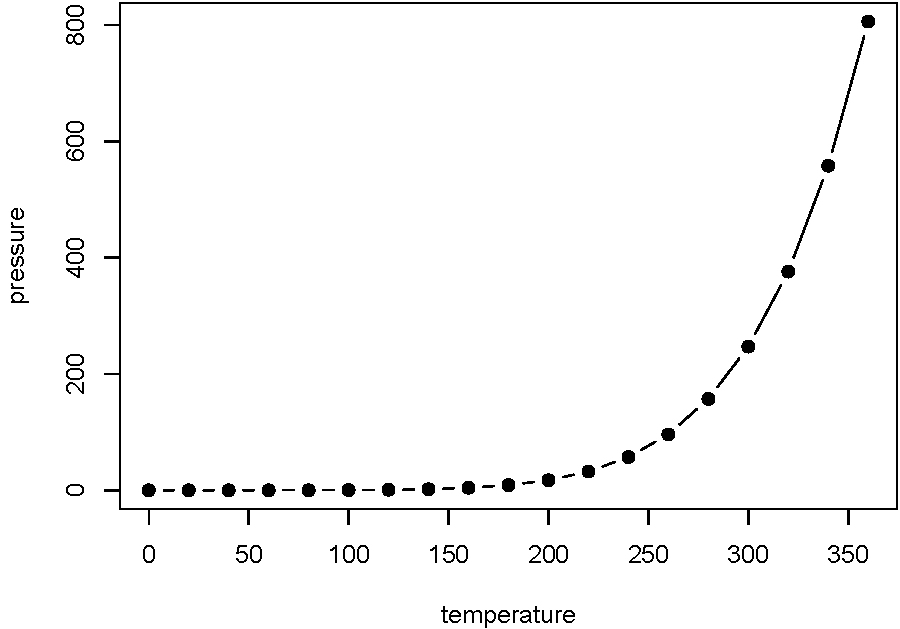
\includegraphics[width=0.7\linewidth]{bookdown-book-zhCN_files/figure-latex/no-caption-1}

The disadvantage of typesetting figures in this way is that when there is not enough space on the current page to place a figure, it may either reach the bottom of the page (hence exceeds the page margin), or be pushed to the next page, leaving a large white margin at the bottom of the current page. That is basically why there are ``floating environments''\index{floating environment} in LaTeX: elements that cannot be split over multiple pages (like figures) are put in floating environments, so they can float to a page that has enough space to hold them. There is also a disadvantage of floating things forward or backward, though. That is, readers may have to jump to a different page to find the figure mentioned on the current page. This is simply a natural consequence of having to typeset things on multiple pages of fixed sizes. This issue does not exist in HTML, however, since everything can be placed continuously on one single page (presumably with infinite height), and there is no need to split anything across multiple pages of the same page size.

If we assign a figure caption to a code chunk via the chunk option \texttt{fig.cap}, R plots will be put into figure environments, which will be automatically labeled and numbered, and can also be cross-referenced. The label of a figure environment is generated from the label of the code chunk, e.g., if the chunk label is \texttt{foo}, the figure label will be \texttt{fig:foo} (the prefix \texttt{fig:} is added before \texttt{foo}). To reference a figure\index{cross-reference}, use the syntax \texttt{\textbackslash{}@ref(label)},\footnote{Do not forget the leading backslash! And also note the parentheses \texttt{()} after \texttt{ref}; they are not curly braces \texttt{\{\}}.} where \texttt{label} is the figure label, e.g., \texttt{fig:foo}.

To take advantage of Markdown formatting \emph{within} the figure caption, you will need to use text references (see Section \ref{text-references}). For example, a figure caption that contains \texttt{\_italic\ text\_} will not work when the output format is LaTeX/PDF, since the underscore is a special character in LaTeX, but if you use text references, \texttt{\_italic\ text\_} will be translated to LaTeX code when the output is LaTeX.

\begin{rmdimportant}
If you want to cross-reference figures or tables generated from a code chunk, please make sure the chunk label only contains \emph{alphanumeric} characters (a-z, A-Z, 0-9), slashes (/), or dashes (-).
\end{rmdimportant}

The chunk option \texttt{fig.asp} can be used to set the aspect ratio of plots, i.e., the ratio of figure height/width. If the figure width is 6 inches (\texttt{fig.width\ =\ 6}) and \texttt{fig.asp\ =\ 0.7}, the figure height will be automatically calculated from \texttt{fig.width\ *\ fig.asp\ =\ 6\ *\ 0.7\ =\ 4.2}. Figure \ref{fig:pressure-plot} is an example using the chunk options \texttt{fig.asp\ =\ 0.7}, \texttt{fig.width\ =\ 6}, and \texttt{fig.align\ =\ \textquotesingle{}center\textquotesingle{}}, generated from the code below:

\begin{Shaded}
\begin{Highlighting}[]
\FunctionTok{par}\NormalTok{(}\AttributeTok{mar =} \FunctionTok{c}\NormalTok{(}\DecValTok{4}\NormalTok{, }\DecValTok{4}\NormalTok{, .}\DecValTok{1}\NormalTok{, .}\DecValTok{1}\NormalTok{))}
\FunctionTok{plot}\NormalTok{(pressure, }\AttributeTok{pch =} \DecValTok{19}\NormalTok{, }\AttributeTok{type =} \StringTok{\textquotesingle{}b\textquotesingle{}}\NormalTok{)}
\end{Highlighting}
\end{Shaded}

\begin{figure}

{\centering 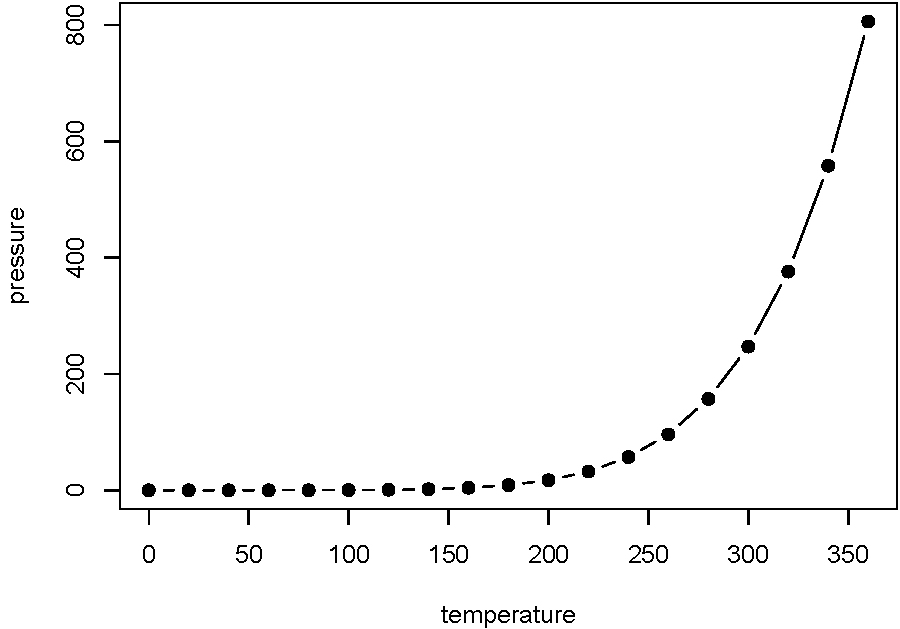
\includegraphics[width=0.9\linewidth]{bookdown-book-zhCN_files/figure-latex/pressure-plot-1} 

}

\caption{A figure example with the specified aspect ratio, width, and alignment.}\label{fig:pressure-plot}
\end{figure}

The actual size of a plot is determined by the chunk options \texttt{fig.width} and \texttt{fig.height} (the size of the plot generated from a graphical device), and we can specify the output size of plots via the chunk options \texttt{out.width} and \texttt{out.height}. The possible value of these two options depends on the output format of the document. For example, \texttt{out.width\ =\ \textquotesingle{}30\%\textquotesingle{}} is a valid value for HTML output, but not for LaTeX/PDF output. However, \textbf{knitr} will automatically convert a percentage value for \texttt{out.width} of the form \texttt{x\%} to \texttt{(x\ /\ 100)\ \textbackslash{}linewidth}, e.g., \texttt{out.width\ =\ \textquotesingle{}70\%\textquotesingle{}} will be treated as \texttt{.7\textbackslash{}linewidth} when the output format is LaTeX. This makes it possible to specify a relative width of a plot in a consistent manner. Figure \ref{fig:cars-plot} is an example of \texttt{out.width\ =\ 70\%}.

\begin{Shaded}
\begin{Highlighting}[]
\FunctionTok{par}\NormalTok{(}\AttributeTok{mar =} \FunctionTok{c}\NormalTok{(}\DecValTok{4}\NormalTok{, }\DecValTok{4}\NormalTok{, .}\DecValTok{1}\NormalTok{, .}\DecValTok{1}\NormalTok{))}
\FunctionTok{plot}\NormalTok{(cars, }\AttributeTok{pch =} \DecValTok{19}\NormalTok{)}
\end{Highlighting}
\end{Shaded}

\begin{figure}
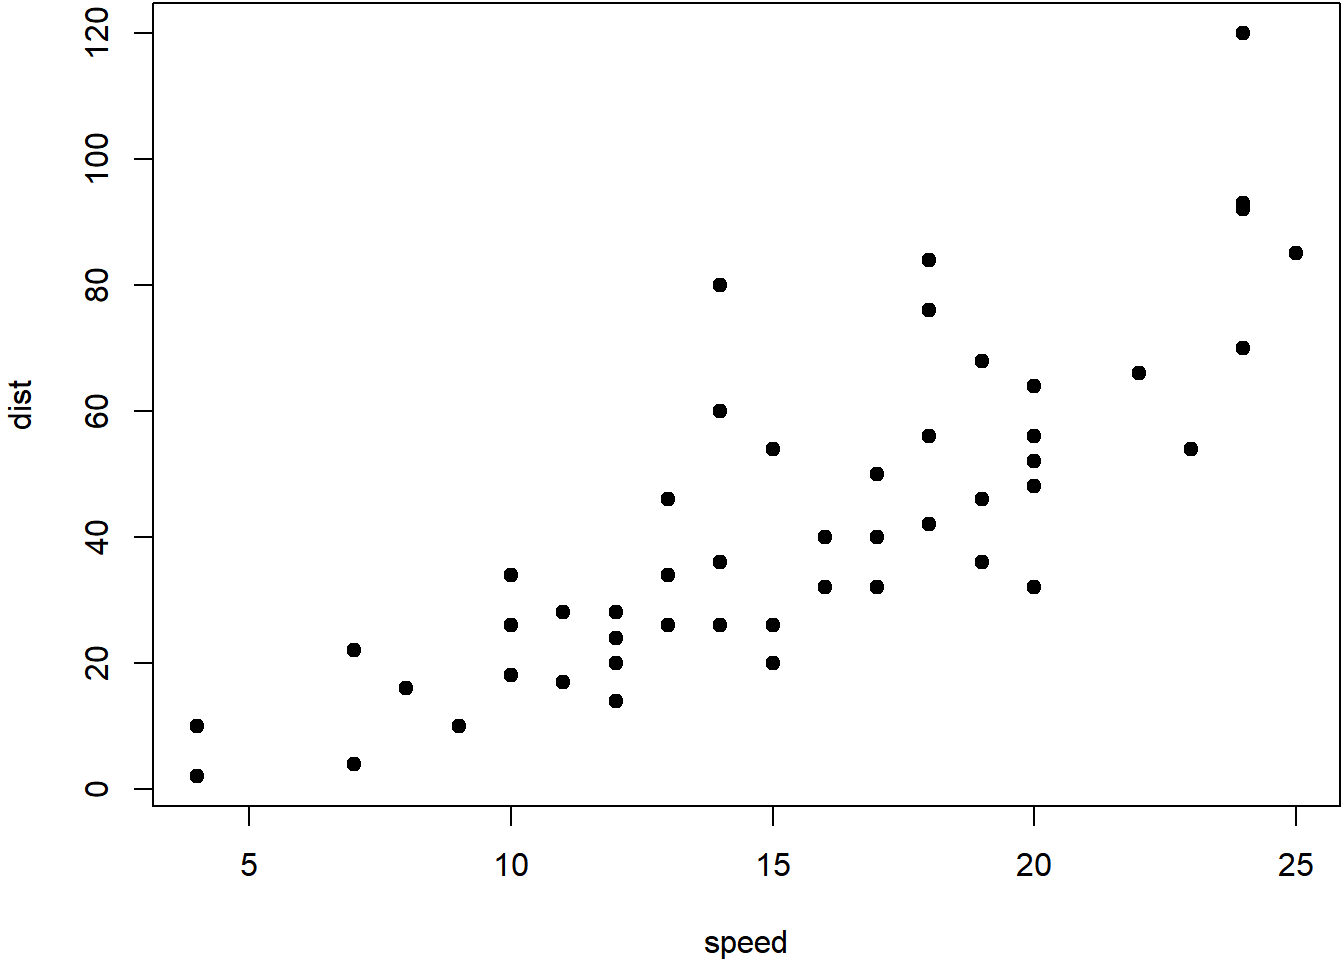
\includegraphics[width=0.7\linewidth]{bookdown-book-zhCN_files/figure-latex/cars-plot-1} \caption{A figure example with a relative width 70\%.}\label{fig:cars-plot}
\end{figure}

If you want to put multiple plots in one figure environment, you must use the chunk option \texttt{fig.show\ =\ \textquotesingle{}hold\textquotesingle{}} to hold multiple plots from a code chunk and include them in one environment. You can also place plots side by side if the sum of the width of all plots is smaller than or equal to the current line width. For example, if two plots have the same width \texttt{50\%}, they will be placed side by side. Similarly, you can specify \texttt{out.width\ =\ \textquotesingle{}33\%\textquotesingle{}} to arrange three plots on one line. Figure \ref{fig:multi-plots} is an example of two plots, each with a width of \texttt{50\%}.

\begin{Shaded}
\begin{Highlighting}[]
\FunctionTok{par}\NormalTok{(}\AttributeTok{mar =} \FunctionTok{c}\NormalTok{(}\DecValTok{4}\NormalTok{, }\DecValTok{4}\NormalTok{, .}\DecValTok{1}\NormalTok{, .}\DecValTok{1}\NormalTok{))}
\FunctionTok{plot}\NormalTok{(pressure, }\AttributeTok{pch =} \DecValTok{19}\NormalTok{, }\AttributeTok{type =} \StringTok{\textquotesingle{}b\textquotesingle{}}\NormalTok{)}
\FunctionTok{plot}\NormalTok{(cars, }\AttributeTok{pch =} \DecValTok{19}\NormalTok{)}
\end{Highlighting}
\end{Shaded}

\begin{figure}
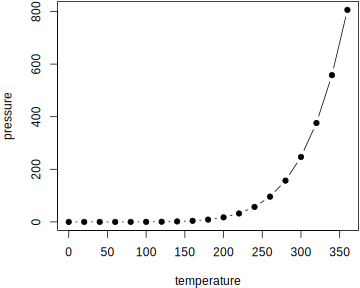
\includegraphics[width=0.5\linewidth]{bookdown-book-zhCN_files/figure-latex/multi-plots-1} 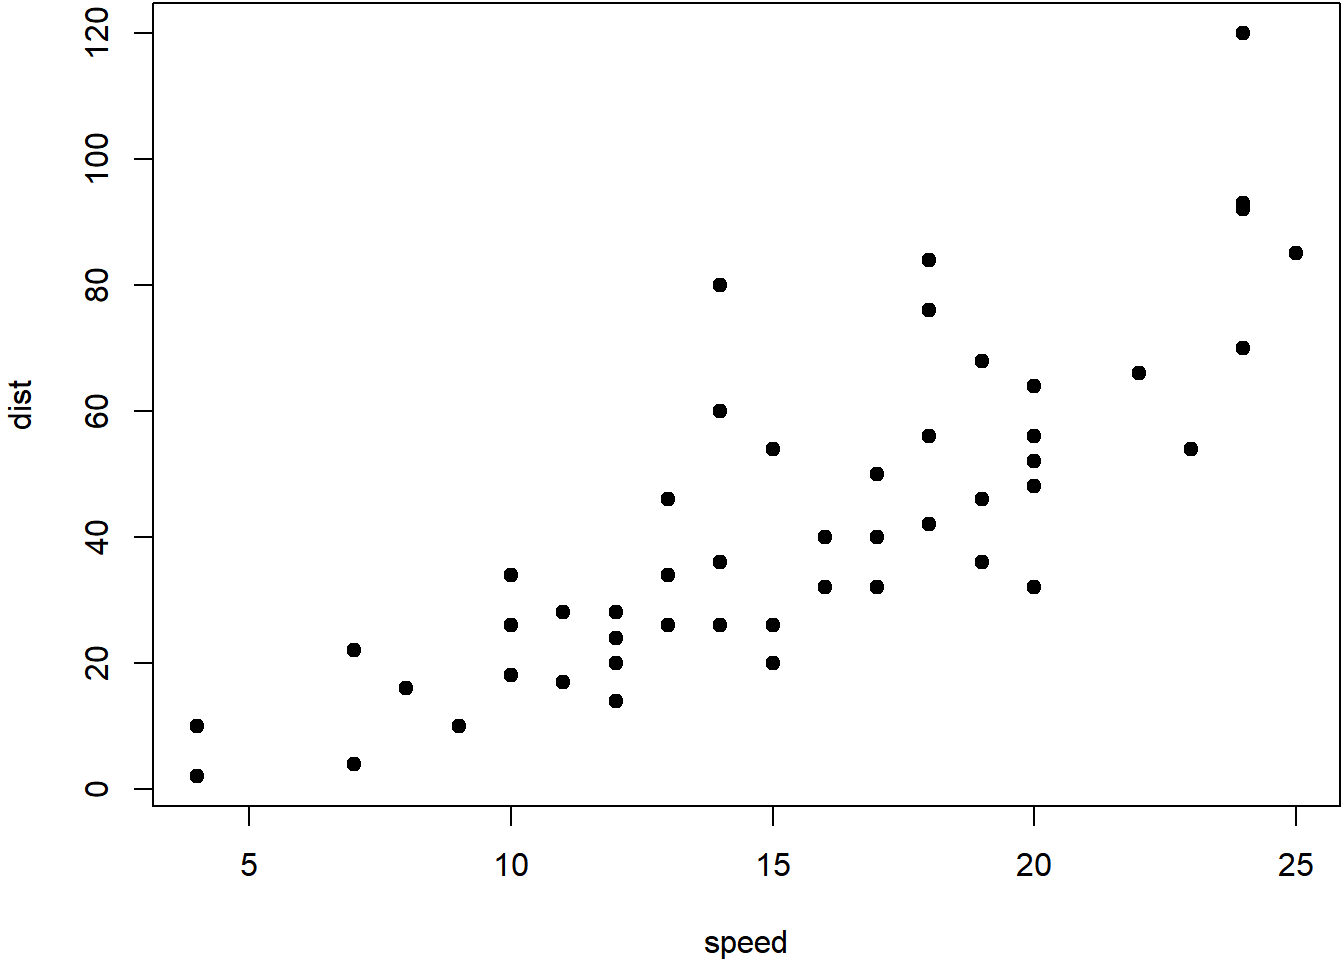
\includegraphics[width=0.5\linewidth]{bookdown-book-zhCN_files/figure-latex/multi-plots-2} \caption{Two plots placed side by side.}\label{fig:multi-plots}
\end{figure}

Sometimes you may have certain images that are not generated from R code, and you can include them in R Markdown via the function \texttt{knitr::include\_graphics()}. Figure \ref{fig:knitr-logo} is an example of three \textbf{knitr} logos included in a figure environment. You may pass one or multiple image paths to the \texttt{include\_graphics()}\index{knitr::include\_graphics()} function, and all chunk options that apply to normal R plots also apply to these images, e.g., you can use \texttt{out.width\ =\ \textquotesingle{}33\%\textquotesingle{}} to set the widths of these images in the output document.

\begin{Shaded}
\begin{Highlighting}[]
\NormalTok{knitr}\SpecialCharTok{::}\FunctionTok{include\_graphics}\NormalTok{(}\FunctionTok{rep}\NormalTok{(}\StringTok{\textquotesingle{}images/knit{-}logo.png\textquotesingle{}}\NormalTok{, }\DecValTok{3}\NormalTok{))}
\end{Highlighting}
\end{Shaded}

\begin{figure}
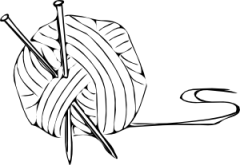
\includegraphics[width=0.328\linewidth]{images/knit-logo} 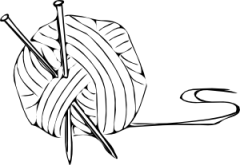
\includegraphics[width=0.328\linewidth]{images/knit-logo} 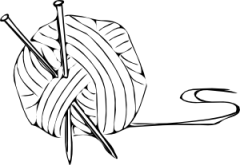
\includegraphics[width=0.328\linewidth]{images/knit-logo} \caption{Three knitr logos included in the document from an external PNG image file.}\label{fig:knitr-logo}
\end{figure}

There are a few advantages of using \texttt{include\_graphics()}:

\begin{enumerate}
\def\labelenumi{\arabic{enumi}.}
\tightlist
\item
  You do not need to worry about the document output format, e.g., when the output format is LaTeX, you may have to use the LaTeX command \texttt{\textbackslash{}includegraphics\{\}} to include an image, and when the output format is Markdown, you have to use \texttt{!{[}{]}()}. The function \texttt{include\_graphics()} in \textbf{knitr} takes care of these details automatically.
\item
  The syntax for controlling the image attributes is the same as when images are generated from R code, e.g., chunk options \texttt{fig.cap}, \texttt{out.width}, and \texttt{fig.show} still have the same meanings.
\item
  \texttt{include\_graphics()} can be smart enough to use PDF graphics automatically when the output format is LaTeX and the PDF graphics files exist, e.g., an image path \texttt{foo/bar.png} can be automatically replaced with \texttt{foo/bar.pdf} if the latter exists. PDF images often have better qualities than raster images in LaTeX/PDF output. To make use of this feature, set the argument \texttt{auto\_pdf\ =\ TRUE}, or set the global option \texttt{options(knitr.graphics.auto\_pdf\ =\ TRUE)} to enable this feature globally in an R session.
\item
  You can easily scale these images proportionally using the same ratio. This can be done via the \texttt{dpi} argument (dots per inch), which takes the value from the chunk option \texttt{dpi} by default. If it is a numeric value and the chunk option \texttt{out.width} is not set, the output width of an image will be its actual width (in pixels) divided by \texttt{dpi}, and the unit will be inches. For example, for an image with the size 672 x 480, its output width will be 7 inches (\texttt{7in}) when \texttt{dpi\ =\ 96}. This feature requires the package \textbf{png} and/or \textbf{jpeg} to be installed. You can always override the automatic calculation of width in inches by providing a non-NULL value to the chunk option \texttt{out.width}, or use \texttt{include\_graphics(dpi\ =\ NA)}.
\end{enumerate}

\hypertarget{tables}{%
\section{Tables}\label{tables}}

For now, the most convenient way to generate a table\index{table} is the function \texttt{knitr::kable()}, because there are some internal tricks in \textbf{knitr} to make it work with \textbf{bookdown} and users do not have to know anything about these implementation details. We will explain how to use other packages and functions later in this section.

Like figures, tables with captions will also be numbered and can be referenced\index{cross-reference}. The \texttt{kable()} function will automatically generate a label for a table environment, which is the prefix \texttt{tab:} plus the chunk label. For example, the table label for a code chunk with the label \texttt{foo} will be \texttt{tab:foo}, and we can still use the syntax \texttt{\textbackslash{}@ref(label)} to reference the table. Table \ref{tab:table-single} is a simple example.

\begin{Shaded}
\begin{Highlighting}[]
\NormalTok{knitr}\SpecialCharTok{::}\FunctionTok{kable}\NormalTok{(}
  \FunctionTok{head}\NormalTok{(mtcars[, }\DecValTok{1}\SpecialCharTok{:}\DecValTok{8}\NormalTok{], }\DecValTok{10}\NormalTok{), }\AttributeTok{booktabs =} \ConstantTok{TRUE}\NormalTok{,}
  \AttributeTok{caption =} \StringTok{\textquotesingle{}A table of the first 10 rows of the mtcars data.\textquotesingle{}}
\NormalTok{)}
\end{Highlighting}
\end{Shaded}

\begin{table}

\caption{\label{tab:table-single}A table of the first 10 rows of the mtcars data.}
\centering
\begin{tabular}[t]{lrrrrrrrr}
\toprule
  & mpg & cyl & disp & hp & drat & wt & qsec & vs\\
\midrule
Mazda RX4 & 21.0 & 6 & 160.0 & 110 & 3.90 & 2.620 & 16.46 & 0\\
Mazda RX4 Wag & 21.0 & 6 & 160.0 & 110 & 3.90 & 2.875 & 17.02 & 0\\
Datsun 710 & 22.8 & 4 & 108.0 & 93 & 3.85 & 2.320 & 18.61 & 1\\
Hornet 4 Drive & 21.4 & 6 & 258.0 & 110 & 3.08 & 3.215 & 19.44 & 1\\
Hornet Sportabout & 18.7 & 8 & 360.0 & 175 & 3.15 & 3.440 & 17.02 & 0\\
\addlinespace
Valiant & 18.1 & 6 & 225.0 & 105 & 2.76 & 3.460 & 20.22 & 1\\
Duster 360 & 14.3 & 8 & 360.0 & 245 & 3.21 & 3.570 & 15.84 & 0\\
Merc 240D & 24.4 & 4 & 146.7 & 62 & 3.69 & 3.190 & 20.00 & 1\\
Merc 230 & 22.8 & 4 & 140.8 & 95 & 3.92 & 3.150 & 22.90 & 1\\
Merc 280 & 19.2 & 6 & 167.6 & 123 & 3.92 & 3.440 & 18.30 & 1\\
\bottomrule
\end{tabular}
\end{table}

If you want to put multiple tables in a single table environment, wrap the data objects (usually data frames in R) into a list. See Table \ref{tab:table-multi} for an example. Please note that this feature is only available in HTML and PDF output.

\begin{Shaded}
\begin{Highlighting}[]
\NormalTok{knitr}\SpecialCharTok{::}\FunctionTok{kable}\NormalTok{(}
  \FunctionTok{list}\NormalTok{(}
    \FunctionTok{head}\NormalTok{(iris[, }\DecValTok{1}\SpecialCharTok{:}\DecValTok{2}\NormalTok{], }\DecValTok{3}\NormalTok{),}
    \FunctionTok{head}\NormalTok{(mtcars[, }\DecValTok{1}\SpecialCharTok{:}\DecValTok{3}\NormalTok{], }\DecValTok{5}\NormalTok{)}
\NormalTok{  ),}
  \AttributeTok{caption =} \StringTok{\textquotesingle{}A Tale of Two Tables.\textquotesingle{}}\NormalTok{, }\AttributeTok{booktabs =} \ConstantTok{TRUE}
\NormalTok{)}
\end{Highlighting}
\end{Shaded}

\begin{table}
\caption{\label{tab:table-multi}A Tale of Two Tables.}

\centering
\begin{tabular}[t]{rr}
\toprule
Sepal.Length & Sepal.Width\\
\midrule
5.1 & 3.5\\
4.9 & 3.0\\
4.7 & 3.2\\
\bottomrule
\end{tabular}
\centering
\begin{tabular}[t]{lrrr}
\toprule
  & mpg & cyl & disp\\
\midrule
Mazda RX4 & 21.0 & 6 & 160\\
Mazda RX4 Wag & 21.0 & 6 & 160\\
Datsun 710 & 22.8 & 4 & 108\\
Hornet 4 Drive & 21.4 & 6 & 258\\
Hornet Sportabout & 18.7 & 8 & 360\\
\bottomrule
\end{tabular}
\end{table}

When you do not want a table to float in PDF, you may use the LaTeX package \href{https://www.ctan.org/pkg/longtable}{\textbf{longtable},}\index{longtable} which can break a table across multiple pages. To use \textbf{longtable}, pass \texttt{longtable\ =\ TRUE} to \texttt{kable()}, and make sure to include \texttt{\textbackslash{}usepackage\{longtable\}} in the LaTeX preamble (see Section \ref{yaml-options} for how to customize the LaTeX preamble). Of course, this is irrelevant to HTML output, since tables in HTML do not need to float.

\begin{Shaded}
\begin{Highlighting}[]
\NormalTok{knitr}\SpecialCharTok{::}\FunctionTok{kable}\NormalTok{(}
\NormalTok{  iris[}\DecValTok{1}\SpecialCharTok{:}\DecValTok{55}\NormalTok{, ], }\AttributeTok{longtable =} \ConstantTok{TRUE}\NormalTok{, }\AttributeTok{booktabs =} \ConstantTok{TRUE}\NormalTok{,}
  \AttributeTok{caption =} \StringTok{\textquotesingle{}A table generated by the longtable package.\textquotesingle{}}
\NormalTok{)}
\end{Highlighting}
\end{Shaded}

\begin{longtable}[t]{rrrrl}
\caption{\label{tab:longtable}A table generated by the longtable package.}\\
\toprule
Sepal.Length & Sepal.Width & Petal.Length & Petal.Width & Species\\
\midrule
5.1 & 3.5 & 1.4 & 0.2 & setosa\\
4.9 & 3.0 & 1.4 & 0.2 & setosa\\
4.7 & 3.2 & 1.3 & 0.2 & setosa\\
4.6 & 3.1 & 1.5 & 0.2 & setosa\\
5.0 & 3.6 & 1.4 & 0.2 & setosa\\
\addlinespace
5.4 & 3.9 & 1.7 & 0.4 & setosa\\
4.6 & 3.4 & 1.4 & 0.3 & setosa\\
5.0 & 3.4 & 1.5 & 0.2 & setosa\\
4.4 & 2.9 & 1.4 & 0.2 & setosa\\
4.9 & 3.1 & 1.5 & 0.1 & setosa\\
\addlinespace
5.4 & 3.7 & 1.5 & 0.2 & setosa\\
4.8 & 3.4 & 1.6 & 0.2 & setosa\\
4.8 & 3.0 & 1.4 & 0.1 & setosa\\
4.3 & 3.0 & 1.1 & 0.1 & setosa\\
5.8 & 4.0 & 1.2 & 0.2 & setosa\\
\addlinespace
5.7 & 4.4 & 1.5 & 0.4 & setosa\\
5.4 & 3.9 & 1.3 & 0.4 & setosa\\
5.1 & 3.5 & 1.4 & 0.3 & setosa\\
5.7 & 3.8 & 1.7 & 0.3 & setosa\\
5.1 & 3.8 & 1.5 & 0.3 & setosa\\
\addlinespace
5.4 & 3.4 & 1.7 & 0.2 & setosa\\
5.1 & 3.7 & 1.5 & 0.4 & setosa\\
4.6 & 3.6 & 1.0 & 0.2 & setosa\\
5.1 & 3.3 & 1.7 & 0.5 & setosa\\
4.8 & 3.4 & 1.9 & 0.2 & setosa\\
\addlinespace
5.0 & 3.0 & 1.6 & 0.2 & setosa\\
5.0 & 3.4 & 1.6 & 0.4 & setosa\\
5.2 & 3.5 & 1.5 & 0.2 & setosa\\
5.2 & 3.4 & 1.4 & 0.2 & setosa\\
4.7 & 3.2 & 1.6 & 0.2 & setosa\\
\addlinespace
4.8 & 3.1 & 1.6 & 0.2 & setosa\\
5.4 & 3.4 & 1.5 & 0.4 & setosa\\
5.2 & 4.1 & 1.5 & 0.1 & setosa\\
5.5 & 4.2 & 1.4 & 0.2 & setosa\\
4.9 & 3.1 & 1.5 & 0.2 & setosa\\
\addlinespace
5.0 & 3.2 & 1.2 & 0.2 & setosa\\
5.5 & 3.5 & 1.3 & 0.2 & setosa\\
4.9 & 3.6 & 1.4 & 0.1 & setosa\\
4.4 & 3.0 & 1.3 & 0.2 & setosa\\
5.1 & 3.4 & 1.5 & 0.2 & setosa\\
\addlinespace
5.0 & 3.5 & 1.3 & 0.3 & setosa\\
4.5 & 2.3 & 1.3 & 0.3 & setosa\\
4.4 & 3.2 & 1.3 & 0.2 & setosa\\
5.0 & 3.5 & 1.6 & 0.6 & setosa\\
5.1 & 3.8 & 1.9 & 0.4 & setosa\\
\addlinespace
4.8 & 3.0 & 1.4 & 0.3 & setosa\\
5.1 & 3.8 & 1.6 & 0.2 & setosa\\
4.6 & 3.2 & 1.4 & 0.2 & setosa\\
5.3 & 3.7 & 1.5 & 0.2 & setosa\\
5.0 & 3.3 & 1.4 & 0.2 & setosa\\
\addlinespace
7.0 & 3.2 & 4.7 & 1.4 & versicolor\\
6.4 & 3.2 & 4.5 & 1.5 & versicolor\\
6.9 & 3.1 & 4.9 & 1.5 & versicolor\\
5.5 & 2.3 & 4.0 & 1.3 & versicolor\\
6.5 & 2.8 & 4.6 & 1.5 & versicolor\\
\bottomrule
\end{longtable}

Pandoc supports several types of \href{http://pandoc.org/MANUAL.html\#tables}{Markdown tables,} such as simple tables, multiline tables, grid tables, and pipe tables. What \texttt{knitr::kable()} generates is a simple table like this:

\begin{Shaded}
\begin{Highlighting}[]
\AnnotationTok{Table:}\CommentTok{ A simple table in Markdown.}

\NormalTok{ Sepal.Length   Sepal.Width   Petal.Length   Petal.Width}
\NormalTok{{-}{-}{-}{-}{-}{-}{-}{-}{-}{-}{-}{-}{-}  {-}{-}{-}{-}{-}{-}{-}{-}{-}{-}{-}{-}  {-}{-}{-}{-}{-}{-}{-}{-}{-}{-}{-}{-}{-}  {-}{-}{-}{-}{-}{-}{-}{-}{-}{-}{-}{-}}
\InformationTok{          5.1           3.5            1.4           0.2}
\InformationTok{          4.9           3.0            1.4           0.2}
\InformationTok{          4.7           3.2            1.3           0.2}
\InformationTok{          4.6           3.1            1.5           0.2}
\InformationTok{          5.0           3.6            1.4           0.2}
\InformationTok{          5.4           3.9            1.7           0.4}
\end{Highlighting}
\end{Shaded}

You can use any types of Markdown tables in your document. To be able to cross-reference a Markdown table, it must have a labeled caption of the form \texttt{Table:\ (\textbackslash{}\#label)\ Caption\ here}, where \texttt{label} must have the prefix \texttt{tab:}, e.g., \texttt{tab:simple-table}.

If you decide to use other R packages to generate tables, you have to make sure the label for the table environment appears in the beginning of the table caption in the form \texttt{(\textbackslash{}\#label)} (again, \texttt{label} must have the prefix \texttt{tab:}). You have to be very careful about the \emph{portability} of the table generating function: it should work for both HTML and LaTeX output automatically, so it must consider the output format internally (check \texttt{knitr::opts\_knit\$get(\textquotesingle{}rmarkdown.pandoc.to\textquotesingle{})}). When writing out an HTML table, the caption must be written in the \texttt{\textless{}caption\textgreater{}\textless{}/caption\textgreater{}} tag. For simple tables, \texttt{kable()} should suffice. If you have to create complicated tables (e.g., with certain cells spanning across multiple columns/rows), you will have to take the aforementioned issues into consideration.

\hypertarget{cross-references}{%
\section{Cross-references}\label{cross-references}}

We have explained how cross-references\index{cross-reference} work for equations (Section \ref{equations}), theorems (Section \ref{theorems}), figures (Section \ref{figures}), and tables (Section \ref{tables}). In fact, you can also reference sections using the same syntax \texttt{\textbackslash{}@ref(label)}, where \texttt{label} is the section ID. By default, Pandoc will generate an ID for all section headers, e.g., a section \texttt{\#\ Hello\ World} will have an ID \texttt{hello-world}. We recommend you to manually assign an ID to a section header to make sure you do not forget to update the reference label after you change the section header. To assign an ID to a section header, simply add \texttt{\{\#id\}} to the end of the section header. Further attributes of section headers can be set using standard \href{http://pandoc.org/MANUAL.html\#heading-identifiers}{Pandoc syntax}.

When a referenced label cannot be found, you will see two question marks like \ref{fig:does-not-exist}, as well as a warning message in the R console when rendering the book.

You can also create text-based links using explicit or automatic section IDs or even the actual section header text.

\begin{itemize}
\tightlist
\item
  If you are happy with the section header as the link text, use it inside a single set of square brackets:

  \begin{itemize}
  \tightlist
  \item
    \texttt{{[}Section\ header\ text{]}}: example ``\protect\hyperlink{a-single-document}{A single document}'' via \texttt{{[}A\ single\ document{]}}
  \end{itemize}
\item
  There are two ways to specify custom link text:

  \begin{itemize}
  \tightlist
  \item
    \texttt{{[}link\ text{]}{[}Section\ header\ text{]}}, e.g., ``\protect\hyperlink{internationalization}{non-English books}'' via \texttt{{[}non-English\ books{]}{[}Internationalization{]}}
  \item
    \texttt{{[}link\ text{]}(\#ID)}, e.g., ``\protect\hyperlink{tables}{Table stuff}'' via \texttt{{[}Table\ stuff{]}(\#tables)}
  \end{itemize}
\end{itemize}

The Pandoc documentation provides more details on \href{http://pandoc.org/MANUAL.html\#extension-auto_identifiers}{automatic section IDs} and \href{http://pandoc.org/MANUAL.html\#extension-implicit_header_references}{implicit header references.}

Cross-references still work even when we refer to an item that is not on the current page of the PDF or HTML output. For example, see Equation \eqref{eq:binom} and Figure \ref{fig:knitr-logo}.

\hypertarget{custom-blocks}{%
\section{Custom blocks}\label{custom-blocks}}

\begin{rmdimportant}
We recommend that you use the new syntax to create custom blocks, which is introduced in \href{https://bookdown.org/yihui/rmarkdown-cookbook/custom-blocks.html}{Section 9.6 in the \emph{R Markdown Cookbook}} \citep{rmarkdown2020}. We do not recommend using the \texttt{block} or \texttt{block2} engine described below. Those will be deprecated in a future version of \textbf{bookdown}. Please remember to switch to the new syntax for your content if you are still using one of these engines. Thanks for your understanding!

\end{rmdimportant}

You can generate custom blocks\index{custom block} using the \texttt{block} engine in \textbf{knitr}, i.e., the chunk option \texttt{engine\ =\ \textquotesingle{}block\textquotesingle{}}, or the more compact syntax \texttt{\textasciigrave{}\textasciigrave{}\textasciigrave{}\{block\}}. This engine should be used in conjunction with the chunk option \texttt{type}, which takes a character string. When the \texttt{block} engine is used, it generates a \texttt{\textless{}div\textgreater{}} to wrap the chunk content if the output format is HTML, and a LaTeX environment if the output is LaTeX. The \texttt{type} option specifies the class of the \texttt{\textless{}div\textgreater{}} and the name of the LaTeX environment. For example, the HTML output of this chunk

\begin{Shaded}
\begin{Highlighting}[]
\InformationTok{\textasciigrave{}\textasciigrave{}\textasciigrave{}\{block, type=\textquotesingle{}FOO\textquotesingle{}\}}
\InformationTok{Some text for this block.}
\InformationTok{\textasciigrave{}\textasciigrave{}\textasciigrave{}}
\end{Highlighting}
\end{Shaded}

will be this:

\begin{Shaded}
\begin{Highlighting}[]
\KeywordTok{\textless{}div}\OtherTok{ class=}\StringTok{"FOO"}\KeywordTok{\textgreater{}}
\NormalTok{Some text for this block.}
\KeywordTok{\textless{}/div\textgreater{}}
\end{Highlighting}
\end{Shaded}

and the LaTeX output will be this:

\begin{Shaded}
\begin{Highlighting}[]
\KeywordTok{\textbackslash{}begin}\NormalTok{\{}\ExtensionTok{FOO}\NormalTok{\}}
\NormalTok{Some text for this block.}
\KeywordTok{\textbackslash{}end}\NormalTok{\{}\ExtensionTok{FOO}\NormalTok{\}}
\end{Highlighting}
\end{Shaded}

It is up to the book author how to define the style of the block. You can define the style of the \texttt{\textless{}div\textgreater{}} in CSS and include it in the output via the \texttt{includes} option in the YAML metadata. Similarly, you may define the LaTeX environment via \texttt{\textbackslash{}newenvironment} and include the definition in the LaTeX output via the \texttt{includes} option. For example, we may save the following style in a CSS file, say, \texttt{style.css}:

\begin{Shaded}
\begin{Highlighting}[]
\NormalTok{div}\FunctionTok{.FOO}\NormalTok{ \{}
  \KeywordTok{font{-}weight}\NormalTok{: }\DecValTok{bold}\OperatorTok{;}
  \KeywordTok{color}\NormalTok{: }\ConstantTok{red}\OperatorTok{;}
\NormalTok{\}}
\end{Highlighting}
\end{Shaded}

And the YAML metadata of the R Markdown document can be:

\begin{Shaded}
\begin{Highlighting}[]
\PreprocessorTok{{-}{-}{-}}
\FunctionTok{output}\KeywordTok{:}
\AttributeTok{  bookdown:}\FunctionTok{:html\_book}\KeywordTok{:}
\AttributeTok{    }\FunctionTok{includes}\KeywordTok{:}
\AttributeTok{      }\FunctionTok{in\_header}\KeywordTok{:}\AttributeTok{ style.css}
\PreprocessorTok{{-}{-}{-}}
\end{Highlighting}
\end{Shaded}

We have defined a few types of blocks for this book to show notes, tips, and warnings, etc. Below are some examples:

\begin{rmdnote}
R is free software and comes with ABSOLUTELY NO WARRANTY.
You are welcome to redistribute it under the terms of the
GNU General Public License versions 2 or 3.
For more information about these matters see
\url{http://www.gnu.org/licenses/}.
\end{rmdnote}

\begin{rmdcaution}
R is free software and comes with ABSOLUTELY NO WARRANTY.
You are welcome to redistribute it under the terms of the
GNU General Public License versions 2 or 3.
For more information about these matters see
\url{http://www.gnu.org/licenses/}.
\end{rmdcaution}

\begin{rmdimportant}
R is free software and comes with ABSOLUTELY NO WARRANTY.
You are welcome to redistribute it under the terms of the
GNU General Public License versions 2 or 3.
For more information about these matters see
\url{http://www.gnu.org/licenses/}.
\end{rmdimportant}

\begin{rmdtip}
R is free software and comes with ABSOLUTELY NO WARRANTY.
You are welcome to redistribute it under the terms of the
GNU General Public License versions 2 or 3.
For more information about these matters see
\url{http://www.gnu.org/licenses/}.
\end{rmdtip}

\begin{rmdwarning}
R is free software and comes with ABSOLUTELY NO WARRANTY.
You are welcome to redistribute it under the terms of the
GNU General Public License versions 2 or 3.
For more information about these matters see
\url{http://www.gnu.org/licenses/}.
\end{rmdwarning}

The \textbf{knitr} \texttt{block} engine was designed to display simple content (typically a paragraph of plain text). You can use simple formatting syntax such as making certain words bold or italic, but more advanced syntax such as citations and cross-references will not work. However, there is an alternative engine named \texttt{block2} that supports arbitrary Markdown syntax, e.g.,

\begin{Shaded}
\begin{Highlighting}[]
\InformationTok{\textasciigrave{}\textasciigrave{}\textasciigrave{}\{block2, type=\textquotesingle{}FOO\textquotesingle{}\}}
\InformationTok{Some text for this block [@citation{-}key].}

\InformationTok{{-} a list item}
\InformationTok{{-} another item}

\InformationTok{More text.}
\InformationTok{\textasciigrave{}\textasciigrave{}\textasciigrave{}}
\end{Highlighting}
\end{Shaded}

The \texttt{block2} engine should also be faster than the \texttt{block} engine if you have a lot of custom blocks in the document, but its implementation was based on \href{https://github.com/jgm/pandoc/issues/2453}{a hack,} so we are not 100\% sure if it is always going to work in the future. We have not seen problems with Pandoc v1.17.2 yet.

One more caveat for the \texttt{block2} engine: if the last element in the block is not an ordinary paragraph, you must leave a blank line at the end, e.g.,

\begin{Shaded}
\begin{Highlighting}[]
\InformationTok{\textasciigrave{}\textasciigrave{}\textasciigrave{}\{block2, type=\textquotesingle{}FOO\textquotesingle{}\}}
\InformationTok{Some text for this block [@citation{-}key].}

\InformationTok{{-} a list item}
\InformationTok{{-} another item}
\InformationTok{{-} end the list with a blank line}

\InformationTok{\textasciigrave{}\textasciigrave{}\textasciigrave{}}
\end{Highlighting}
\end{Shaded}

The theorem and proof environments in Section \ref{theorems} are actually implemented through the \texttt{block2} engine.

For all custom blocks based on the \texttt{block} or \texttt{block2} engine, there is one chunk option \texttt{echo} that you can use to show (\texttt{echo\ =\ TRUE}) or hide (\texttt{echo\ =\ FALSE}) the blocks.

\hypertarget{citations}{%
\section{Citations}\label{citations}}

Pandoc offers two methods for managing citations\index{citation} and bibliographic references in a document.

\begin{enumerate}
\def\labelenumi{\arabic{enumi}.}
\item
  The default method is to use a Pandoc helper program called \href{https://github.com/jgm/pandoc-citeproc}{\texttt{pandoc-citeproc}}, which follows the specifications of the \href{http://docs.citationstyles.org/en/1.0.1/specification.html}{Citation Style Language (CSL)} and obtains specific formatting instructions from one of the huge number of available \href{https://www.zotero.org/styles/}{CSL style files.}
\item
  Users may also choose to use either \href{https://ctan.org/pkg/natbib}{\textbf{natbib}} (based on \texttt{bibtex}) or \href{https://ctan.org/pkg/biblatex}{\textbf{biblatex}} as a ``citation package''. In this case, the bibliographic data files need to be in the \texttt{bibtex} or \texttt{biblatex} format, and the document output format is limited to PDF. Again, various bibliographic styles are available (please consult the documentation of these packages).

  To use \textbf{natbib} or \textbf{biblatex} to process references, you can set the \texttt{citation\_package} option of the R Markdown output format, e.g.,

\begin{Shaded}
\begin{Highlighting}[]
\FunctionTok{output}\KeywordTok{:}
\AttributeTok{  }\FunctionTok{pdf\_document}\KeywordTok{:}
\AttributeTok{    }\FunctionTok{citation\_package}\KeywordTok{:}\AttributeTok{ natbib}
\AttributeTok{  bookdown:}\FunctionTok{:pdf\_book}\KeywordTok{:}
\AttributeTok{    }\FunctionTok{citation\_package}\KeywordTok{:}\AttributeTok{ biblatex}
\end{Highlighting}
\end{Shaded}
\end{enumerate}

Even if you choose \texttt{natbib} or \texttt{biblatex} for PDF output, all other output formats will be using \texttt{pandoc-citeproc}. If you use matching styles (e.g., \texttt{biblio-style:\ apa} for \texttt{biblatex} along with \texttt{csl:\ apa.csl} for \texttt{pandoc-citeproc}), output to PDF and to non-PDF formats will be very similar, though not necessarily identical.

For any non-PDF output format, \texttt{pandoc-citeproc} is the only available option. If consistency across PDF and non-PDF output
formats is important, use \texttt{pandoc-citeproc} throughout.

The bibliographic data can be in several formats. We have only shown examples of BibTeX databases in this section, and please see the \href{https://pandoc.org/MANUAL.html\#citations}{``Citations''} section of the Pandoc manual for other possible formats.

A BibTeX database is a plain-text file (with the conventional filename extension \texttt{.bib}) that consists of bibliography entries like this:

\begin{Shaded}
\begin{Highlighting}[]
\VariableTok{@Manual}\NormalTok{\{}\OtherTok{R}\NormalTok{{-}}\OtherTok{base}\NormalTok{,}
  \DataTypeTok{title}\NormalTok{ = \{R: A Language and Environment for Statistical}
\NormalTok{    Computing\},}
  \DataTypeTok{author}\NormalTok{ = \{\{R Core Team\}\},}
  \DataTypeTok{organization}\NormalTok{ = \{R Foundation for Statistical Computing\},}
  \DataTypeTok{address}\NormalTok{ = \{Vienna, Austria\},}
  \DataTypeTok{year}\NormalTok{ = \{2016\},}
  \DataTypeTok{url}\NormalTok{ = \{https://www.R{-}project.org/\},}
\NormalTok{\}}
\end{Highlighting}
\end{Shaded}

A bibliography entry starts with \texttt{@type\{}, where \texttt{type} may be \texttt{article}, \texttt{book}, \texttt{manual}, and so on.\footnote{The type name is case-insensitive, so it does not matter if it is \texttt{manual}, \texttt{Manual}, or \texttt{MANUAL}.} Then there is a citation key, like \texttt{R-base} in the above example. To cite an entry, use \texttt{@key} or \texttt{{[}@key{]}} (the latter puts the citation in braces), e.g., \texttt{@R-base} is rendered as \citet{R-base}, and \texttt{{[}@R-base{]}} generates ``\citep{R-base}''. If you are familiar with the \textbf{natbib} package in LaTeX, \texttt{@key} is basically \texttt{\textbackslash{}citet\{key\}}, and \texttt{{[}@key{]}} is equivalent to \texttt{\textbackslash{}citep\{key\}}.

There are a number of fields in a bibliography entry, such as \texttt{title}, \texttt{author}, and \texttt{year}, etc. You may see \url{https://en.wikipedia.org/wiki/BibTeX} for possible types of entries and fields in BibTeX.

There is a helper function \texttt{write\_bib()} in \textbf{knitr} to generate BibTeX entries automatically for R packages, e.g.,

\begin{Shaded}
\begin{Highlighting}[]
\CommentTok{\# the second argument can be a .bib file}
\NormalTok{knitr}\SpecialCharTok{::}\FunctionTok{write\_bib}\NormalTok{(}\FunctionTok{c}\NormalTok{(}\StringTok{\textquotesingle{}knitr\textquotesingle{}}\NormalTok{, }\StringTok{\textquotesingle{}stringr\textquotesingle{}}\NormalTok{), }\StringTok{\textquotesingle{}\textquotesingle{}}\NormalTok{, }\AttributeTok{width =} \DecValTok{60}\NormalTok{)}
\end{Highlighting}
\end{Shaded}

\begin{verbatim}
@Manual{R-knitr,
  title = {knitr: A General-Purpose Package for Dynamic
    Report Generation in R},
  author = {Yihui Xie},
  year = {2021},
  note = {R package version 1.33},
  url = {https://yihui.org/knitr/},
}

@Manual{R-stringr,
  title = {stringr: Simple, Consistent Wrappers for Common
    String Operations},
  author = {Hadley Wickham},
  year = {2019},
  note = {R package version 1.4.0},
  url = {https://CRAN.R-project.org/package=stringr},
}

@Book{knitr2015,
  title = {Dynamic Documents with {R} and knitr},
  author = {Yihui Xie},
  publisher = {Chapman and Hall/CRC},
  address = {Boca Raton, Florida},
  year = {2015},
  edition = {2nd},
  note = {ISBN 978-1498716963},
  url = {https://yihui.org/knitr/},
}

@InCollection{knitr2014,
  booktitle = {Implementing Reproducible Computational
    Research},
  editor = {Victoria Stodden and Friedrich Leisch and Roger
    D. Peng},
  title = {knitr: A Comprehensive Tool for Reproducible
    Research in {R}},
  author = {Yihui Xie},
  publisher = {Chapman and Hall/CRC},
  year = {2014},
  note = {ISBN 978-1466561595},
  url = {http://www.crcpress.com/product/isbn/
    9781466561595},
}
\end{verbatim}

Once you have one or multiple \texttt{.bib} files, you may use the field \texttt{bibliography} in the YAML metadata of your first R Markdown document (which is typically \texttt{index.Rmd}), and you can also specify the bibliography style via \texttt{biblio-style} (this only applies to PDF output), e.g.,

\begin{Shaded}
\begin{Highlighting}[]
\PreprocessorTok{{-}{-}{-}}
\FunctionTok{bibliography}\KeywordTok{:}\AttributeTok{ }\KeywordTok{[}\StringTok{"one.bib"}\KeywordTok{,}\AttributeTok{ }\StringTok{"another.bib"}\KeywordTok{,}\AttributeTok{ }\StringTok{"yet{-}another.bib"}\KeywordTok{]}
\FunctionTok{biblio{-}style}\KeywordTok{:}\AttributeTok{ }\StringTok{"apalike"}
\FunctionTok{link{-}citations}\KeywordTok{:}\AttributeTok{ }\CharTok{true}
\PreprocessorTok{{-}{-}{-}}
\end{Highlighting}
\end{Shaded}

The field \texttt{link-citations} can be used to add internal links from the citation text of the author-year style to the bibliography entry in the HTML output.

When the output format is LaTeX, the list of references will be automatically put in a chapter or section at the end of the document. For non-LaTeX output, you can add an empty chapter as the last chapter of your book. For example, if your last chapter is the Rmd file \texttt{06-references.Rmd}, its content can be an inline R expression:

\begin{Shaded}
\begin{Highlighting}[]
\InformationTok{\textasciigrave{}r if (knitr::is\_html\_output()) \textquotesingle{}\# References \{{-}\}\textquotesingle{}\textasciigrave{}}
\end{Highlighting}
\end{Shaded}

For more detailed instructions and further examples on how to use citations, please see the ``Citations'' section of the Pandoc manual.

\hypertarget{latex-index}{%
\section{Index}\label{latex-index}}

Currently the index\index{index} is only supported for LaTeX/PDF output. To print an index after the book, you can use the LaTeX package \textbf{makeidx} in the preamble (see Section \ref{yaml-options}):

\begin{Shaded}
\begin{Highlighting}[]
\BuiltInTok{\textbackslash{}usepackage}\NormalTok{\{}\ExtensionTok{makeidx}\NormalTok{\}}
\FunctionTok{\textbackslash{}makeindex}
\end{Highlighting}
\end{Shaded}

Then insert \texttt{\textbackslash{}printindex} at the end of your book through the YAML option \texttt{includes\ -\textgreater{}\ after\_body}. An index entry can be created via the \texttt{\textbackslash{}index\{\}} command in the book body, e.g., \texttt{\textbackslash{}index\{GIT\}}.

\hypertarget{html-widgets}{%
\section{HTML widgets}\label{html-widgets}}

Although one of R's greatest strengths is data visualization, there are a large number of JavaScript libraries for much richer data visualization. These libraries can be used to build interactive applications that can easily render in web browsers, so users do not need to install any additional software packages to view the visualizations. One way to bring these JavaScript libraries into R is through the \href{http://htmlwidgets.org}{\textbf{htmlwidgets}} package \citep{R-htmlwidgets}\index{HTML widget}.

HTML widgets can be rendered as a standalone web page (like an R plot), or embedded in R Markdown documents and Shiny applications. They were originally designed for HTML output only, and they require the availability of JavaScript, so they will not work in non-HTML output formats, such as LaTeX/PDF. Before \textbf{knitr} v1.13, you will get an error when you render HTML widgets to an output format that is not HTML. Since \textbf{knitr} v1.13, HTML widgets will be rendered automatically as screenshots taken via the \textbf{webshot} package \citep{R-webshot}. Of course, you need to install the \textbf{webshot} package. Additionally, you have to install PhantomJS (\url{http://phantomjs.org}), since it is what \textbf{webshot} uses to capture screenshots. Both \textbf{webshot} and PhantomJS can be installed automatically from R:

\begin{Shaded}
\begin{Highlighting}[]
\FunctionTok{install.packages}\NormalTok{(}\StringTok{\textquotesingle{}webshot\textquotesingle{}}\NormalTok{)}
\NormalTok{webshot}\SpecialCharTok{::}\FunctionTok{install\_phantomjs}\NormalTok{()}
\end{Highlighting}
\end{Shaded}

The function \texttt{install\_phantomjs()} works for Windows, OS X, and Linux. You may also choose to download and install PhantomJS by yourself, if you are familiar with modifying the system environment variable \texttt{PATH}.

When \textbf{knitr} detects an HTML widget object in a code chunk, it either renders the widget normally when the current output format is HTML, or saves the widget as an HTML page and calls \textbf{webshot} to capture the screen of the HTML page when the output format is not HTML. Here is an example of a table created from the \textbf{DT} package \citep{R-DT}:

\begin{Shaded}
\begin{Highlighting}[]
\NormalTok{DT}\SpecialCharTok{::}\FunctionTok{datatable}\NormalTok{(iris)}
\end{Highlighting}
\end{Shaded}

\begin{figure}
\centering
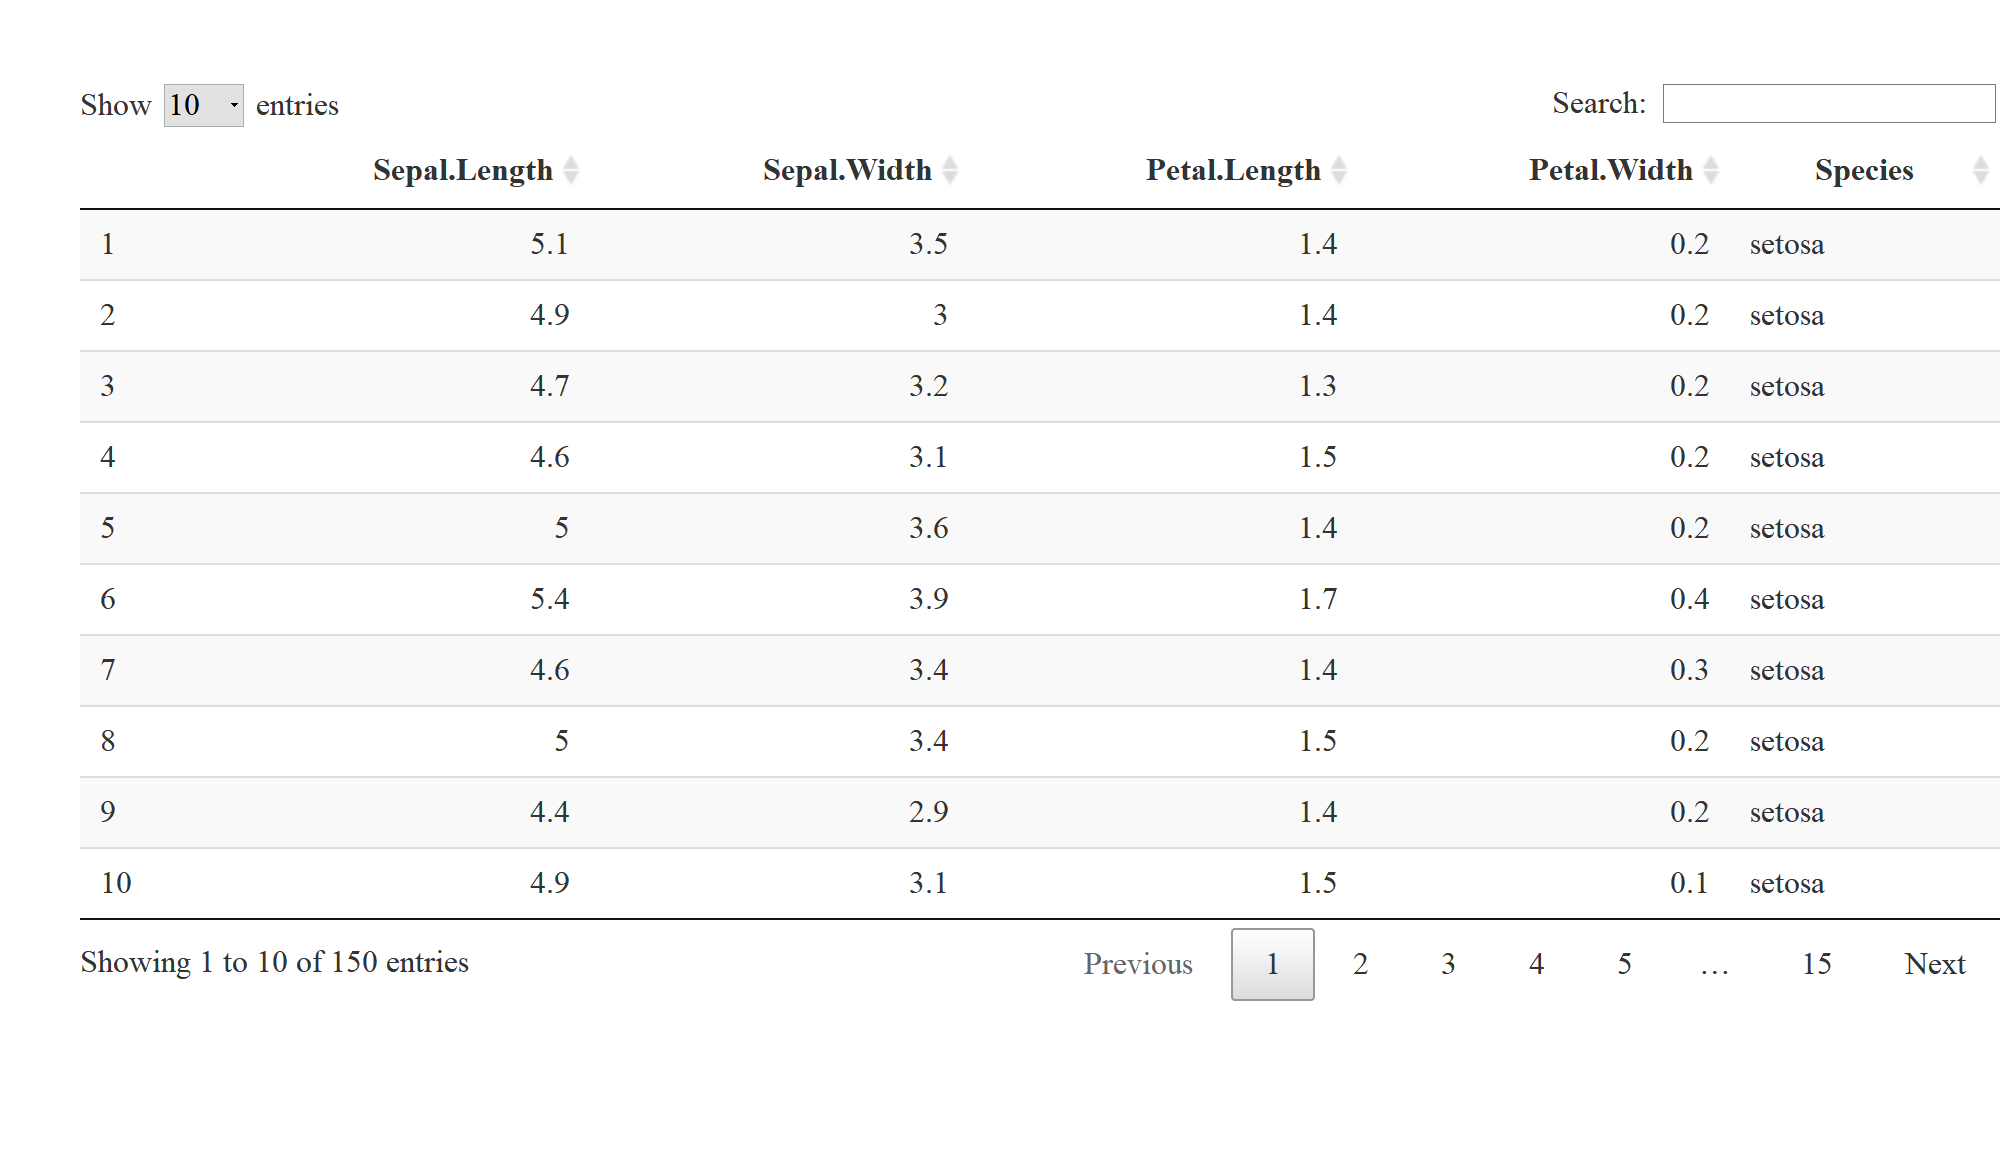
\includegraphics{bookdown-book-zhCN_files/figure-latex/DT-demo-1.png}
\caption{\label{fig:DT-demo}A table widget rendered via the DT package.}
\end{figure}

If you are reading this book as web pages now, you should see an interactive table generated from the above code chunk, e.g., you may sort the columns and search in the table. If you are reading a non-HTML version of this book, you should see a screenshot of the table. The screenshot may look a little different with the actual widget rendered in the web browser, due to the difference between a real web browser and PhantomJS's virtual browser.

There are a number of \textbf{knitr} chunk options related to screen-capturing. First, if you are not satisfied with the quality of the automatic screenshots, or want a screenshot of the widget of a particular state (e.g., after you click and sort a certain column of a table), you may capture the screen manually, and provide your own screenshot via the chunk option \texttt{screenshot.alt} (alternative screenshots). This option takes the paths of images. If you have multiple widgets in a chunk, you can provide a vector of image paths. When this option is present, \textbf{knitr} will no longer call \textbf{webshot} to take automatic screenshots.

Second, sometimes you may want to force \textbf{knitr} to use static screenshots instead of rendering the actual widgets even on HTML pages. In this case, you can set the chunk option \texttt{screenshot.force\ =\ TRUE}, and widgets will always be rendered as static images. Note that you can still choose to use automatic or custom screenshots.

Third, \textbf{webshot} has some options to control the automatic screenshots, and you may specify these options via the chunk option \texttt{screenshot.opts}, which takes a list like \texttt{list(delay\ =\ 2,\ cliprect\ =\ \textquotesingle{}viewport\textquotesingle{})}. See the help page \texttt{?webshot::webshot} for the full list of possible options, and the \href{https://cran.rstudio.com/web/packages/webshot/vignettes/intro.html}{package vignette} \texttt{vignette(\textquotesingle{}intro\textquotesingle{},\ package\ =\ \textquotesingle{}webshot\textquotesingle{})} illustrates the effect of these options. Here the \texttt{delay} option can be important for widgets that take long time to render: \texttt{delay} specifies the number of seconds to wait before PhantomJS takes the screenshot. If you see an incomplete screenshot, you may want to specify a longer delay (the default is 0.2 seconds).

Fourth, if you feel it is slow to capture the screenshots, or do not want to do it every time the code chunk is executed, you may use the chunk option \texttt{cache\ =\ TRUE} to cache the chunk. Caching works for both HTML and non-HTML output formats.

Screenshots behave like normal R plots in the sense that many chunk options related to figures also apply to screenshots, including \texttt{fig.width}, \texttt{fig.height}, \texttt{out.width}, \texttt{fig.cap}, and so on. So you can specify the size of screenshots in the output document, and assign figure captions to them as well. The image format of the automatic screenshots can be specified via the chunk option \texttt{dev}, and possible values are \texttt{pdf}, \texttt{png}, and \texttt{jpeg}. The default for PDF output is \texttt{pdf}, and it is \texttt{png} for other types of output. Note that \texttt{pdf} may not work as faithfully as \texttt{png}: sometimes there are certain elements on an HTML page that fail to render to the PDF screenshot, so you may want to use \texttt{dev\ =\ \textquotesingle{}png\textquotesingle{}} even for PDF output. It depends on specific cases of HTML widgets, and you can try both \texttt{pdf} and \texttt{png} (or \texttt{jpeg}) before deciding which format is more desirable.

\hypertarget{web-pages-and-shiny-apps}{%
\section{Web pages and Shiny apps}\label{web-pages-and-shiny-apps}}

Similar to HTML widgets, arbitrary web pages can be embedded in the book. You can use the function \texttt{knitr::include\_url()} to include a web page through its URL. When the output format is HTML, an \texttt{iframe} is used;\footnote{An \texttt{iframe} is basically a box on one web page to embed another web page.} in other cases, \textbf{knitr} tries to take a screenshot of the web page (or use the custom screenshot you provided). All chunk options are the same as those for HTML widgets. One option that may require your special attention is the \texttt{delay} option: HTML widgets are rendered locally, so usually they are fast to load for PhantomJS to take screenshots, but an arbitrary URL may take longer to load, so you may want to use a larger \texttt{delay} value, e.g., use the chunk option \texttt{screenshot.opts\ =\ list(delay\ =\ 5)}.

A related function is \texttt{knitr::include\_app()}, which is very similar to \texttt{include\_url()}, and it was designed for embedding Shiny apps\index{Shiny application} via their URLs in the output. Its only difference with \texttt{include\_url()} is that it automatically adds a query parameter \texttt{?showcase=0} to the URL, if no other query parameters are present in the URL, to disable the Shiny showcase mode, which is unlikely to be useful for screenshots or iframes. If you do want the showcase mode, use \texttt{include\_url()} instead of \texttt{include\_app()}. Below is a Shiny app example (Figure \ref{fig:miniUI}):

\let\ooldhref\href
\let\href\oldhref

\begin{Shaded}
\begin{Highlighting}[]
\NormalTok{knitr}\SpecialCharTok{::}\FunctionTok{include\_app}\NormalTok{(}\StringTok{\textquotesingle{}https://yihui.shinyapps.io/miniUI/\textquotesingle{}}\NormalTok{, }\AttributeTok{height =} \StringTok{\textquotesingle{}600px\textquotesingle{}}\NormalTok{)}
\end{Highlighting}
\end{Shaded}

\begin{figure}

{\centering \oldhref{https://yihui.shinyapps.io/miniUI/}{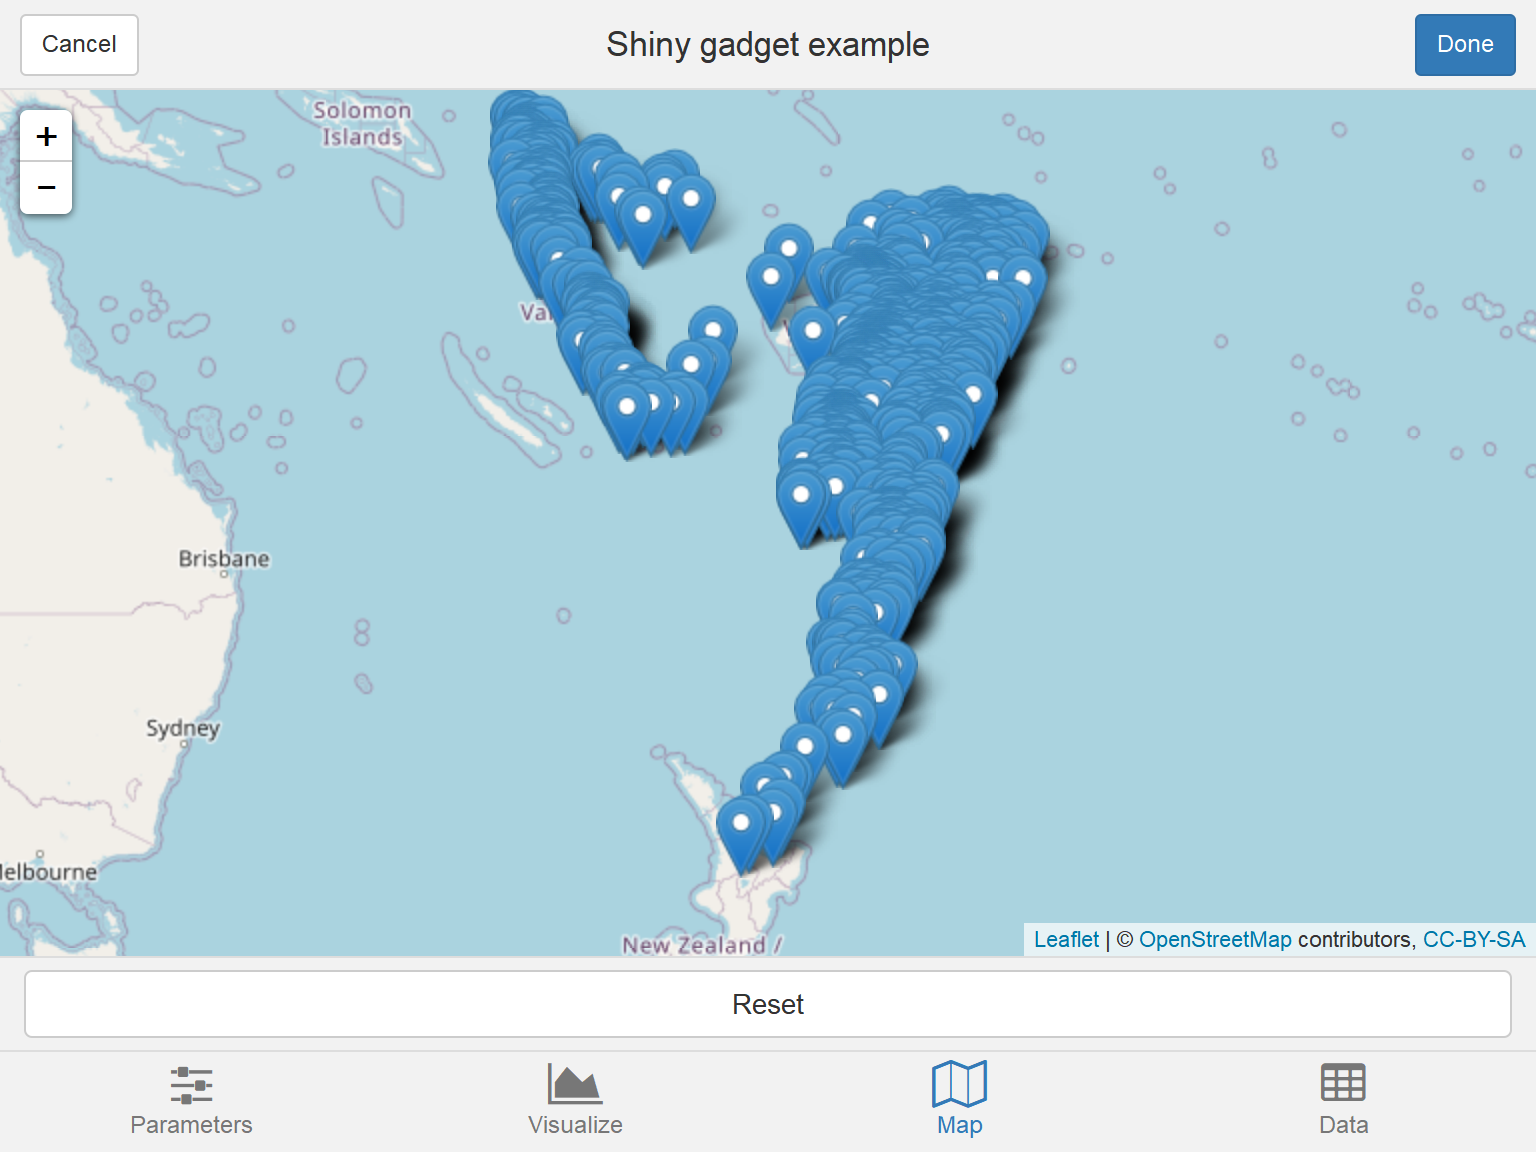
\includegraphics{bookdown-book-zhCN_files/figure-latex/miniUI-1} }

}

\caption{A Shiny app created via the miniUI package; you can see a live version at https://yihui.shinyapps.io/miniUI/.}\label{fig:miniUI}
\end{figure}

\let\href\ooldhref

Again, you will see a live app if you are reading an HTML version of this book, and a static screenshot if you are reading other types of formats. The above Shiny app was created using the \textbf{miniUI} package \citep{R-miniUI}, which provides layout functions that are particularly nice for Shiny apps on small screens. If you use normal Shiny layout functions, you are likely to see vertical and/or horizontal scrollbars in the iframes because the page size is too big to fit in an iframe. When the default width of the iframe is too small, you may use the chunk option \texttt{out.width} to change it. For the height of the iframe, use the \texttt{height} argument of \texttt{include\_url()}/\texttt{include\_app()}.

Shiny apps may take even longer to load than usual URLs. You may want to use a conservative value for the \texttt{delay} option, e.g., 10. Needless to say, \texttt{include\_url()} and \texttt{include\_app()} require a working Internet connection, unless you have previously cached the chunk (but web pages inside iframes still will not work without an Internet connection).

\hypertarget{output-formats}{%
\chapter{Output Formats}\label{output-formats}}

The \textbf{bookdown} package primarily supports three types of output formats: HTML, LaTeX/PDF, and e-books. In this chapter, we introduce the possible options for these formats. Output formats can be specified either in the YAML metadata of the first Rmd file of the book, or in a separate YAML file named \texttt{\_output.yml} under the root directory of the book. Here is a brief example of the former (output formats are specified in the \texttt{output} field of the YAML metadata):

\begin{Shaded}
\begin{Highlighting}[]
\PreprocessorTok{{-}{-}{-}}
\FunctionTok{title}\KeywordTok{:}\AttributeTok{ }\StringTok{"An Impressive Book"}
\FunctionTok{author}\KeywordTok{:}\AttributeTok{ }\StringTok{"Li Lei and Han Meimei"}
\FunctionTok{output}\KeywordTok{:}
\AttributeTok{  bookdown:}\FunctionTok{:gitbook}\KeywordTok{:}
\AttributeTok{    }\FunctionTok{lib\_dir}\KeywordTok{:}\AttributeTok{ assets}
\AttributeTok{    }\FunctionTok{split\_by}\KeywordTok{:}\AttributeTok{ section}
\AttributeTok{    }\FunctionTok{config}\KeywordTok{:}
\AttributeTok{      }\FunctionTok{toolbar}\KeywordTok{:}
\AttributeTok{        }\FunctionTok{position}\KeywordTok{:}\AttributeTok{ static}
\AttributeTok{  bookdown:}\FunctionTok{:pdf\_book}\KeywordTok{:}
\AttributeTok{    }\FunctionTok{keep\_tex}\KeywordTok{:}\AttributeTok{ }\CharTok{yes}
\AttributeTok{  bookdown:}\FunctionTok{:html\_book}\KeywordTok{:}
\AttributeTok{    }\FunctionTok{css}\KeywordTok{:}\AttributeTok{ toc.css}
\FunctionTok{documentclass}\KeywordTok{:}\AttributeTok{ book}
\PreprocessorTok{{-}{-}{-}}
\end{Highlighting}
\end{Shaded}

Here is an example of \texttt{\_output.yml}\index{\_output.yml}:

\begin{Shaded}
\begin{Highlighting}[]
\AttributeTok{bookdown:}\FunctionTok{:gitbook}\KeywordTok{:}
\AttributeTok{  }\FunctionTok{lib\_dir}\KeywordTok{:}\AttributeTok{ assets}
\AttributeTok{  }\FunctionTok{split\_by}\KeywordTok{:}\AttributeTok{ section}
\AttributeTok{  }\FunctionTok{config}\KeywordTok{:}
\AttributeTok{    }\FunctionTok{toolbar}\KeywordTok{:}
\AttributeTok{      }\FunctionTok{position}\KeywordTok{:}\AttributeTok{ static}
\AttributeTok{bookdown:}\FunctionTok{:pdf\_book}\KeywordTok{:}
\AttributeTok{  }\FunctionTok{keep\_tex}\KeywordTok{:}\AttributeTok{ }\CharTok{yes}
\AttributeTok{bookdown:}\FunctionTok{:html\_book}\KeywordTok{:}
\AttributeTok{  }\FunctionTok{css}\KeywordTok{:}\AttributeTok{ toc.css}
\end{Highlighting}
\end{Shaded}

In this case, all formats should be at the top level, instead of under an \texttt{output} field. You do not need the three dashes \texttt{-\/-\/-} in \texttt{\_output.yml}.

\hypertarget{html}{%
\section{HTML}\label{html}}

The main difference between rendering a book (using \textbf{bookdown}) with rendering a single R Markdown document (using \textbf{rmarkdown}) to HTML\index{HTML} is that a book will generate multiple HTML pages by default --- normally one HTML file per chapter. This makes it easier to bookmark a certain chapter or share its URL with others as you read the book, and faster to load a book into the web browser. Currently we have provided a number of different styles for HTML output: the GitBook style, the Bootstrap style, and the Tufte style.

\hypertarget{gitbook-style}{%
\subsection{GitBook style}\label{gitbook-style}}

The GitBook style was borrowed from GitBook\index{GitBook}, a project launched by Friendcode, Inc.~(\url{https://www.gitbook.com}) and dedicated to helping authors write books with Markdown. It provides a beautiful style, with a layout consisting of a sidebar showing the table of contents on the left, and the main body of a book on the right. The design is responsive to the window size, e.g., the navigation buttons are displayed on the left/right of the book body when the window is wide enough, and collapsed into the bottom when the window is narrow to give readers more horizontal space to read the book body.

We have made several improvements over the original GitBook project. The most significant one is that we replaced the Markdown engine with R Markdown v2 based on Pandoc, so that there are a lot more features for you to use when writing a book:

\begin{itemize}
\tightlist
\item
  You can embed R code chunks and inline R expressions in Markdown, and this makes it easy to create reproducible documents and frees you from synchronizing your computation with its actual output (\textbf{knitr} will take care of it automatically).
\item
  The Markdown syntax is much richer: you can write anything that Pandoc's Markdown supports, such as LaTeX math expressions and citations.
\item
  You can embed interactive content in the book (for HTML output only), such as HTML widgets and Shiny apps.
\end{itemize}

We have also added some useful features in the user interface that we will introduce in detail soon. The output format function for the GitBook style in \textbf{bookdown} is \texttt{gitbook()}. Here are its arguments:

\begin{Shaded}
\begin{Highlighting}[]
\FunctionTok{gitbook}\NormalTok{(}\AttributeTok{fig\_caption =} \ConstantTok{TRUE}\NormalTok{, }\AttributeTok{number\_sections =} \ConstantTok{TRUE}\NormalTok{,}
  \AttributeTok{self\_contained =} \ConstantTok{FALSE}\NormalTok{, }\AttributeTok{anchor\_sections =} \ConstantTok{TRUE}\NormalTok{,}
  \AttributeTok{lib\_dir =} \StringTok{"libs"}\NormalTok{, }\AttributeTok{pandoc\_args =} \ConstantTok{NULL}\NormalTok{, ...,}
  \AttributeTok{template =} \StringTok{"default"}\NormalTok{,}
  \AttributeTok{split\_by =} \FunctionTok{c}\NormalTok{(}\StringTok{"chapter"}\NormalTok{, }\StringTok{"chapter+number"}\NormalTok{, }\StringTok{"section"}\NormalTok{, }\StringTok{"section+number"}\NormalTok{, }\StringTok{"rmd"}\NormalTok{, }\StringTok{"none"}\NormalTok{),}
  \AttributeTok{split\_bib =} \ConstantTok{TRUE}\NormalTok{, }\AttributeTok{config =} \FunctionTok{list}\NormalTok{(), }\AttributeTok{table\_css =} \ConstantTok{TRUE}\NormalTok{)}
\end{Highlighting}
\end{Shaded}

Most arguments are passed to \texttt{rmarkdown::html\_document()}, including \texttt{fig\_caption}, \texttt{lib\_dir}, and \texttt{...}. You can check out the help page of \texttt{rmarkdown::html\_document()} for the full list of possible options. We strongly recommend you to use \texttt{fig\_caption\ =\ TRUE} for two reasons: 1) it is important to explain your figures with captions; 2) enabling figure captions means figures will be placed in floating environments when the output is LaTeX, otherwise you may end up with a lot of white space on certain pages. The format of figure/table numbers depends on if sections are numbered or not: if \texttt{number\_sections\ =\ TRUE}, these numbers will be of the format \texttt{X.i}, where \texttt{X} is the chapter number, and \texttt{i} in an incremental number; if sections are not numbered, all figures/tables will be numbered sequentially through the book from 1, 2, \ldots, N. Note that in either case, figures and tables will be numbered independently.

Among all possible arguments in \texttt{...}, you are most likely to use the \texttt{css} argument to provide one or more custom CSS files to tweak the default CSS style. There are a few arguments of \texttt{html\_document()} that have been hard-coded in \texttt{gitbook()} and you cannot change them: \texttt{toc\ =\ TRUE} (there must be a table of contents), \texttt{theme\ =\ NULL} (not using any Bootstrap themes), and \texttt{template} (there exists an internal GitBook template).

Please note that if you change \texttt{self\_contained\ =\ TRUE} to make self-contained HTML pages, the total size of all HTML files can be significantly increased since there are many JS and CSS files that have to be embedded in every single HTML file.

Besides these \texttt{html\_document()} options, \texttt{gitbook()} has three other arguments: \texttt{split\_by}, \texttt{split\_bib}, and \texttt{config}. The \texttt{split\_by} argument specifies how you want to split the HTML output into multiple pages, and its possible values are:

\begin{itemize}
\tightlist
\item
  \texttt{rmd}: use the base filenames of the input Rmd files to create the HTML filenames, e.g., generate \texttt{chapter3.html} for \texttt{chapter3.Rmd}.
\item
  \texttt{none}: do not split the HTML file (the book will be a single HTML file).
\item
  \texttt{chapter}: split the file by the first-level headers.
\item
  \texttt{section}: split the file by the second-level headers.
\item
  \texttt{chapter+number} and \texttt{section+number}: similar to \texttt{chapter} and \texttt{section}, but the files will be numbered.
\end{itemize}

For \texttt{chapter} and \texttt{section}, the HTML filenames will be determined by the header identifiers, e.g., the filename for the first chapter with a chapter title \texttt{\#\ Introduction} will be \texttt{introduction.html} by default. For \texttt{chapter+number} and \texttt{section+number}, the chapter/section numbers will be prepended to the HTML filenames, e.g., \texttt{1-introduction.html} and \texttt{2-1-literature.html}. The header identifier is automatically generated from the header text by default,\footnote{To see more details on how an identifier is automatically generated, see the \texttt{auto\_identifiers} extension in Pandoc's documentation \url{http://pandoc.org/MANUAL.html\#header-identifiers}} and you can manually specify an identifier using the syntax \texttt{\{\#your-custom-id\}} after the header text, e.g.,

\begin{Shaded}
\begin{Highlighting}[]
\FunctionTok{\# An Introduction \{\#introduction\}}

\NormalTok{The default identifier is }\InformationTok{\textasciigrave{}an{-}introduction\textasciigrave{}}\NormalTok{ but we changed}
\NormalTok{it to }\InformationTok{\textasciigrave{}introduction\textasciigrave{}}\NormalTok{.}
\end{Highlighting}
\end{Shaded}

By default, the bibliography is split and relevant citation items are put at the bottom of each page, so that readers do not have to navigate to a different bibliography page to see the details of citations. This feature can be disabled using \texttt{split\_bib\ =\ FALSE}, in which case all citations are put on a separate page.

There are several sub-options in the \texttt{config} option for you to tweak some details in the user interface. Recall that all output format options (not only for \texttt{bookdown::gitbook}) can be either passed to the format function if you use the command-line interface \texttt{bookdown::render\_book()}, or written in the YAML metadata. We display the default sub-options of \texttt{config} in the \texttt{gitbook} format as YAML metadata below (note that they are indented under the \texttt{config} option):

\begin{Shaded}
\begin{Highlighting}[]
\AttributeTok{bookdown:}\FunctionTok{:gitbook}\KeywordTok{:}
\AttributeTok{  }\FunctionTok{config}\KeywordTok{:}
\AttributeTok{    }\FunctionTok{toc}\KeywordTok{:}
\AttributeTok{      }\FunctionTok{collapse}\KeywordTok{:}\AttributeTok{ subsection}
\AttributeTok{      }\FunctionTok{scroll\_highlight}\KeywordTok{:}\AttributeTok{ }\CharTok{yes}
\AttributeTok{      }\FunctionTok{before}\KeywordTok{:}\AttributeTok{ }\CharTok{null}
\AttributeTok{      }\FunctionTok{after}\KeywordTok{:}\AttributeTok{ }\CharTok{null}
\AttributeTok{    }\FunctionTok{toolbar}\KeywordTok{:}
\AttributeTok{      }\FunctionTok{position}\KeywordTok{:}\AttributeTok{ fixed}
\AttributeTok{    }\FunctionTok{edit }\KeywordTok{:}\AttributeTok{ }\CharTok{null}
\AttributeTok{    }\FunctionTok{download}\KeywordTok{:}\AttributeTok{ }\CharTok{null}
\AttributeTok{    }\FunctionTok{search}\KeywordTok{:}
\AttributeTok{      }\FunctionTok{engine}\KeywordTok{:}\AttributeTok{ lunr}\CommentTok{ \# or fuse}
\CommentTok{      \# options to control/tune search engine behaviour (for}
\CommentTok{      \# fuse.js, refer to https://fusejs.io/api/options.html)}
\AttributeTok{      }\FunctionTok{options}\KeywordTok{:}\AttributeTok{ }\CharTok{null}
\AttributeTok{    }\FunctionTok{fontsettings}\KeywordTok{:}
\AttributeTok{      }\FunctionTok{theme}\KeywordTok{:}\AttributeTok{ white}
\AttributeTok{      }\FunctionTok{family}\KeywordTok{:}\AttributeTok{ sans}
\AttributeTok{      }\FunctionTok{size}\KeywordTok{:}\AttributeTok{ }\DecValTok{2}
\AttributeTok{    }\FunctionTok{sharing}\KeywordTok{:}
\AttributeTok{      }\FunctionTok{facebook}\KeywordTok{:}\AttributeTok{ }\CharTok{yes}
\AttributeTok{      }\FunctionTok{github}\KeywordTok{:}\AttributeTok{ }\CharTok{no}
\AttributeTok{      }\FunctionTok{twitter}\KeywordTok{:}\AttributeTok{ }\CharTok{yes}
\AttributeTok{      }\FunctionTok{linkedin}\KeywordTok{:}\AttributeTok{ }\CharTok{no}
\AttributeTok{      }\FunctionTok{weibo}\KeywordTok{:}\AttributeTok{ }\CharTok{no}
\AttributeTok{      }\FunctionTok{instapaper}\KeywordTok{:}\AttributeTok{ }\CharTok{no}
\AttributeTok{      }\FunctionTok{vk}\KeywordTok{:}\AttributeTok{ }\CharTok{no}
\AttributeTok{      }\FunctionTok{whatsapp}\KeywordTok{:}\AttributeTok{ }\CharTok{no}
\AttributeTok{      }\FunctionTok{all}\KeywordTok{:}\AttributeTok{ }\KeywordTok{[}\StringTok{\textquotesingle{}facebook\textquotesingle{}}\KeywordTok{,}\AttributeTok{ }\StringTok{\textquotesingle{}twitter\textquotesingle{}}\KeywordTok{,}\AttributeTok{ }\StringTok{\textquotesingle{}linkedin\textquotesingle{}}\KeywordTok{,}\AttributeTok{ }\StringTok{\textquotesingle{}weibo\textquotesingle{}}\KeywordTok{,}\AttributeTok{ }\StringTok{\textquotesingle{}instapaper\textquotesingle{}}\KeywordTok{]}
\AttributeTok{    }\FunctionTok{info}\KeywordTok{:}\AttributeTok{ }\CharTok{yes}
\end{Highlighting}
\end{Shaded}

The \texttt{toc} option controls the behavior of the table of contents (TOC). You can collapse some items initially when a page is loaded via the \texttt{collapse} option. Its possible values are \texttt{subsection}, \texttt{section}, \texttt{none} (or \texttt{null}). This option can be helpful if your TOC is very long and has more than three levels of headings: \texttt{subsection} means collapsing all TOC items for subsections (X.X.X), \texttt{section} means those items for sections (X.X) so only the top-level headings are displayed initially, and \texttt{none} means not collapsing any items in the TOC. For those collapsed TOC items, you can toggle their visibility by clicking their parent TOC items. For example, you can click a chapter title in the TOC to show/hide its sections.

The \texttt{scroll\_highlight} option in \texttt{toc} indicates whether to enable highlighting of TOC items as you scroll the book body (by default this feature is enabled). Whenever a new header comes into the current viewport as you scroll down/up, the corresponding item in TOC on the left will be highlighted.

Since the sidebar has a fixed width, when an item in the TOC is truncated because the heading text is too wide, you can hover the cursor over it to see a tooltip showing the full text.

You may add more items before and after the TOC using the HTML tag \texttt{\textless{}li\textgreater{}}. These items will be separated from the TOC using a horizontal divider. You can use the pipe character \texttt{\textbar{}} so that you do not need to escape any characters in these items following the YAML syntax, e.g.,

\begin{verbatim}
    toc:
      before: |
        <li><a href="...">My Awesome Book</a></li>
        <li><a href="...">John Smith</a></li>
      after: |
        <li><a href="https://github.com/rstudio/bookdown">
        Proudly published with bookdown</a></li>
\end{verbatim}

As you navigate through different HTML pages, we will try to preserve the scroll position of the TOC. Normally you will see the scrollbar in the TOC at a fixed position even if you navigate to the next page. However, if the TOC item for the current chapter/section is not visible when the page is loaded, we will automatically scroll the TOC to make it visible to you.

\begin{figure}

\includegraphics[width=1\linewidth]{images/gitbook} \caption{The GitBook toolbar.}\label{fig:gitbook-toolbar}
\end{figure}

The GitBook style has a toolbar (Figure \ref{fig:gitbook-toolbar}) at the top of each page that allows you to dynamically change the book settings. The \texttt{toolbar} option has a sub-option \texttt{position}, which can take values \texttt{fixed} or \texttt{static}. The default is that the toolbar will be fixed at the top of the page, so even if you scroll down the page, the toolbar is still visible there. If it is \texttt{static}, the toolbar will not scroll with the page, i.e., once you scroll away, you will no longer see it.

The first button on the toolbar can toggle the visibility of the sidebar. You can also hit the \texttt{S} key on your keyboard to do the same thing. The GitBook style can remember the visibility status of the sidebar, e.g., if you closed the sidebar, it will remain closed the next time you open the book. In fact, the GitBook style remembers many other settings as well, such as the search keyword and the font settings.

The second button on the toolbar is the search button. Its keyboard shortcut is \texttt{F} (Find). When the button is clicked, you will see a search box at the top of the sidebar. As you type in the box, the TOC will be filtered to display the sections that match the search keyword. Now you can use the arrow keys \texttt{Up}/\texttt{Down} to highlight the previous/next match in the search results. When you click the search button again (or hit \texttt{F} outside the search box), the search keyword will be emptied and the search box will be hidden. To disable searching, set the option \texttt{search:\ no} in \texttt{config}.

The third button is for font/theme settings. The reader can change the font size (bigger or smaller), the font family (serif or sans serif), and the theme (\texttt{White}, \texttt{Sepia}, or \texttt{Night}). You can set the initial value of these settings via the \texttt{fontsettings} option. Font size is measured on a scale of 0-4; the initial value can be set to 1, 2 (default), 3, or 4. The button can be removed from the toolbar by setting \texttt{fontsettings:\ null} (or \texttt{no}).

\begin{Shaded}
\begin{Highlighting}[]
\CommentTok{\# changing the default}
\AttributeTok{    }\FunctionTok{fontsettings}\KeywordTok{:}
\AttributeTok{      }\FunctionTok{theme}\KeywordTok{:}\AttributeTok{ night}
\AttributeTok{      }\FunctionTok{family}\KeywordTok{:}\AttributeTok{ serif}
\AttributeTok{      }\FunctionTok{size}\KeywordTok{:}\AttributeTok{ }\DecValTok{3}
\end{Highlighting}
\end{Shaded}

The \texttt{edit} option is the same as the option mentioned in Section \ref{configuration}. If it is not empty, an edit button will be added to the toolbar. This was designed for potential contributors to the book to contribute by editing the book on GitHub after clicking the button and sending pull requests. The \texttt{history} and \texttt{view} options work the same
way.

If your book has other output formats for readers to download, you may provide the \texttt{download} option so that a download button can be added to the toolbar. This option takes either a character vector, or a list of character vectors with the length of each vector being 2. When it is a character vector, it should be either a vector of filenames, or filename extensions, e.g., both of the following settings are okay:

\begin{Shaded}
\begin{Highlighting}[]
\AttributeTok{    }\FunctionTok{download}\KeywordTok{:}\AttributeTok{ }\KeywordTok{[}\StringTok{"book.pdf"}\KeywordTok{,}\AttributeTok{ }\StringTok{"book.epub"}\KeywordTok{]}
\AttributeTok{    }\FunctionTok{download}\KeywordTok{:}\AttributeTok{ }\KeywordTok{[}\StringTok{"pdf"}\KeywordTok{,}\AttributeTok{ }\StringTok{"epub"}\KeywordTok{,}\AttributeTok{ }\StringTok{"mobi"}\KeywordTok{]}
\end{Highlighting}
\end{Shaded}

When you only provide the filename extensions, the filename is derived from the book filename of the configuration file \texttt{\_bookdown.yml} (Section \ref{configuration}). When \texttt{download} is \texttt{null}, \texttt{gitbook()} will look for PDF, EPUB, and MOBI files in the book output directory, and automatically add them to the \texttt{download} option. If you just want to suppress the download button, use \texttt{download:\ no}. All files for readers to download will be displayed in a drop-down menu, and the filename extensions are used as the menu text. When the only available format for readers to download is PDF, the download button will be a single PDF button instead of a drop-down menu.

An alternative form for the value of the \texttt{download} option is a list of length-2 vectors, e.g.,

\begin{Shaded}
\begin{Highlighting}[]
\AttributeTok{    }\FunctionTok{download}\KeywordTok{:}\AttributeTok{ }\KeywordTok{[[}\StringTok{"book.pdf"}\KeywordTok{,}\AttributeTok{ }\StringTok{"PDF"}\KeywordTok{],}\AttributeTok{ }\KeywordTok{[}\StringTok{"book.epub"}\KeywordTok{,}\AttributeTok{ }\StringTok{"EPUB"}\KeywordTok{]]}
\end{Highlighting}
\end{Shaded}

You can also write it as:

\begin{Shaded}
\begin{Highlighting}[]
\AttributeTok{    }\FunctionTok{download}\KeywordTok{:}
\AttributeTok{      }\KeywordTok{{-}}\AttributeTok{ }\KeywordTok{[}\StringTok{"book.pdf"}\KeywordTok{,}\AttributeTok{ }\StringTok{"PDF"}\KeywordTok{]}
\AttributeTok{      }\KeywordTok{{-}}\AttributeTok{ }\KeywordTok{[}\StringTok{"book.epub"}\KeywordTok{,}\AttributeTok{ }\StringTok{"EPUB"}\KeywordTok{]}
\end{Highlighting}
\end{Shaded}

Each vector in the list consists of the filename and the text to be displayed in the menu. Compared to the first form, this form allows you to customize the menu text, e.g., you may have two different copies of the PDF for readers to download and you will need to make the menu items different.

On the right of the toolbar, there are some buttons to share the link on social network websites such as Twitter, Facebook, and Linkedin. You can use the \texttt{sharing} option to decide which buttons to enable. If you want to get rid of these buttons entirely, use \texttt{sharing:\ null} (or \texttt{no}).

Another button shown on the toolbar is the information (`i') button that lists keyboard shortcuts available to navigate the document. This button can be hidden by setting \texttt{info:\ no}.

Finally, there are a few more top-level options in the YAML metadata that can be passed to the GitBook HTML template via Pandoc. They may not have clear visible effects on the HTML output, but they may be useful when you deploy the HTML output as a website. These options include:

\begin{itemize}
\tightlist
\item
  \texttt{description}: A character string to be written to the \texttt{content} attribute of the tag \texttt{\textless{}meta\ name="description"\ content=""\textgreater{}} in the HTML head (if missing, the title of the book will be used). This can be useful for search engine optimization (SEO). Note that it should be plain text without any Markdown formatting such as \texttt{\_italic\_} or \texttt{**bold**}.
\item
  \texttt{url}: The URL of book's website, e.g., \texttt{https\textbackslash{}://bookdown.org/yihui/bookdown/}.\footnote{The backslash before \texttt{:} is due to a technical issue: we want to prevent Pandoc from translating the link to HTML code \texttt{\textless{}a\ href="..."\textgreater{}\textless{}/a\textgreater{}}. More details at \url{https://github.com/jgm/pandoc/issues/2139}.}
\item
  \texttt{github-repo}: The GitHub repository of the book of the form \texttt{user/repo}.
\item
  \texttt{cover-image}: The path to the cover image of the book.
\item
  \texttt{apple-touch-icon}: A path to an icon (e.g., a PNG image). This is for iOS only: when the website is added to the Home screen, the link is represented by this icon.
\item
  \texttt{apple-touch-icon-size}: The size of the icon (by default, 152 x 152 pixels).
\item
  \texttt{favicon}: A path to the ``favorite icon''. Typically this icon is displayed in the browser's address bar, or in front of the page title on the tab if the browser support tabs.
\end{itemize}

Below we show some sample YAML metadata (again, please note that these are \emph{top-level} options):

\begin{Shaded}
\begin{Highlighting}[]
\PreprocessorTok{{-}{-}{-}}
\FunctionTok{title}\KeywordTok{:}\AttributeTok{ }\StringTok{"An Awesome Book"}
\FunctionTok{author}\KeywordTok{:}\AttributeTok{ }\StringTok{"John Smith"}
\FunctionTok{description}\KeywordTok{:}\AttributeTok{ }\StringTok{"This book introduces the ABC theory, and ..."}
\FunctionTok{url}\KeywordTok{:}\AttributeTok{ }\StringTok{\textquotesingle{}https\textbackslash{}://bookdown.org/john/awesome/\textquotesingle{}}
\FunctionTok{github{-}repo}\KeywordTok{:}\AttributeTok{ }\StringTok{"john/awesome"}
\FunctionTok{cover{-}image}\KeywordTok{:}\AttributeTok{ }\StringTok{"images/cover.png"}
\FunctionTok{apple{-}touch{-}icon}\KeywordTok{:}\AttributeTok{ }\StringTok{"touch{-}icon.png"}
\FunctionTok{apple{-}touch{-}icon{-}size}\KeywordTok{:}\AttributeTok{ }\DecValTok{120}
\FunctionTok{favicon}\KeywordTok{:}\AttributeTok{ }\StringTok{"favicon.ico"}
\PreprocessorTok{{-}{-}{-}}
\end{Highlighting}
\end{Shaded}

A nice effect of setting \texttt{description} and \texttt{cover-image} is that when you share the link of your book on some social network websites such as Twitter, the link can be automatically expanded to a card with the cover image and description of the book.

\hypertarget{bootstrap-style}{%
\subsection{Bootstrap style}\label{bootstrap-style}}

If you have used R Markdown before, you should be familiar with the Bootstrap\index{Bootstrap style} style (\url{http://getbootstrap.com}), which is the default style of the HTML output of R Markdown. The output format function in \textbf{rmarkdown} is \texttt{html\_document()}, and we have a corresponding format \texttt{html\_book()} in \textbf{bookdown} using \texttt{html\_document()} as the base format. In fact, there is a more general format \texttt{html\_chapters()} in \textbf{bookdown} and \texttt{html\_book()} is just its special case:

\begin{Shaded}
\begin{Highlighting}[]
\FunctionTok{html\_chapters}\NormalTok{(}\AttributeTok{toc =} \ConstantTok{TRUE}\NormalTok{, }\AttributeTok{number\_sections =} \ConstantTok{TRUE}\NormalTok{,}
  \AttributeTok{fig\_caption =} \ConstantTok{TRUE}\NormalTok{, }\AttributeTok{lib\_dir =} \StringTok{"libs"}\NormalTok{,}
  \AttributeTok{template =} \FunctionTok{bookdown\_file}\NormalTok{(}\StringTok{"templates/default.html"}\NormalTok{),}
  \AttributeTok{pandoc\_args =} \ConstantTok{NULL}\NormalTok{, ...,}
  \AttributeTok{base\_format =}\NormalTok{ rmarkdown}\SpecialCharTok{::}\NormalTok{html\_document,}
  \AttributeTok{split\_bib =} \ConstantTok{TRUE}\NormalTok{, }\AttributeTok{page\_builder =}\NormalTok{ build\_chapter,}
  \AttributeTok{split\_by =} \FunctionTok{c}\NormalTok{(}\StringTok{"section+number"}\NormalTok{, }\StringTok{"section"}\NormalTok{, }\StringTok{"chapter+number"}\NormalTok{, }\StringTok{"chapter"}\NormalTok{, }\StringTok{"rmd"}\NormalTok{, }\StringTok{"none"}\NormalTok{))}
\end{Highlighting}
\end{Shaded}

Note that it has a \texttt{base\_format} argument that takes a base output format function, and \texttt{html\_book()} is basically \texttt{html\_chapters(base\_format\ =\ rmarkdown::html\_document)}. All arguments of \texttt{html\_book()} are passed to \texttt{html\_chapters()}:

\begin{Shaded}
\begin{Highlighting}[]
\FunctionTok{html\_book}\NormalTok{(...)}
\end{Highlighting}
\end{Shaded}

That means that you can use most arguments of \texttt{rmarkdown::html\_document}, such as \texttt{toc} (whether to show the table of contents), \texttt{number\_sections} (whether to number section headings), and so on. Again, check the help page of \texttt{rmarkdown::html\_document} to see the full list of possible options. Note that the argument \texttt{self\_contained} is hard-coded to \texttt{FALSE} internally, so you cannot change the value of this argument. We have explained the argument \texttt{split\_by} in the previous section.

The arguments \texttt{template} and \texttt{page\_builder} are for advanced users, and you do not need to understand them unless you have strong need to customize the HTML output, and those many options provided by \texttt{rmarkdown::html\_document()} still do not give you what you want.

If you want to pass a different HTML template to the \texttt{template} argument, the template must contain three pairs of HTML comments, and each comment must be on a separate line:

\begin{itemize}
\tightlist
\item
  \texttt{\textless{}!-\/-bookdown:title:start-\/-\textgreater{}} and \texttt{\textless{}!-\/-bookdown:title:end-\/-\textgreater{}} to mark the title section of the book. This section will be placed only on the first page of the rendered book;
\item
  \texttt{\textless{}!-\/-bookdown:toc:start-\/-\textgreater{}} and \texttt{\textless{}!-\/-bookdown:toc:end-\/-\textgreater{}} to mark the table of contents section, which will be placed on all HTML pages;
\item
  \texttt{\textless{}!-\/-bookdown:body:start-\/-\textgreater{}} and \texttt{\textless{}!-\/-bookdown:body:end-\/-\textgreater{}} to mark the HTML body of the book, and the HTML body will be split into multiple separate pages. Recall that we merge all R Markdown or Markdown files, render them into a single HTML file, and split it.
\end{itemize}

You may open the default HTML template to see where these comments were inserted:

\begin{Shaded}
\begin{Highlighting}[]
\NormalTok{bookdown}\SpecialCharTok{:::}\FunctionTok{bookdown\_file}\NormalTok{(}\StringTok{\textquotesingle{}templates/default.html\textquotesingle{}}\NormalTok{)}
\CommentTok{\# you may use file.edit() to open this file}
\end{Highlighting}
\end{Shaded}

Once you know how \textbf{bookdown} works internally to generate multiple-page HTML output, it will be easier to understand the argument \texttt{page\_builder}, which is a function to compose each individual HTML page using the HTML fragments extracted from the above comment tokens. The default value of \texttt{page\_builder} is a function \texttt{build\_chapter} in \textbf{bookdown}, and its source code is relatively simple (ignore those internal functions like \texttt{button\_link()}):

\begin{Shaded}
\begin{Highlighting}[]
\NormalTok{build\_chapter }\OtherTok{=} \ControlFlowTok{function}\NormalTok{(}
\NormalTok{  head, toc, chapter, link\_prev, link\_next, rmd\_cur, html\_cur, foot}
\NormalTok{) \{}
  \CommentTok{\# add a has{-}sub class to the \textless{}li\textgreater{} items that has sub lists}
\NormalTok{  toc }\OtherTok{=} \FunctionTok{gsub}\NormalTok{(}\StringTok{\textquotesingle{}\^{}(\textless{}li\textgreater{})(.+\textless{}ul\textgreater{})$\textquotesingle{}}\NormalTok{, }\StringTok{\textquotesingle{}\textless{}li class="has{-}sub"\textgreater{}}\SpecialCharTok{\textbackslash{}\textbackslash{}}\StringTok{2\textquotesingle{}}\NormalTok{, toc)}
  \FunctionTok{paste}\NormalTok{(}\FunctionTok{c}\NormalTok{(}
\NormalTok{    head,}
    \StringTok{\textquotesingle{}\textless{}div class="row"\textgreater{}\textquotesingle{}}\NormalTok{,}
    \StringTok{\textquotesingle{}\textless{}div class="col{-}sm{-}12"\textgreater{}\textquotesingle{}}\NormalTok{,}
\NormalTok{    toc,}
    \StringTok{\textquotesingle{}\textless{}/div\textgreater{}\textquotesingle{}}\NormalTok{,}
    \StringTok{\textquotesingle{}\textless{}/div\textgreater{}\textquotesingle{}}\NormalTok{,}
    \StringTok{\textquotesingle{}\textless{}div class="row"\textgreater{}\textquotesingle{}}\NormalTok{,}
    \StringTok{\textquotesingle{}\textless{}div class="col{-}sm{-}12"\textgreater{}\textquotesingle{}}\NormalTok{,}
\NormalTok{    chapter,}
    \StringTok{\textquotesingle{}\textless{}p style="text{-}align: center;"\textgreater{}\textquotesingle{}}\NormalTok{,}
    \FunctionTok{button\_link}\NormalTok{(link\_prev, }\StringTok{\textquotesingle{}Previous\textquotesingle{}}\NormalTok{),}
    \FunctionTok{source\_link}\NormalTok{(rmd\_cur, }\AttributeTok{type =} \StringTok{\textquotesingle{}edit\textquotesingle{}}\NormalTok{),}
    \FunctionTok{source\_link}\NormalTok{(rmd\_cur, }\AttributeTok{type =} \StringTok{\textquotesingle{}history\textquotesingle{}}\NormalTok{),}
    \FunctionTok{source\_link}\NormalTok{(rmd\_cur, }\AttributeTok{type =} \StringTok{\textquotesingle{}view\textquotesingle{}}\NormalTok{),}
    \FunctionTok{button\_link}\NormalTok{(link\_next, }\StringTok{\textquotesingle{}Next\textquotesingle{}}\NormalTok{),}
    \StringTok{\textquotesingle{}\textless{}/p\textgreater{}\textquotesingle{}}\NormalTok{,}
    \StringTok{\textquotesingle{}\textless{}/div\textgreater{}\textquotesingle{}}\NormalTok{,}
    \StringTok{\textquotesingle{}\textless{}/div\textgreater{}\textquotesingle{}}\NormalTok{,}
\NormalTok{    foot}
\NormalTok{  ), }\AttributeTok{collapse =} \StringTok{\textquotesingle{}}\SpecialCharTok{\textbackslash{}n}\StringTok{\textquotesingle{}}\NormalTok{)}
\NormalTok{\}}
\end{Highlighting}
\end{Shaded}

Basically, this function takes a number of components like the HTML head, the table of contents, the chapter body, and so on, and it is expected to return a character string which is the HTML source of a complete HTML page. You may manipulate all components in this function using text-processing functions like \texttt{gsub()} and \texttt{paste()}.

What the default page builder does is to put TOC in the first row, the body in the second row, navigation buttons at the bottom of the body, and concatenate them with the HTML head and foot. Here is a sketch of the HTML source code that may help you understand the output of \texttt{build\_chapter()}:

\begin{Shaded}
\begin{Highlighting}[]
\KeywordTok{\textless{}html\textgreater{}}
  \KeywordTok{\textless{}head\textgreater{}}
    \KeywordTok{\textless{}title\textgreater{}}\NormalTok{A Nice Book}\KeywordTok{\textless{}/title\textgreater{}}
  \KeywordTok{\textless{}/head\textgreater{}}
  \KeywordTok{\textless{}body\textgreater{}}
  
    \KeywordTok{\textless{}div}\OtherTok{ class=}\StringTok{"row"}\KeywordTok{\textgreater{}}\NormalTok{TOC}\KeywordTok{\textless{}/div\textgreater{}}
    
    \KeywordTok{\textless{}div}\OtherTok{ class=}\StringTok{"row"}\KeywordTok{\textgreater{}}
\NormalTok{      CHAPTER BODY}
      \KeywordTok{\textless{}p\textgreater{}}
        \KeywordTok{\textless{}button\textgreater{}}\NormalTok{PREVIOUS}\KeywordTok{\textless{}/button\textgreater{}}
        \KeywordTok{\textless{}button\textgreater{}}\NormalTok{NEXT}\KeywordTok{\textless{}/button\textgreater{}}
      \KeywordTok{\textless{}/p\textgreater{}}
    \KeywordTok{\textless{}/div\textgreater{}}
  
  \KeywordTok{\textless{}/body\textgreater{}}
\KeywordTok{\textless{}/html\textgreater{}}
\end{Highlighting}
\end{Shaded}

For all HTML pages, the main difference is the chapter body, and most of the rest of the elements are the same. The default output from \texttt{html\_book()} will include the Bootstrap CSS and JavaScript files in the \texttt{\textless{}head\textgreater{}} tag.

The TOC is often used for navigation purposes. In the GitBook style, the TOC is displayed in the sidebar. For the Bootstrap style, we did not apply a special style to it, so it is shown as a plain unordered list (in the HTML tag \texttt{\textless{}ul\textgreater{}}). It is easy to turn this list into a navigation bar with some CSS techniques. We have provided a CSS file \texttt{toc.css} in this package that you can use, and you can find it here: \url{https://github.com/rstudio/bookdown/blob/master/inst/examples/css/toc.css}

You may copy this file to the root directory of your book, and apply it to the HTML output via the \texttt{css} option, e.g.,

\begin{Shaded}
\begin{Highlighting}[]
\PreprocessorTok{{-}{-}{-}}
\FunctionTok{output}\KeywordTok{:}
\AttributeTok{  bookdown:}\FunctionTok{:html\_book}\KeywordTok{:}
\AttributeTok{    }\FunctionTok{toc}\KeywordTok{:}\AttributeTok{ }\CharTok{yes}
\AttributeTok{    }\FunctionTok{css}\KeywordTok{:}\AttributeTok{ toc.css}
\PreprocessorTok{{-}{-}{-}}
\end{Highlighting}
\end{Shaded}

There are many possible ways to turn \texttt{\textless{}ul\textgreater{}} lists into navigation menus if you do a little bit searching on the web, and you can choose a menu style that you like. The \texttt{toc.css} we just mentioned is a style with white menu texts on a black background, and supports sub-menus (e.g., section titles are displayed as drop-down menus under chapter titles).

As a matter of fact, you can get rid of the Bootstrap style in \texttt{html\_document()} if you set the \texttt{theme} option to \texttt{null}, and you are free to apply arbitrary styles to the HTML output using the \texttt{css} option (and possibly the \texttt{includes} option if you want to include arbitrary content in the HTML head/foot).

\hypertarget{tufte-style}{%
\subsection{Tufte style}\label{tufte-style}}

Like the Bootstrap style, the Tufte\index{Tufte style} style is provided by an output format \texttt{tufte\_html\_book()}, which is also a special case of \texttt{html\_chapters()} using \texttt{tufte::tufte\_html()} as the base format. Please see the \textbf{tufte} package \citep{R-tufte} if you are not familiar with the Tufte style. Basically, it is a layout with a main column on the left and a margin column on the right. The main body is in the main column, and the margin column is used to place footnotes, margin notes, references, and margin figures, and so on.

All arguments of \texttt{tufte\_html\_book()} have exactly the same meanings as \texttt{html\_book()}, e.g., you can also customize the CSS via the \texttt{css} option. There are a few elements that are specific to the Tufte style, though, such as margin notes, margin figures, and full-width figures. These elements require special syntax to generate; please see the documentation of the \textbf{tufte} package. Note that you do not need to do anything special to footnotes and references (just use the normal Markdown syntax \texttt{\^{}{[}footnote{]}} and \texttt{{[}@citation{]}}), since they will be automatically put in the margin. A brief YAML example of the \texttt{tufte\_html\_book} format:

\begin{Shaded}
\begin{Highlighting}[]
\PreprocessorTok{{-}{-}{-}}
\FunctionTok{output}\KeywordTok{:}
\AttributeTok{  bookdown:}\FunctionTok{:tufte\_html\_book}\KeywordTok{:}
\AttributeTok{    }\FunctionTok{toc}\KeywordTok{:}\AttributeTok{ }\CharTok{yes}
\AttributeTok{    }\FunctionTok{css}\KeywordTok{:}\AttributeTok{ toc.css}
\PreprocessorTok{{-}{-}{-}}
\end{Highlighting}
\end{Shaded}

\hypertarget{latexpdf}{%
\section{LaTeX/PDF}\label{latexpdf}}

We strongly recommend that you use an HTML output format instead of LaTeX\index{LaTeX} when you develop a book, since you will not be too distracted by the typesetting details, which can bother you a lot if you constantly look at the PDF output of a book. Leave the job of careful typesetting to the very end (ideally after you have really finished the content of the book).

The LaTeX/PDF output format is provided by \texttt{pdf\_book()} in \textbf{bookdown}. There is not a significant difference between \texttt{pdf\_book()} and the \texttt{pdf\_document()} format in \textbf{rmarkdown}. The main purpose of \texttt{pdf\_book()} is to resolve the labels and cross-references written using the syntax described in Sections \ref{figures}, \ref{tables}, and \ref{cross-references}. If the only output format that you want for a book is LaTeX/PDF, you may use the syntax specific to LaTeX, such as \texttt{\textbackslash{}label\{\}} to label figures/tables/sections, and \texttt{\textbackslash{}ref\{\}} to cross-reference them via their labels, because Pandoc supports LaTeX commands in Markdown. However, the LaTeX syntax is not portable to other output formats, such as HTML and e-books. That is why we introduced the syntax \texttt{(\textbackslash{}\#label)} for labels and \texttt{\textbackslash{}@ref(label)} for cross-references.

There are some top-level YAML options that will be applied to the LaTeX output. For a book, you may change the default document class to \texttt{book} (the default is \texttt{article}), and specify a bibliography style required by your publisher. A brief YAML example:

\begin{Shaded}
\begin{Highlighting}[]
\PreprocessorTok{{-}{-}{-}}
\FunctionTok{documentclass}\KeywordTok{:}\AttributeTok{ book}
\FunctionTok{bibliography}\KeywordTok{:}\AttributeTok{ }\KeywordTok{[}\AttributeTok{book.bib}\KeywordTok{,}\AttributeTok{ packages.bib}\KeywordTok{]}
\FunctionTok{biblio{-}style}\KeywordTok{:}\AttributeTok{ apalike}
\PreprocessorTok{{-}{-}{-}}
\end{Highlighting}
\end{Shaded}

There are a large number of other YAML options that you can specify for LaTeX output, such as the paper size, font size, page margin, line spacing, font families, and so on. See \url{http://pandoc.org/MANUAL.html\#variables-for-latex} for a full list of options.

The \texttt{pdf\_book()} format is a general format like \texttt{html\_book()}, and it also has a \texttt{base\_format} argument:

\begin{Shaded}
\begin{Highlighting}[]
\FunctionTok{pdf\_book}\NormalTok{(}\AttributeTok{toc =} \ConstantTok{TRUE}\NormalTok{, }\AttributeTok{number\_sections =} \ConstantTok{TRUE}\NormalTok{,}
  \AttributeTok{fig\_caption =} \ConstantTok{TRUE}\NormalTok{, }\AttributeTok{pandoc\_args =} \ConstantTok{NULL}\NormalTok{, ...,}
  \AttributeTok{base\_format =}\NormalTok{ rmarkdown}\SpecialCharTok{::}\NormalTok{pdf\_document,}
  \AttributeTok{toc\_unnumbered =} \ConstantTok{TRUE}\NormalTok{, }\AttributeTok{toc\_appendix =} \ConstantTok{FALSE}\NormalTok{,}
  \AttributeTok{toc\_bib =} \ConstantTok{FALSE}\NormalTok{, }\AttributeTok{quote\_footer =} \ConstantTok{NULL}\NormalTok{,}
  \AttributeTok{highlight\_bw =} \ConstantTok{FALSE}\NormalTok{)}
\end{Highlighting}
\end{Shaded}

You can change the \texttt{base\_format} function to other output format functions, and \textbf{bookdown} has provided a simple wrapper function \texttt{tufte\_book2()}, which is basically \texttt{pdf\_book(base\_format\ =\ tufte::tufte\_book)}, to produce a PDF book using the Tufte PDF style (again, see the \textbf{tufte} package).

\hypertarget{e-books}{%
\section{E-Books}\label{e-books}}

Currently \textbf{bookdown} provides two e-book\index{e-book} formats, EPUB\index{EPUB} and MOBI\index{MOBI}. Books in these formats can be read on devices like smartphones, tablets, or special e-readers such as Kindle.

\hypertarget{epub}{%
\subsection{EPUB}\label{epub}}

To create an EPUB book, you can use the \texttt{epub\_book()} format. It has some options in common with \texttt{rmarkdown::html\_document()}:

\begin{Shaded}
\begin{Highlighting}[]
\FunctionTok{epub\_book}\NormalTok{(}\AttributeTok{fig\_width =} \DecValTok{5}\NormalTok{, }\AttributeTok{fig\_height =} \DecValTok{4}\NormalTok{, }\AttributeTok{dev =} \StringTok{"png"}\NormalTok{,}
  \AttributeTok{fig\_caption =} \ConstantTok{TRUE}\NormalTok{, }\AttributeTok{number\_sections =} \ConstantTok{TRUE}\NormalTok{,}
  \AttributeTok{toc =} \ConstantTok{FALSE}\NormalTok{, }\AttributeTok{toc\_depth =} \DecValTok{3}\NormalTok{, }\AttributeTok{stylesheet =} \ConstantTok{NULL}\NormalTok{,}
  \AttributeTok{cover\_image =} \ConstantTok{NULL}\NormalTok{, }\AttributeTok{metadata =} \ConstantTok{NULL}\NormalTok{,}
  \AttributeTok{chapter\_level =} \DecValTok{1}\NormalTok{, }\AttributeTok{epub\_version =} \FunctionTok{c}\NormalTok{(}\StringTok{"epub3"}\NormalTok{, }\StringTok{"epub"}\NormalTok{),}
  \AttributeTok{md\_extensions =} \ConstantTok{NULL}\NormalTok{, }\AttributeTok{pandoc\_args =} \ConstantTok{NULL}\NormalTok{,}
  \AttributeTok{template =} \StringTok{"default"}\NormalTok{)}
\end{Highlighting}
\end{Shaded}

The option \texttt{toc} is turned off because the e-book reader can often figure out a TOC automatically from the book, so it is not necessary to add a few pages for the TOC. There are a few options specific to EPUB:

\begin{itemize}
\tightlist
\item
  \texttt{stylesheet}: It is similar to the \texttt{css} option in HTML output formats, and you can customize the appearance of elements using CSS.
\item
  \texttt{cover\_image}: The path to the cover image of the book.
\item
  \texttt{metadata}: The path to an XML file for the metadata of the book (see Pandoc documentation for more details).
\item
  \texttt{chapter\_level}: Internally an EPUB book is a series of ``chapter'' files, and this option determines the level by which the book is split into these files. This is similar to the \texttt{split\_by} argument of HTML output formats we mentioned in Section \ref{html}, but an EPUB book is a single file, and you will not see these ``chapter'' files directly. The default level is the first level, and if you set it to 2, it means the book will be organized by section files internally, which may allow the reader to load the book more quickly.
\item
  \texttt{epub\_version}: Version 3 or 2 of EPUB.
\end{itemize}

An EPUB book is essentially a collection of HTML pages, e.g., you can apply CSS rules to its elements, embed images, insert math expressions (because MathML is partially supported), and so on. Figure/table captions, cross-references, custom blocks, and citations mentioned in Chapter \ref{components} also work for EPUB. You may compare the EPUB output of this book to the HTML output, and you will see that the only major difference is the visual appearance.

There are several EPUB readers available, including Calibre (\url{https://www.calibre-ebook.com}), Apple's iBooks, and Google Play Books.

\hypertarget{mobi}{%
\subsection{MOBI}\label{mobi}}

MOBI e-books can be read on Amazon's Kindle devices. Pandoc does not support MOBI output natively, but you may use third-party tools to convert EPUB to MOBI. One possible tool is Calibre\index{Calibre}. Calibre is open-source and free, and supports conversion among many more formats. For example, you can convert HTML to EPUB, Word documents to MOBI, and so on. The function \texttt{calibre()} in \textbf{bookdown} is a wrapper function of the command-line utility \texttt{ebook-convert} in Calibre. You need to make sure that the executable \texttt{ebook-convert} can be found via the environment variable \texttt{PATH}. If you use macOS, you can install Calibre with Homebrew (\url{https://brew.sh}) via the command \texttt{brew\ cask\ install\ calibre}, so you do not need to worry about the \texttt{PATH} issue.

\hypertarget{a-single-document}{%
\section{A single document}\label{a-single-document}}

Sometimes you may not want to write a book, but a single long-form article or report instead. Usually what you do is call \texttt{rmarkdown::render()}\index{rmarkdown::render()} with a certain output format. The main features missing there are the automatic numbering of figures/tables/equations, and cross-referencing figures/tables/equations/sections. We have factored out these features from \textbf{bookdown}, so that you can use them without having to prepare a book of multiple Rmd files.

The functions \texttt{html\_document2()}, \texttt{tufte\_html2()}, \texttt{pdf\_document2()}, \texttt{word\_document2()}, \texttt{tufte\_handout2()}, and \texttt{tufte\_book2()} are designed for this purpose. If you render an R Markdown document with the output format, say, \texttt{bookdown::html\_document2}, you will get figure/table numbers and be able to cross-reference them in the single HTML page using the syntax described in Chapter \ref{components}.

Below are a few examples of these output formats in the YAML metadata of a single Rmd file (you can also add these formats to the \texttt{\_output.yml} file):

\begin{Shaded}
\begin{Highlighting}[]
\FunctionTok{output}\KeywordTok{:}
\AttributeTok{  bookdown:}\FunctionTok{:html\_document2}\KeywordTok{:}\AttributeTok{ default}
\AttributeTok{  bookdown:}\FunctionTok{:pdf\_document2}\KeywordTok{:}
\AttributeTok{    }\FunctionTok{keep\_tex}\KeywordTok{:}\AttributeTok{ }\CharTok{true}
\AttributeTok{  bookdown:}\FunctionTok{:word\_document2}\KeywordTok{:}
\AttributeTok{    }\FunctionTok{toc}\KeywordTok{:}\AttributeTok{ }\CharTok{true}
\end{Highlighting}
\end{Shaded}

The above HTML and PDF output format functions are basically wrappers of output formats \texttt{bookdown::html\_book} and \texttt{bookdown::pdf\_book}, in the sense that they changed the \texttt{base\_format} argument. For example, you can take a look at the source code of \texttt{pdf\_document2}:

\begin{Shaded}
\begin{Highlighting}[]
\NormalTok{bookdown}\SpecialCharTok{::}\NormalTok{pdf\_document2}
\end{Highlighting}
\end{Shaded}

\begin{verbatim}
## function (...) 
## {
##     pdf_book(..., base_format = rmarkdown::pdf_document)
## }
## <bytecode: 0x000000001bb80908>
## <environment: namespace:bookdown>
\end{verbatim}

After you know this fact, you can apply the same idea to other output formats by using the appropriate \texttt{base\_format}. For example, you can port the \textbf{bookdown} features to the \texttt{jss\_article} format in the \textbf{rticles} package \citep{R-rticles} by using the YAML metadata:

\begin{Shaded}
\begin{Highlighting}[]
\FunctionTok{output}\KeywordTok{:}
\AttributeTok{  bookdown:}\FunctionTok{:pdf\_book}\KeywordTok{:}
\AttributeTok{    }\FunctionTok{base\_format}\KeywordTok{:}\AttributeTok{ rticles::jss\_article}
\end{Highlighting}
\end{Shaded}

Then you will be able to use all features we introduced in Chapter \ref{components}.

Although the \texttt{gitbook()} format was designed primarily for books, you can actually also apply it to a single R Markdown document. The only difference is that there will be no search button on the single page output, because you can simply use the searching tool of your web browser to find text (e.g., press \texttt{Ctrl\ +\ F} or \texttt{Command\ +\ F}). You may also want to set the option \texttt{split\_by} to \texttt{none} to only generate a single output page, in which case there will not be any navigation buttons, since there are no other pages to navigate to. You can still generate multiple-page HTML files if you like. Another option you may want to use is \texttt{self\_contained\ =\ TRUE} when it is only a single output page.

\hypertarget{customization}{%
\chapter{Customization}\label{customization}}

As we mentioned in the very beginning of this book, you are expected to have some basic knowledge about R Markdown, and we have been focusing on introducing the \textbf{bookdown} features instead of \textbf{rmarkdown}. In fact, R Markdown is highly customizable, and there are many options that you can use to customize the output document. Depending on how much you want to customize the output, you may use some simple options in the YAML metadata, or just replace the entire Pandoc template.

\hypertarget{yaml-options}{%
\section{YAML options}\label{yaml-options}}

\index{YAML}For most types of output formats, you can customize the syntax highlighting styles using the \texttt{highlight} option of the specific format. Currently, the possible styles are \texttt{default}, \texttt{tango}, \texttt{pygments}, \texttt{kate}, \texttt{monochrome}, \texttt{espresso}, \texttt{zenburn}, \texttt{haddock}, and \texttt{breezedark}. For example, you can choose the \texttt{tango} style for the \texttt{gitbook} format:

\begin{Shaded}
\begin{Highlighting}[]
\PreprocessorTok{{-}{-}{-}}
\FunctionTok{output}\KeywordTok{:}
\AttributeTok{  bookdown:}\FunctionTok{:gitbook}\KeywordTok{:}
\AttributeTok{    }\FunctionTok{highlight}\KeywordTok{:}\AttributeTok{ tango}
\PreprocessorTok{{-}{-}{-}}
\end{Highlighting}
\end{Shaded}

For HTML\index{HTML} output formats, you are most likely to use the \texttt{css} option to provide your own CSS\index{CSS} stylesheets to customize the appearance of HTML elements. There is an option \texttt{includes} that applies to more formats, including HTML and LaTeX. The \texttt{includes} option allows you to insert arbitrary custom content before and/or after the body of the output. It has three sub-options: \texttt{in\_header}, \texttt{before\_body}, and \texttt{after\_body}. You need to know the basic structure of an HTML or LaTeX document to understand these options. The source of an HTML document looks like this:

\begin{Shaded}
\begin{Highlighting}[]
\KeywordTok{\textless{}html\textgreater{}}
  
  \KeywordTok{\textless{}head\textgreater{}}
  \CommentTok{\textless{}!{-}{-} head content here, e.g. CSS and JS {-}{-}\textgreater{}}
  \KeywordTok{\textless{}/head\textgreater{}}
  
  \KeywordTok{\textless{}body\textgreater{}}
  \CommentTok{\textless{}!{-}{-} body content here {-}{-}\textgreater{}}
  \KeywordTok{\textless{}/body\textgreater{}}

\KeywordTok{\textless{}/html\textgreater{}}
\end{Highlighting}
\end{Shaded}

The \texttt{in\_header} option takes a file path and inserts it into the \texttt{\textless{}head\textgreater{}} tag. The \texttt{before\_body} file will be inserted right below the opening \texttt{\textless{}body\textgreater{}} tag, and \texttt{after\_body} is inserted before the closing tag \texttt{\textless{}/body\textgreater{}}.

A LaTeX\index{LaTeX} source document has a similar structure:

\begin{Shaded}
\begin{Highlighting}[]
\BuiltInTok{\textbackslash{}documentclass}\NormalTok{\{}\ExtensionTok{book}\NormalTok{\}}

\CommentTok{\% LaTeX preamble}
\CommentTok{\% insert in\_header here}

\KeywordTok{\textbackslash{}begin}\NormalTok{\{}\ExtensionTok{document}\NormalTok{\}}
\CommentTok{\% insert before\_body here}

\CommentTok{\% body content here}

\CommentTok{\% insert after\_body here}
\KeywordTok{\textbackslash{}end}\NormalTok{\{}\ExtensionTok{document}\NormalTok{\}}
\end{Highlighting}
\end{Shaded}

The \texttt{includes} option is very useful and flexible. For HTML output, it means you can insert arbitrary HTML code into the output. For example, when you have LaTeX math expressions rendered via the MathJax\index{MathJax} library in the HTML output, and want the equation numbers to be displayed on the left (default is on the right), you can create a text file that contains the following code:

\begin{Shaded}
\begin{Highlighting}[]
\KeywordTok{\textless{}script}\OtherTok{ type=}\StringTok{"text/x{-}mathjax{-}config"}\KeywordTok{\textgreater{}}
\NormalTok{MathJax}\OperatorTok{.}\AttributeTok{Hub}\OperatorTok{.}\FunctionTok{Config}\NormalTok{(\{}
  \DataTypeTok{TeX}\OperatorTok{:}\NormalTok{ \{ }\DataTypeTok{TagSide}\OperatorTok{:} \StringTok{"left"}\NormalTok{ \}}
\NormalTok{\})}\OperatorTok{;}
\KeywordTok{\textless{}/script\textgreater{}}
\end{Highlighting}
\end{Shaded}

Let's assume the file is named \texttt{mathjax-number.html}, and it is in the root directory of your book (the directory that contains all your Rmd files). You can insert this file into the HTML head via the \texttt{in\_header} option, e.g.,

\begin{Shaded}
\begin{Highlighting}[]
\PreprocessorTok{{-}{-}{-}}
\FunctionTok{output}\KeywordTok{:}
\AttributeTok{  bookdown:}\FunctionTok{:gitbook}\KeywordTok{:}
\AttributeTok{    }\FunctionTok{includes}\KeywordTok{:}
\AttributeTok{      }\FunctionTok{in\_header}\KeywordTok{:}\AttributeTok{ mathjax{-}number.html}
\PreprocessorTok{{-}{-}{-}}
\end{Highlighting}
\end{Shaded}

Another example is to enable comments or discussions on your HTML pages. There are several possibilities, such as Disqus (\url{https://disqus.com}) or Hypothesis (\url{https://hypothes.is}). These services can be easily embedded in your HTML book via the \texttt{includes} option (see Section \ref{collaboration} for details).

Similarly, if you are familiar with LaTeX, you can add arbitrary LaTeX code to the preamble. That means you can use any LaTeX packages and set up any package options for your book. For example, this book used the \texttt{in\_header} option to use a few more LaTeX packages like \textbf{booktabs} (for better-looking tables) and \textbf{longtable} (for tables that span across multiple pages), and applied a fix to an XeLaTeX problem that links on graphics do not work:

\begin{Shaded}
\begin{Highlighting}[]
\BuiltInTok{\textbackslash{}usepackage}\NormalTok{\{}\ExtensionTok{booktabs}\NormalTok{\}}
\BuiltInTok{\textbackslash{}usepackage}\NormalTok{\{}\ExtensionTok{longtable}\NormalTok{\}}

\FunctionTok{\textbackslash{}ifxetex}
  \BuiltInTok{\textbackslash{}usepackage}\NormalTok{\{}\ExtensionTok{letltxmacro}\NormalTok{\}}
  \FunctionTok{\textbackslash{}setlength}\NormalTok{\{}\FunctionTok{\textbackslash{}XeTeXLinkMargin}\NormalTok{\}\{1pt\}}
  \FunctionTok{\textbackslash{}LetLtxMacro\textbackslash{}SavedIncludeGraphics\textbackslash{}includegraphics}
  \FunctionTok{\textbackslash{}def\textbackslash{}includegraphics}\NormalTok{\#1\#\{}\CommentTok{\% \#1 catches optional stuff (star/opt. arg.)}
    \FunctionTok{\textbackslash{}IncludeGraphicsAux}\NormalTok{\{\#1\}}\CommentTok{\%}
\NormalTok{  \}}\CommentTok{\%}
  \FunctionTok{\textbackslash{}newcommand*}\NormalTok{\{}\ExtensionTok{\textbackslash{}IncludeGraphicsAux}\NormalTok{\}[2]\{}\CommentTok{\%}
    \FunctionTok{\textbackslash{}XeTeXLinkBox}\NormalTok{\{}\CommentTok{\%}
      \FunctionTok{\textbackslash{}SavedIncludeGraphics}\NormalTok{\#1\{\#2\}}\CommentTok{\%}
\NormalTok{    \}}\CommentTok{\%}
\NormalTok{  \}}\CommentTok{\%}
\FunctionTok{\textbackslash{}fi}
\end{Highlighting}
\end{Shaded}

The above LaTeX code is saved in a file \texttt{preamble.tex}, and the YAML metadata looks like this:

\begin{Shaded}
\begin{Highlighting}[]
\PreprocessorTok{{-}{-}{-}}
\FunctionTok{output}\KeywordTok{:}
\AttributeTok{  bookdown:}\FunctionTok{:pdf\_book}\KeywordTok{:}
\AttributeTok{    }\FunctionTok{includes}\KeywordTok{:}
\AttributeTok{      }\FunctionTok{in\_header}\KeywordTok{:}\AttributeTok{ preamble.tex}
\PreprocessorTok{{-}{-}{-}}
\end{Highlighting}
\end{Shaded}

\hypertarget{theming}{%
\section{Theming}\label{theming}}

Sometimes you may want to change the overall theme of the output, and usually this can be done through the \texttt{in\_header} option described in the previous section, or the \texttt{css} option if the output is HTML. Some output formats have their unique themes, such as \texttt{gitbook}, \texttt{tufte\_html\_book}, and \texttt{tufte\_book2}, and you may not want to customize these themes too much. By comparison, the output formats \texttt{html\_book()} and \texttt{pdf\_book()} are not tied to particular themes and more customizable.

As mentioned in Section \ref{bootstrap-style}, the default style for \texttt{html\_book()} is the Bootstrap style. The Bootstrap style actually has several built-in themes that you can use, including \texttt{default}, \texttt{cerulean}, \texttt{journal}, \texttt{flatly}, \texttt{darkly}, \texttt{readable}, \texttt{spacelab}, \texttt{united}, \texttt{cosmo}, \texttt{lumen}, \texttt{paper}, \texttt{sandstone}, \texttt{simplex}, and \texttt{yeti}. You can set the theme via the \texttt{theme} option, e.g.,

\begin{Shaded}
\begin{Highlighting}[]
\PreprocessorTok{{-}{-}{-}}
\FunctionTok{output}\KeywordTok{:}
\AttributeTok{  bookdown:}\FunctionTok{:html\_book}\KeywordTok{:}
\AttributeTok{    }\FunctionTok{theme}\KeywordTok{:}\AttributeTok{ united}
\PreprocessorTok{{-}{-}{-}}
\end{Highlighting}
\end{Shaded}

If you do not like any of these Bootstrap styles, you can set \texttt{theme} to \texttt{null}, and apply your own CSS through the \texttt{css} or \texttt{includes} option.

For \texttt{pdf\_book()}, besides the \texttt{in\_header} option mentioned in the previous section, another possibility is to change the document class. There are many possible LaTeX classes for books, such as \textbf{memoir} (\url{https://www.ctan.org/pkg/memoir}), \textbf{amsbook} (\url{https://www.ctan.org/pkg/amsbook}), KOMA-Script (\url{https://www.ctan.org/pkg/koma-script}) and so on. Here is a brief sample of the YAML metadata specifying the \texttt{scrbook} class from the KOMA-Script package:

\begin{Shaded}
\begin{Highlighting}[]
\PreprocessorTok{{-}{-}{-}}
\FunctionTok{documentclass}\KeywordTok{:}\AttributeTok{ scrbook}
\FunctionTok{output}\KeywordTok{:}
\AttributeTok{  bookdown:}\FunctionTok{:pdf\_book}\KeywordTok{:}
\AttributeTok{    }\FunctionTok{template}\KeywordTok{:}\AttributeTok{ }\CharTok{null}
\PreprocessorTok{{-}{-}{-}}
\end{Highlighting}
\end{Shaded}

Some publishers (e.g., Springer and Chapman \& Hall/CRC) have their own LaTeX style or class files. You may try to change the \texttt{documentclass} option to use their document classes, although typically it is not as simple as that. You may end up using \texttt{in\_header}, or even design a custom Pandoc LaTeX template to accommodate these document classes.

Note that when you change \texttt{documentclass}, you are likely to specify an additional Pandoc argument \texttt{-\/-top-level-division=chapter} so that Pandoc knows the first-level headers should be treated as chapters instead of sections (this is the default when \texttt{documentclass} is \texttt{book}), e.g.,

\begin{Shaded}
\begin{Highlighting}[]
\FunctionTok{documentclass}\KeywordTok{:}\AttributeTok{ krantz}
\FunctionTok{output}\KeywordTok{:}
\AttributeTok{  bookdown:}\FunctionTok{:pdf\_book}\KeywordTok{:}
\AttributeTok{    }\FunctionTok{pandoc\_args}\KeywordTok{:}\AttributeTok{ {-}{-}top{-}level{-}division=chapter}
\end{Highlighting}
\end{Shaded}

\hypertarget{templates}{%
\section{Templates}\label{templates}}

When Pandoc converts Markdown to another output format, it uses a template\index{Pandoc template} under the hood. The template is a plain-text file that contains some variables of the form \texttt{\$variable\$}. These variables will be replaced by their values generated by Pandoc. Below is a very brief template for HTML output:

\begin{Shaded}
\begin{Highlighting}[]
\KeywordTok{\textless{}html\textgreater{}}
  \KeywordTok{\textless{}head\textgreater{}}
    \KeywordTok{\textless{}title\textgreater{}}\NormalTok{$title$}\KeywordTok{\textless{}/title\textgreater{}}
  \KeywordTok{\textless{}/head\textgreater{}}
  
  \KeywordTok{\textless{}body\textgreater{}}
\NormalTok{  $body$}
  \KeywordTok{\textless{}/body\textgreater{}}
\KeywordTok{\textless{}/html\textgreater{}}
\end{Highlighting}
\end{Shaded}

It has two variables \texttt{title} and \texttt{body}. The value of \texttt{title} comes from the \texttt{title} field of the YAML metadata, and \texttt{body} is the HTML code generated from the body of the Markdown input document. For example, suppose we have a Markdown document:

\begin{Shaded}
\begin{Highlighting}[]
\CommentTok{{-}{-}{-}}
\AnnotationTok{title:}\CommentTok{ A Nice Book}
\CommentTok{{-}{-}{-}}

\FunctionTok{\# Introduction}

\NormalTok{This is a **nice** book!}
\end{Highlighting}
\end{Shaded}

If we use the above template to generate an HTML document, its source code will be like this:

\begin{Shaded}
\begin{Highlighting}[]
\KeywordTok{\textless{}html\textgreater{}}
  \KeywordTok{\textless{}head\textgreater{}}
    \KeywordTok{\textless{}title\textgreater{}}\NormalTok{A Nice Book}\KeywordTok{\textless{}/title\textgreater{}}
  \KeywordTok{\textless{}/head\textgreater{}}
  
  \KeywordTok{\textless{}body\textgreater{}}
  
  \KeywordTok{\textless{}h1\textgreater{}}\NormalTok{Introduction}\KeywordTok{\textless{}/h1\textgreater{}}
  
  \KeywordTok{\textless{}p\textgreater{}}\NormalTok{This is a }\KeywordTok{\textless{}strong\textgreater{}}\NormalTok{nice}\KeywordTok{\textless{}/strong\textgreater{}}\NormalTok{ book!}\KeywordTok{\textless{}/p\textgreater{}}
  
  \KeywordTok{\textless{}/body\textgreater{}}
\KeywordTok{\textless{}/html\textgreater{}}
\end{Highlighting}
\end{Shaded}

The actual HTML, LaTeX, and EPUB templates are more complicated, but the idea is the same. You need to know what variables are available: some variables are built-in Pandoc variables, and some can be either defined by users in the YAML metadata, or passed from the command-line option \texttt{-V} or \texttt{-\/-variable}. Some variables only make sense in specific output formats, e.g., the \texttt{documentclass} variable is only used in LaTeX output. Please see the documentation of Pandoc to learn more about these variables, and you can find all default Pandoc templates in the GitHub repository \url{https://github.com/jgm/pandoc-templates}.

Note that for HTML output, \textbf{bookdown} requires some additional comment tokens in the template, and we have explained them in Section \ref{bootstrap-style}.

\hypertarget{configuration}{%
\section{Configuration}\label{configuration}}

We have mentioned \texttt{rmd\_files} in Section \ref{usage}, and there are more (optional) settings you can configure for a book in \texttt{\_bookdown.yml}\index{\_bookdown.yml}:

\begin{itemize}
\tightlist
\item
  \texttt{book\_filename}: the filename of the main Rmd file, i.e., the Rmd file that is merged from all chapters; by default, it is named \texttt{\_main.Rmd}.
\item
  \texttt{delete\_merged\_file}: whether to delete the main Rmd file after the book is successfully rendered.
\item
  \texttt{before\_chapter\_script}: one or multiple R scripts to be executed before each chapter, e.g., you may want to clear the workspace before compiling each chapter, in which case you can use \texttt{rm(list\ =\ ls(all\ =\ TRUE))} in the R script.
\item
  \texttt{after\_chapter\_script}: similar to \texttt{before\_chapter\_script}, and the R script is executed after each chapter.
\item
  \texttt{edit}: a link that collaborators can click to edit the Rmd source document of the current page; this was designed primarily for GitHub repositories, since it is easy to edit arbitrary plain-text files on GitHub even in other people's repositories (if you do not have write access to the repository, GitHub will automatically fork it and let you submit a pull request after you finish editing the file). This link should have \texttt{\%s} in it, which will be substituted by the actual Rmd filename for each page.
\item
  \texttt{history}: similar to \texttt{edit}, a link to the edit/commit history of the current page.
\item
  \texttt{view}: similar to \texttt{edit}, a link to source code of the current page.
\item
  \texttt{rmd\_subdir}: whether to search for book source Rmd files in subdirectories (by default, only the root directory is searched). This may be either a boolean (e.g.~\texttt{true} will search for book source Rmd files in the project directory and all subdirectories) or list of paths if you want to search for book source Rmd files in a subset of subdirectories.
\item
  \texttt{output\_dir}: the output directory of the book (\texttt{\_book} by default); this setting is read and used by \texttt{render\_book()}.
\item
  \texttt{clean}: a vector of files and directories to be cleaned by the \texttt{clean\_book()} function.
\end{itemize}

Here is a sample \texttt{\_bookdown.yml}:

\begin{Shaded}
\begin{Highlighting}[]
\FunctionTok{book\_filename}\KeywordTok{:}\AttributeTok{ }\StringTok{"my{-}book.Rmd"}
\FunctionTok{delete\_merged\_file}\KeywordTok{:}\AttributeTok{ }\CharTok{true}
\FunctionTok{before\_chapter\_script}\KeywordTok{:}\AttributeTok{ }\KeywordTok{[}\StringTok{"script1.R"}\KeywordTok{,}\AttributeTok{ }\StringTok{"script2.R"}\KeywordTok{]}
\FunctionTok{after\_chapter\_script}\KeywordTok{:}\AttributeTok{ }\StringTok{"script3.R"}
\FunctionTok{view}\KeywordTok{:}\AttributeTok{ https://github.com/rstudio/bookdown{-}demo/blob/master/\%s}
\FunctionTok{edit}\KeywordTok{:}\AttributeTok{ https://github.com/rstudio/bookdown{-}demo/edit/master/\%s}
\FunctionTok{output\_dir}\KeywordTok{:}\AttributeTok{ }\StringTok{"book{-}output"}
\FunctionTok{clean}\KeywordTok{:}\AttributeTok{ }\KeywordTok{[}\StringTok{"my{-}book.bbl"}\KeywordTok{,}\AttributeTok{ }\StringTok{"R{-}packages.bib"}\KeywordTok{]}
\end{Highlighting}
\end{Shaded}

\hypertarget{internationalization}{%
\section{Internationalization}\label{internationalization}}

If the language of your book is not English, you will need to translate certain English words and phrases into your language, such as the words ``Figure'' and ``Table'' when figures/tables are automatically numbered in the HTML output. Internationalization may not be an issue for LaTeX output, since some LaTeX packages can automatically translate these terms into the local language, such as the \textbf{ctexcap} package for Chinese.

For non-LaTeX output, you can set the \texttt{language} field in the configuration file \texttt{\_bookdown.yml}. Currently the default settings are:

\begin{Shaded}
\begin{Highlighting}[]
\FunctionTok{language}\KeywordTok{:}
\AttributeTok{  }\FunctionTok{label}\KeywordTok{:}
\AttributeTok{    }\FunctionTok{fig}\KeywordTok{:}\AttributeTok{ }\StringTok{\textquotesingle{}Figure \textquotesingle{}}
\AttributeTok{    }\FunctionTok{tab}\KeywordTok{:}\AttributeTok{ }\StringTok{\textquotesingle{}Table \textquotesingle{}}
\AttributeTok{    }\FunctionTok{eq}\KeywordTok{:}\AttributeTok{ }\StringTok{\textquotesingle{}Equation \textquotesingle{}}
\AttributeTok{    }\FunctionTok{thm}\KeywordTok{:}\AttributeTok{ }\StringTok{\textquotesingle{}Theorem \textquotesingle{}}
\AttributeTok{    }\FunctionTok{lem}\KeywordTok{:}\AttributeTok{ }\StringTok{\textquotesingle{}Lemma \textquotesingle{}}
\AttributeTok{    }\FunctionTok{cor}\KeywordTok{:}\AttributeTok{ }\StringTok{\textquotesingle{}Corollary \textquotesingle{}}
\AttributeTok{    }\FunctionTok{prp}\KeywordTok{:}\AttributeTok{ }\StringTok{\textquotesingle{}Proposition \textquotesingle{}}
\AttributeTok{    }\FunctionTok{cnj}\KeywordTok{:}\AttributeTok{ }\StringTok{\textquotesingle{}Conjecture \textquotesingle{}}
\AttributeTok{    }\FunctionTok{def}\KeywordTok{:}\AttributeTok{ }\StringTok{\textquotesingle{}Definition \textquotesingle{}}
\AttributeTok{    }\FunctionTok{exm}\KeywordTok{:}\AttributeTok{ }\StringTok{\textquotesingle{}Example \textquotesingle{}}
\AttributeTok{    }\FunctionTok{exr}\KeywordTok{:}\AttributeTok{ }\StringTok{\textquotesingle{}Exercise \textquotesingle{}}
\AttributeTok{    }\FunctionTok{hyp}\KeywordTok{:}\AttributeTok{ }\StringTok{\textquotesingle{}Hypothesis \textquotesingle{}}
\AttributeTok{    }\FunctionTok{proof}\KeywordTok{:}\AttributeTok{ }\StringTok{\textquotesingle{}Proof. \textquotesingle{}}
\AttributeTok{    }\FunctionTok{remark}\KeywordTok{:}\AttributeTok{ }\StringTok{\textquotesingle{}Remark. \textquotesingle{}}
\AttributeTok{    }\FunctionTok{solution}\KeywordTok{:}\AttributeTok{ }\StringTok{\textquotesingle{}Solution. \textquotesingle{}}
\AttributeTok{  }\FunctionTok{ui}\KeywordTok{:}
\AttributeTok{    }\FunctionTok{edit}\KeywordTok{:}\AttributeTok{ Edit}
\AttributeTok{    }\FunctionTok{chapter\_name}\KeywordTok{:}\AttributeTok{ }\StringTok{\textquotesingle{}\textquotesingle{}}
\AttributeTok{    }\FunctionTok{appendix\_name}\KeywordTok{:}\AttributeTok{ }\StringTok{\textquotesingle{}\textquotesingle{}}
\end{Highlighting}
\end{Shaded}

For example, if you want \texttt{FIGURE\ x.x} instead of \texttt{Figure\ x.x}, you can change \texttt{fig} to \texttt{"FIGURE\ "}:

\begin{Shaded}
\begin{Highlighting}[]
\FunctionTok{language}\KeywordTok{:}
\AttributeTok{  }\FunctionTok{label}\KeywordTok{:}
\AttributeTok{    }\FunctionTok{fig}\KeywordTok{:}\AttributeTok{ }\StringTok{"FIGURE "}
\end{Highlighting}
\end{Shaded}

The fields under \texttt{ui} are used to specify some terms in the user interface. The \texttt{edit} field specifies the text associated with the \texttt{edit} link in \texttt{\_bookdown.yml} (Section \ref{configuration}). The fields \texttt{chapter\_name}, \texttt{appendix\_name}, \texttt{fig}, \texttt{tab} and \texttt{eq} can be either a character string to be prepended to chapter (e.g., \texttt{\textquotesingle{}CHAPTER\ \textquotesingle{}}) or reference number (e.g., \texttt{\textquotesingle{}FIGURE\ \textquotesingle{}}), or an R function that takes a number (chapter or reference number) as the input and returns a string. (e.g., \texttt{!expr\ function(i)\ paste(\textquotesingle{}Chapter\textquotesingle{},\ i)}). Here is an example for Hungarian:

\begin{Shaded}
\begin{Highlighting}[]
\FunctionTok{language}\KeywordTok{:}
\AttributeTok{  }\FunctionTok{label}\KeywordTok{:}
\AttributeTok{    }\FunctionTok{fig}\KeywordTok{:}\AttributeTok{ !expr function(i) paste(i, \textquotesingle{}ábra\textquotesingle{})}
\AttributeTok{  }\FunctionTok{ui}\KeywordTok{:}
\AttributeTok{    }\FunctionTok{chapter\_name}\KeywordTok{:}\AttributeTok{ !expr function(i) paste0(i, \textquotesingle{}. fejezet\textquotesingle{})}
\end{Highlighting}
\end{Shaded}

For \texttt{chapter\_name} and \texttt{appendix\_name} only, if it is a character vector of length 2, the chapter title prefix will be \texttt{paste0(chapter\_name{[}1{]},\ i,\ chapter\_name{[}2{]})}, where \texttt{i} is the chapter number.

There is one caveat when you write in a language that uses multibyte characters, such as Chinese, Japanese, and Korean (CJK): Pandoc cannot generate identifiers from section headings that are pure CJK characters, so you will not be able to cross-reference sections (they do not have labels), unless you manually assign identifiers to them by appending \texttt{\{\#identifier\}} to the section heading, where \texttt{identifier} is an identifier of your choice.

\hypertarget{editing}{%
\chapter{Editing}\label{editing}}

In this chapter, we explain how to edit, build, preview, and serve the book locally. You can use any text editors to edit the book, and we will show some tips for using the RStudio IDE. We will introduce the underlying R functions for building, previewing, and serving the book before we introduce the editor, so that you really understand what happens behind the scenes when you click a certain button in the RStudio IDE, and can also customize other editors calling these functions.

\hypertarget{build-the-book}{%
\section{Build the book}\label{build-the-book}}

To build all Rmd files into a book, you can call the \texttt{render\_book()}\index{bookdown::render\_book()} function in \textbf{bookdown}. Below are the arguments of \texttt{render\_book()}:

\begin{Shaded}
\begin{Highlighting}[]
\FunctionTok{render\_book}\NormalTok{(}\AttributeTok{input =} \StringTok{"."}\NormalTok{, }\AttributeTok{output\_format =} \ConstantTok{NULL}\NormalTok{, ...,}
  \AttributeTok{clean =} \ConstantTok{TRUE}\NormalTok{, }\AttributeTok{envir =} \FunctionTok{parent.frame}\NormalTok{(),}
  \AttributeTok{clean\_envir =} \SpecialCharTok{!}\FunctionTok{interactive}\NormalTok{(), }\AttributeTok{output\_dir =} \ConstantTok{NULL}\NormalTok{,}
  \AttributeTok{new\_session =} \ConstantTok{NA}\NormalTok{, }\AttributeTok{preview =} \ConstantTok{FALSE}\NormalTok{,}
  \AttributeTok{config\_file =} \StringTok{"\_bookdown.yml"}\NormalTok{)}
\end{Highlighting}
\end{Shaded}

The most important argument is \texttt{output\_format}, which can take a character string of the output format (e.g., \texttt{\textquotesingle{}bookdown::gitbook\textquotesingle{}}). You can leave this argument empty, and the default output format will be the first output format specified in the YAML metadata of the first Rmd file or a separate YAML file \texttt{\_output.yml}, as mentioned in Section \ref{configuration}. If you plan to generate multiple output formats for a book, you are recommended to specify all formats in \texttt{\_output.yml}.

Once all formats are specified in \texttt{\_output.yml}, it is easy to write an R or Shell script or Makefile to compile the book. Below is a simple example of using a Shell script to compile a book to HTML (with the GitBook style) and PDF:

\begin{Shaded}
\begin{Highlighting}[]
\CommentTok{\#!/usr/bin/env Rscript}

\ExtensionTok{bookdown::render\_book}\ErrorTok{(}\StringTok{"index.Rmd"}\ExtensionTok{,} \StringTok{"bookdown::gitbook"}\KeywordTok{)}
\ExtensionTok{bookdown::render\_book}\ErrorTok{(}\StringTok{"index.Rmd"}\ExtensionTok{,} \StringTok{"bookdown::pdf\_book"}\KeywordTok{)}
\end{Highlighting}
\end{Shaded}

The Shell script does not work on Windows (not strictly true, though), but hopefully you get the idea.

The argument \texttt{...} is passed to the output format function. Arguments \texttt{clean} and \texttt{envir} are passed to \texttt{rmarkdown::render()}, to decide whether to clean up the intermediate files, and specify the environment to evaluate R code, respectively.

The output directory of the book can be specified via the \texttt{output\_dir} argument. By default, the book is generated to the \texttt{\_book} directory. This can also be changed via the \texttt{output\_dir} field in the configuration file \texttt{\_bookdown.yml}, so that you do not have to specify it multiple times for rendering a book to multiple output formats. The \texttt{new\_session} argument has been explained in Section \ref{new-session}. When you set \texttt{preview\ =\ TRUE}, only the Rmd files specified in the \texttt{input} argument are rendered, which can be convenient when previewing a certain chapter, since you do not recompile the whole book, but when publishing a book, this argument should certainly be set to \texttt{FALSE}.

A number of output files will be generated by \texttt{render\_book()}. Sometimes you may want to clean up the book directory and start all over again, e.g., remove the figure and cache files that were generated automatically from \textbf{knitr}. The function \texttt{clean\_book()} was designed for this purpose. By default, it tells you which output files you can possibly delete. If you have looked at this list of files, and are sure no files were mistakenly identified as output files (you certainly do not want to delete an input file that you created by hand), you can delete all of them using \texttt{bookdown::clean\_book(TRUE)}. Since deleting files is a relatively dangerous operation, we would recommend that you maintain your book through version control tools such as GIT, or a service that supports backup and restoration, so you will not lose certain files forever if you delete them by mistake.

\hypertarget{preview-a-chapter}{%
\section{Preview a chapter}\label{preview-a-chapter}}

Building the whole book can be slow when the size of the book is big. Two things can affect the speed of building a book: the computation in R code chunks, and the conversion from Markdown to other formats via Pandoc. The former can be improved by enabling caching in \textbf{knitr} using the chunk option \texttt{cache\ =\ TRUE}, and there is not much you can do to make the latter faster. However, you can choose to render only one chapter at a time using the function \texttt{preview\_chapter()} in \textbf{bookdown}, and usually this will be much faster than rendering the whole book. Only the Rmd files passed to \texttt{preview\_chapter()} will be rendered.

Previewing the current chapter is helpful when you are only focusing on that chapter, since you can quickly see the actual output as you add more content or revise the chapter. Although the preview works for all output formats, we recommend that you preview the HTML output.

One downside of previewing a chapter is that the cross-references to other chapters will not work, since \textbf{bookdown} knows nothing about other chapters in this case. That is a reasonably small price to pay for the gain in speed. Since previewing a chapter only renders the output for that specific chapter, you should not expect that the content of other chapters is correctly rendered as well. For example, when you navigate to a different chapter, you are actually viewing the old output of that chapter (which may not even exist).

\hypertarget{serve-the-book}{%
\section{Serve the book}\label{serve-the-book}}

Instead of running \texttt{render\_book()} or \texttt{preview\_chapter()} over and over again, you can actually live preview the book in the web browser, and the only thing you need to do is save the Rmd file. The function \texttt{serve\_book()}\index{bookdown::serve\_book()} in \textbf{bookdown} can start a local web server to serve the HTML output based on the \textbf{servr} package \citep{R-servr}.

\begin{Shaded}
\begin{Highlighting}[]
\FunctionTok{serve\_book}\NormalTok{(}\AttributeTok{dir =} \StringTok{"."}\NormalTok{, }\AttributeTok{output\_dir =} \StringTok{"\_book"}\NormalTok{,}
  \AttributeTok{preview =} \ConstantTok{TRUE}\NormalTok{, }\AttributeTok{in\_session =} \ConstantTok{TRUE}\NormalTok{, }\AttributeTok{quiet =} \ConstantTok{FALSE}\NormalTok{,}
\NormalTok{  ...)}
\end{Highlighting}
\end{Shaded}

You pass the root directory of the book to the \texttt{dir} argument, and this function will start a local web server so you can view the book output using the server. The default URL to access the book output is \texttt{http://127.0.0.1:4321}. If you run this function in an interactive R session, this URL will be automatically opened in your web browser. If you are in the RStudio IDE, the RStudio Viewer will be used as the default web browser, so you will be able to write the Rmd source files and preview the output in the same environment (e.g., source on the left and output on the right).

The server will listen to changes in the book root directory: whenever you modify any files in the book directory, \texttt{serve\_book()} can detect the changes, recompile the Rmd files, and refresh the web browser automatically. If the modified files do not include Rmd files, it just refreshes the browser (e.g., if you only updated a certain CSS file). This means once the server is launched, all you have to do next is simply write the book and save the files. Compilation and preview will take place automatically as you save files.

If it does not really take too much time to recompile the whole book, you may set the argument \texttt{preview\ =\ FALSE}, so that every time you update the book, the whole book is recompiled, otherwise only the modified chapters are recompiled via \texttt{preview\_chapter()}.

The arguments in \texttt{...} are passed to \texttt{servr::httw()}, and please refer to its help page to see all possible options, such as \texttt{daemon} and \texttt{port}. There are pros and cons of using \texttt{in\_session\ =\ TRUE} or \texttt{FALSE}:

\begin{itemize}
\tightlist
\item
  For \texttt{in\_session\ =\ TRUE}, you will have access to all objects created in the book in the current R session: if you use a daemonized server (via the argument \texttt{daemon\ =\ TRUE}), you can check the objects at any time when the current R session is not busy; otherwise you will have to stop the server before you can check the objects. This can be useful when you need to interactively explore the R objects in the book. The downside of \texttt{in\_session\ =\ TRUE} is that the output may be different with the book compiled from a fresh R session, because the state of the current R session may not be clean.
\item
  For \texttt{in\_session\ =\ FALSE}, you do not have access to objects in the book from the current R session, but the output is more likely to be reproducible since everything is created from new R sessions. Since this function is only for previewing purposes, the cleanness of the R session may not be a big concern.
\end{itemize}

You may choose \texttt{in\_session\ =\ TRUE} or \texttt{FALSE} depending on your specific use cases. Eventually, you should run \texttt{render\_book()} from a fresh R session to generate a reliable copy of the book output.

\hypertarget{rstudio-ide}{%
\section{RStudio IDE}\label{rstudio-ide}}

We recommend that you \href{https://www.rstudio.com/products/rstudio/download/}{upgrade} your RStudio IDE\index{RStudio IDE} if your version is lower than 1.0.0. As mentioned in Section \ref{usage}, all R Markdown files must be encoded in UTF-8. This is important especially when your files contain multibyte characters. To save a file with the UTF-8 encoding, you can use the menu \texttt{File\ -\textgreater{}\ Save\ with\ Encoding}, and choose \texttt{UTF-8}.

When you click the \texttt{Knit} button to compile an R Markdown document in the RStudio IDE, the default function called by RStudio is \texttt{rmarkdown::render()}, which is not what we want for books. To call the function \texttt{bookdown::render\_book()} instead, you can set the \texttt{site} field to be \texttt{bookdown::bookdown\_site} in the YAML metadata of the R Markdown document \texttt{index.Rmd}, e.g.,

\begin{Shaded}
\begin{Highlighting}[]
\PreprocessorTok{{-}{-}{-}}
\FunctionTok{title}\KeywordTok{:}\AttributeTok{ }\StringTok{"A Nice Book"}
\FunctionTok{site}\KeywordTok{:}\AttributeTok{ bookdown::bookdown\_site}
\FunctionTok{output}\KeywordTok{:}
\AttributeTok{  bookdown:}\FunctionTok{:gitbook}\KeywordTok{:}\AttributeTok{ default}
\PreprocessorTok{{-}{-}{-}}
\end{Highlighting}
\end{Shaded}

When you have set \texttt{site:\ bookdown::bookdown\_site} in \texttt{index.Rmd}, RStudio will be able to discover the directory as a book source directory,\footnote{This directory has to be an RStudio project.} and you will see a button \texttt{Build\ Book} in the \texttt{Build} pane. You can click the button to build the whole book in different formats, and if you click the \texttt{Knit} button on the toolbar, RStudio will automatically preview the current chapter, and you do not need to use \texttt{preview\_chapter()} explicitly.

The \textbf{bookdown} package comes with a few addins for RStudio. If you are not familiar with RStudio addins, you may check out the documentation at \url{http://rstudio.github.io/rstudioaddins/}. After you have installed the \textbf{bookdown} package and use RStudio v0.99.878 or later, you will see a dropdown menu on the toolbar named ``Addins''\index{RStudio addin} and menu items like ``Preview Book'' and ``Input LaTeX Math'' after you open the menu.

The addin ``Preview Book'' calls \texttt{bookdown::serve\_book()} to compile and serve the book. It will block your current R session, i.e., when \texttt{serve\_book()} is running, you will not be able to do anything in the R console anymore. To avoid blocking the R session, you can daemonize the server using \texttt{bookdown::serve\_book(daemon\ =\ TRUE)}. Note that this addin must be used when the current document opened in RStudio is under the root directory of your book, otherwise \texttt{serve\_book()} may not be able to find the book source.

The addin ``Input LaTeX Math'' is essentially a small Shiny application that provides a text box to help you type LaTeX math expressions\index{LaTeX math expression} (Figure \ref{fig:mathquill}). As you type, you will see the preview of the math expression and its LaTeX source code. This will make it much less error-prone to type math expressions --- when you type a long LaTeX math expression without preview, it is easy to make mistakes such as \texttt{X\_ij} when you meant \texttt{X\_\{ij\}}, or omitting a closing bracket. If you have selected a LaTeX math expression in the RStudio editor before clicking the addin, the expression will be automatically loaded and rendered in the text box. This addin was built on top of the MathQuill library (\url{http://mathquill.com}). It is not meant to provide full support to all LaTeX commands for math expressions, but should help you type some common math expressions.

\begin{figure}

{\centering 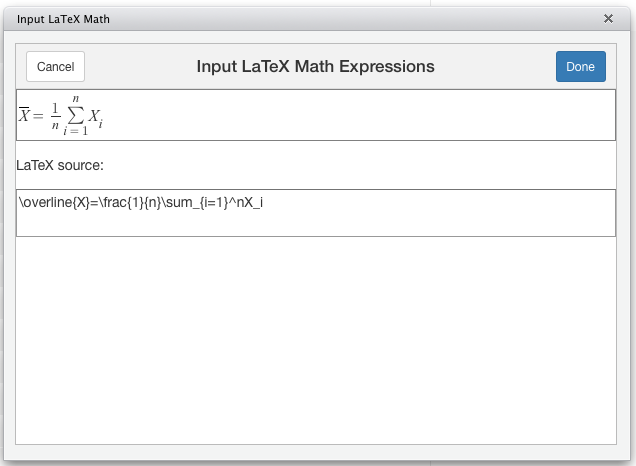
\includegraphics{images/mathquill} 

}

\caption{The RStudio addin to help input LaTeX math.}\label{fig:mathquill}
\end{figure}

There are also other R packages that provide addins to help you author books. The \textbf{citr} package \citep{R-citr} provides an addin named ``Insert citations'', which makes it easy to insert citations\index{citation} into R Markdown documents. It scans your bibliography databases, and shows all citation items in a drop-down menu, so you can choose from the list without remembering which citation key corresponds to which citation item (Figure \ref{fig:citr}).

\begin{figure}

{\centering 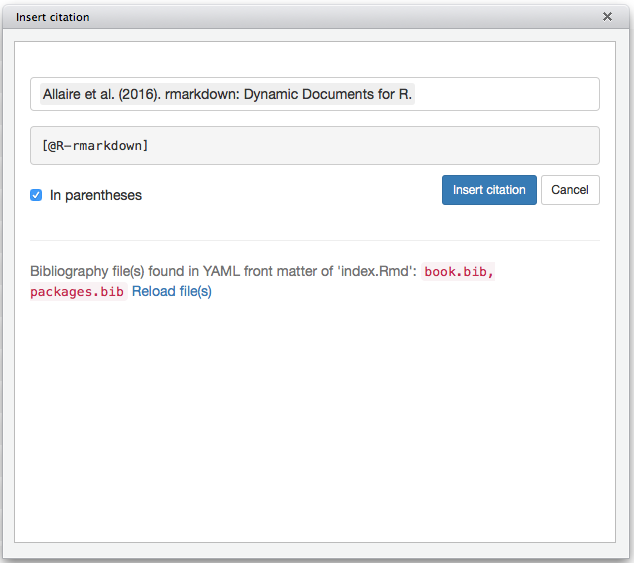
\includegraphics{images/citr} 

}

\caption{The RStudio addin to help insert citations.}\label{fig:citr}
\end{figure}

\hypertarget{collaboration}{%
\section{Collaboration}\label{collaboration}}

Writing a book will almost surely involve more than a single person. You may have co-authors, and readers who give you feedback from time to time.

Since all book chapters are plain-text files, they are perfect for version control tools, which means if all your co-authors and collaborators have basic knowledge of a version control tool like GIT, you can collaborate with them on the book content using these tools. In fact, collaboration with GIT is possible even if they do not know how to use GIT, because GitHub\index{GitHub} has made it possible to create and edit files online right in your web browser. Only one person has to be familiar with GIT, and that person can set up the book repository. The rest of the collaborators can contribute content online, although they will have more freedom if they know the basic usage of GIT to work locally.

Readers can contribute in two ways. One way is to contribute content directly, and the easiest way, is through \href{https://help.github.com/articles/about-pull-requests/}{GitHub pull requests} if your book source is hosted on GitHub. Basically, any GitHub user can click the edit button on the page of an Rmd source file, edit the content, and submit the changes to you for your approval. If you are satisfied with the changes proposed (you can clearly see what exactly was changed), you can click a ``Merge'' button to merge the changes. If you are not satisfied, you can provide your feedback in the pull request, so the reader can further revise it according to your requirements. We mentioned the edit button in the GitBook style in Section \ref{gitbook-style}. That button is linked to the Rmd source of each page, and can guide you to create the pull request. There is no need to write emails back and forth to communicate simple changes, such as fixing a typo.

Another way for readers to contribute to your book is to leave comments. Comments can be left in multiple forms: emails, GitHub issues, or HTML page comments. Here we use Disqus (see Section \ref{yaml-options}) as an example. Disqus is a service to embed a discussion area on your web pages, and can be loaded via JavaScript. You can find the JavaScript code after you register and create a new forum on Disqus, which looks like this:

\begin{Shaded}
\begin{Highlighting}[]
\KeywordTok{\textless{}div}\OtherTok{ id=}\StringTok{"disqus\_thread"}\KeywordTok{\textgreater{}\textless{}/div\textgreater{}}
\KeywordTok{\textless{}script\textgreater{}}
\NormalTok{(}\KeywordTok{function}\NormalTok{() \{ }\CommentTok{// DON\textquotesingle{}T EDIT BELOW THIS LINE}
\KeywordTok{var}\NormalTok{ d }\OperatorTok{=} \BuiltInTok{document}\OperatorTok{,}\NormalTok{ s }\OperatorTok{=}\NormalTok{ d}\OperatorTok{.}\FunctionTok{createElement}\NormalTok{(}\StringTok{\textquotesingle{}script\textquotesingle{}}\NormalTok{)}\OperatorTok{;}
\NormalTok{s}\OperatorTok{.}\AttributeTok{src} \OperatorTok{=} \StringTok{\textquotesingle{}//yihui.disqus.com/embed.js\textquotesingle{}}\OperatorTok{;}
\NormalTok{s}\OperatorTok{.}\FunctionTok{setAttribute}\NormalTok{(}\StringTok{\textquotesingle{}data{-}timestamp\textquotesingle{}}\OperatorTok{,} \OperatorTok{+}\KeywordTok{new} \BuiltInTok{Date}\NormalTok{())}\OperatorTok{;}
\NormalTok{(d}\OperatorTok{.}\AttributeTok{head} \OperatorTok{||}\NormalTok{ d}\OperatorTok{.}\AttributeTok{body}\NormalTok{)}\OperatorTok{.}\FunctionTok{appendChild}\NormalTok{(s)}\OperatorTok{;}
\NormalTok{\})()}\OperatorTok{;}
\KeywordTok{\textless{}/script\textgreater{}}
\KeywordTok{\textless{}noscript\textgreater{}}\NormalTok{Please enable JavaScript to view the}
\KeywordTok{\textless{}a}\OtherTok{ href=}\StringTok{"https://disqus.com/?ref\_noscript"}\KeywordTok{\textgreater{}}
\NormalTok{  comments powered by Disqus.}\KeywordTok{\textless{}/a\textgreater{}\textless{}/noscript\textgreater{}}
\end{Highlighting}
\end{Shaded}

Note that you will need to replace the name \texttt{yihui} with your own forum name (this name has to be provided when you create a new Disqus forum). You can save the code to an HTML file named, for example, \texttt{disqus.html}. Then you can embed it at the end of every page via the \texttt{after\_body} option (Figure \ref{fig:disqus} shows what the discussion area looks like):

\begin{Shaded}
\begin{Highlighting}[]
\PreprocessorTok{{-}{-}{-}}
\FunctionTok{output}\KeywordTok{:}
\AttributeTok{  bookdown:}\FunctionTok{:gitbook}\KeywordTok{:}
\AttributeTok{    }\FunctionTok{includes}\KeywordTok{:}
\AttributeTok{      }\FunctionTok{after\_body}\KeywordTok{:}\AttributeTok{ disqus.html}
\PreprocessorTok{{-}{-}{-}}
\end{Highlighting}
\end{Shaded}

\begin{figure}
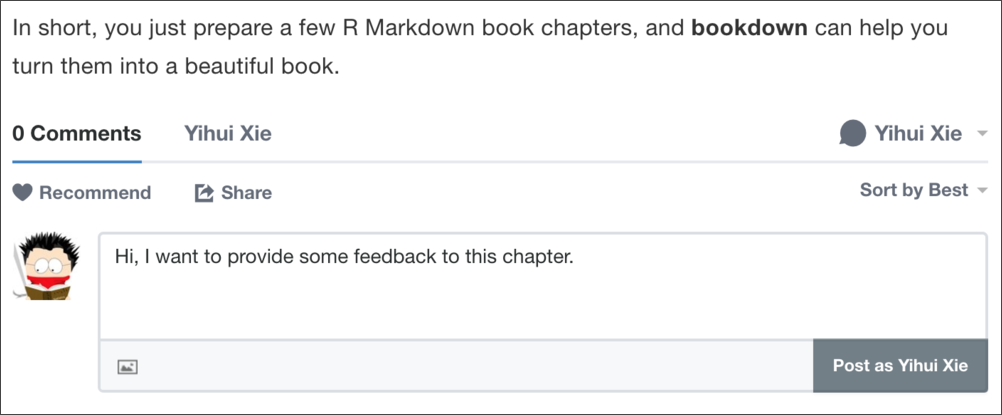
\includegraphics[width=1\linewidth]{images/disqus} \caption{A book page with a discussion area.}\label{fig:disqus}
\end{figure}

\hypertarget{ux53d1ux5e03ux4e0eux51faux7248}{%
\chapter{发布与出版}\label{ux53d1ux5e03ux4e0eux51faux7248}}

  当你在创作书籍时,你可以将书稿提供给公众,例如,将书稿发布到网站上,以便从读者那里得到早期反馈。当你完成书籍的创作后,你需要考虑正式出版书籍的方式,可以通过印刷本也可以通过电子书进行出版。

\hypertarget{rstudio-connect}{%
\section{RStudio Connect}\label{rstudio-connect}}

  理论上,你可以自己编译书籍然后将其发布到你想要的任何地方。例如,你可以在自己的 Web 服务器上托管书籍的 HTML 版本。不过我们在 \textbf{bookdown} 中提供了一个函数 \texttt{publish\_book()} ,它能够让你很轻松地将书籍上传至 \url{https://bookdown.org}。这是一个由 RStudio 提供的网站,用于免费托管你的书籍。\index{bookdown.org}这个网站建立在 \href{https://www.rstudio.com/products/connect/}{``RStudio Connect'',}\index{RStudio Connect} 之上,它是 RStudio 提供的产品之一,能够让你将各种与 R 相关的应用部署到服务器上,包括 R Markdown 文档、Shiny 应用、R plots 等。

  你不必了解太多 RStudio Connect 就能够将你的书籍发布到 bookdown.org。你需要在 \url{https://bookdown.org/connect/} 注册,之后当你第一次尝试运行 \texttt{bookdown::publish\_book()}\index{bookdown::publish\_book()} 时,系统将要求你授权 \textbf{bookdown} 发布到你的 bookdown.org 账户。以后使用时,只需要再次调用 \texttt{publish\_book()} 即可,\textbf{bookdown} 将不会要求你进行任何其他的操作。

\begin{Shaded}
\begin{Highlighting}[]
\FunctionTok{publish\_book}\NormalTok{(}\AttributeTok{name =} \ConstantTok{NULL}\NormalTok{, }\AttributeTok{account =} \ConstantTok{NULL}\NormalTok{,}
  \AttributeTok{server =} \ConstantTok{NULL}\NormalTok{, }\AttributeTok{render =} \FunctionTok{c}\NormalTok{(}\StringTok{"none"}\NormalTok{, }\StringTok{"local"}\NormalTok{, }\StringTok{"server"}\NormalTok{))}
\end{Highlighting}
\end{Shaded}

  你需要接触的 \texttt{publish\_book()} 的唯一参数是 \texttt{render}。它决定了在发布之前是否编译书籍。如果你之前已经运行过 \texttt{render\_book()},就不需要改变这个参数,否则你可能需要将其设置为 \texttt{\textquotesingle{}local\textquotesingle{}}:

\begin{Shaded}
\begin{Highlighting}[]
\NormalTok{bookdown}\SpecialCharTok{::}\FunctionTok{publish\_book}\NormalTok{(}\AttributeTok{render =} \StringTok{\textquotesingle{}local\textquotesingle{}}\NormalTok{)}
\end{Highlighting}
\end{Shaded}

  如果你已经配置好了自己的 RStudio Connect 服务器,那么当然可以将书籍发布到你自己的服务器,而不必上传至 bookdown.org。

\hypertarget{github}{%
\section{GitHub}\label{github}}

  你可以使用 GitHub Pages (\url{https://pages.github.com}) 在 GitHub\index{GitHub} 上免费托管你的书籍。GitHub 支持 Jekyll (\url{http://jekyllrb.com}), 它是一个静态网站生成器,能够将一系列 Markdown 文件转换为网站。这可能是 GitHub Pages 最常见的用法,但是 GitHub 还支持任意静态 HTML 文件,因此你可以在 GitHub 上托管书籍的 HTML 输出文件。其关键是创建一个隐藏文件 \texttt{.nojekyll},它告诉 GitHub 你的网站不是通过 Jekyll 构建的,因为 \textbf{bookdown} 的 HTML 输出文件已经是一个独立的网站。

\begin{Shaded}
\begin{Highlighting}[]
\CommentTok{\# 假设你已经初始化了一个 git 储存库,并且已经在书籍储存库的目录下}

\CommentTok{\# 创建一个隐藏文件 .nojekyll}
\FunctionTok{touch}\NormalTok{ .nojekyll}
\CommentTok{\# 将其添加入 git 版本控制中,这样她就不会再 RStudio 中显示}
\FunctionTok{git}\NormalTok{ add .nojekyll}
\end{Highlighting}
\end{Shaded}

  如果你使用 Windows,那么可能没有 \texttt{touch} 命令,这时你可以在 R 中使用 \texttt{file.create(\textquotesingle{}.nojekyll\textquotesingle{})} 来创建一个文件。

  发布书籍的一种方法将书籍的 HTML 文件放入 \texttt{master} 分支中的 \texttt{/docs} 文件夹,然后从该文件夹将书籍作为 GitHub Pagse 站点发布,就像 \href{http://bit.ly/2cvloKV}{GitHub Help}中描述的那样。首先,在配置文件 \texttt{\_bookdown.yml} 中添加一行 \texttt{output\_dir:"docs"},将书籍的输出目录设置为 \texttt{/docs}。然后,将更改推送到 GitHub ,再转到存储库的设置,在``GitHub Pages''配置项下将``Source''选项更改为``master branch/docs folder''。使用该方法时,\texttt{.nojekyll} 文件必须位于 \texttt{/docs} 文件夹中。

  另一种方法是先在存储库中创建一个 \texttt{gh-pages} 分支,再构建书籍,将 HTML 输出(包括图像、CSS 和 JavaScript 文件等所有外部资源)放入该分支,然后将该分支推送到远程存储库。如果你的书籍存储库没有 \texttt{gh-pages} 分支,可以使用以下命令创建一个分支:

\begin{Shaded}
\begin{Highlighting}[]
\CommentTok{\# 假设你已经初始化了一个 git 储存库,并且已经在书籍储存库的目录下}

\CommentTok{\# 创建一个名为 gh{-}pages 的分支,并清除全部文件}
\FunctionTok{git}\NormalTok{ checkout }\AttributeTok{{-}{-}orphan}\NormalTok{ gh{-}pages}
\FunctionTok{git}\NormalTok{ rm }\AttributeTok{{-}rf}\NormalTok{ .}

\CommentTok{\# 创建一个隐藏文件 .nojekyll}
\FunctionTok{touch}\NormalTok{ .nojekyll}
\FunctionTok{git}\NormalTok{ add .nojekyll}

\FunctionTok{git}\NormalTok{ commit }\AttributeTok{{-}m} \StringTok{"Initial commit"}
\FunctionTok{git}\NormalTok{ push origin gh{-}pages}
\end{Highlighting}
\end{Shaded}

  设置好 GIT 之后,剩下的工作可以通过脚本(Shell、R 或 Makefile,取决于你的偏好)实现自动化。总的来说,首先将书籍编译为 HTML,然后运行 git 命令将文件推送到 GitHub,但你可能不希望在本地反复手动执行这些操作,这时可以通过云来完成。由于在云上实现发布过程的完全自动化将会非常方便,因此一旦设置正确,接下来所要做的就是编写书籍并将 Rmd 源文件推送到 GitHub,你创作的书将始终在服务器端自动构建和发布。

  你可以选择使用的一个云服务是 Travis CI (\url{https://travis-ci.com})。\index{Travis CI} 它对于 GitHub 上的共有储存库提供的服务是免费的,并且是为软件包的持续集成 (CI) 而设计的。Travis CI 能够连接到 GitHub, 即每当你推送更改到 GitHub 时,Travis 能够被触发在最新版本的储存库上运行某些命令/脚本。\footnote{你需要先在 GitHub 上为你的储存库授权 Travis CI 服务。有关如何开始使用 Travis CI,请参阅 \url{https://docs.travis-ci.com/user/getting-started/}。}这些命令储存在你的储存库根目录下名为 \texttt{.travis.yml} 的 YAML 文件中。它们通常用于测试软件,但实际上它们的用途十分开放,这意味着你可以在 Travis(虚拟)机器上运行任意命令。也就是说,你当然可以在 Travis 上运行自己的脚本来构建书籍。注意,Travis 目前仅支持 Ubuntu 和 Mac OS X,因此你应该对于 Linux/Unix 命令有一些基本的了解。

  下一个问题是,怎样将在 Travis 中构建的书籍发布到 GitHub?大体上说,你需要授予 Travis 对你的 GitHub 储存库的写访问权限。该授权能够通过集中方式完成,对于初学者来说最简单的方式是个人访问令牌 (personal access token)。以下是你可以遵循的几个操作步骤:

\begin{enumerate}
\def\labelenumi{\arabic{enumi}.}
\tightlist
\item
  对于你在 GitHub 上的账户创建一个 \href{http://bit.ly/2cEBYWB}{个人访问令牌 (personal access token)}(请确保启用``repo''作用域 (``repo'' scope),以便可以通过此令牌写入你的 GitHub 储存库)。
\item
  通过命令 \texttt{travis\ encrypt} 将其加密并放在环境变量 \texttt{GITHUB\_PAT} 里,然后储存在 \texttt{.travis.yml} 文件中。例如 \texttt{travis\ encrypt\ GITHUB\_PAT=TOKEN}。如果你不知道如何安装或使用 Travis 命令行工具,只需要将这个环境变量通过 \url{https://travis-ci.com/user/repo/settings} 储存起来,其中 \texttt{user} 是你的 GitHub ID,\texttt{repo} 是储存库的名称。
\item
  你可以使用你的 GitHub 令牌在 Travis 上克隆先前创建的这个 \texttt{gh-pages} 分支,向其添加从 R Markdown 转换而来的 HTML 输出文件(不要忘记添加图片和 CSS 样式文件),然后推送到远程储存库。
\end{enumerate}

  假设你正在 \texttt{master} 分支中(你存放 Rmd 源文件的分支),并且已经编译好书籍,放在 \texttt{\_book} 目录中。接下来你可以在 Travis 中做的是:

\begin{Shaded}
\begin{Highlighting}[]
\CommentTok{\# 如果你还没有进行配置的话,设置好你的用户名和邮箱}
\FunctionTok{git}\NormalTok{ config }\AttributeTok{{-}{-}global}\NormalTok{ user.email }\StringTok{"you@example.com"}
\FunctionTok{git}\NormalTok{ config }\AttributeTok{{-}{-}global}\NormalTok{ user.name }\StringTok{"Your Name"}

\CommentTok{\# 将储存库克隆到书籍输出目录 book{-}output}
\FunctionTok{git}\NormalTok{ clone }\AttributeTok{{-}b}\NormalTok{ gh{-}pages }\DataTypeTok{\textbackslash{}}
\NormalTok{  https://}\VariableTok{$\{GITHUB\_PAT\}}\NormalTok{@github.com/}\VariableTok{$\{TRAVIS\_REPO\_SLUG\}}\NormalTok{.git }\DataTypeTok{\textbackslash{}}
\NormalTok{  book{-}output}
\BuiltInTok{cd}\NormalTok{ book{-}output}
\FunctionTok{git}\NormalTok{ rm }\AttributeTok{{-}rf} \PreprocessorTok{*}
\FunctionTok{cp} \AttributeTok{{-}r}\NormalTok{ ../\_book/}\PreprocessorTok{*}\NormalTok{ ./}
\FunctionTok{git}\NormalTok{ add }\AttributeTok{{-}{-}all} \PreprocessorTok{*}
\FunctionTok{git}\NormalTok{ commit }\AttributeTok{{-}m}\StringTok{"Update the book"}
\FunctionTok{git}\NormalTok{ push }\AttributeTok{{-}q}\NormalTok{ origin gh{-}pages}
\end{Highlighting}
\end{Shaded}

  变量名 \texttt{GITHUB\_PAT} 和目录名 \texttt{book-output} 可以是任意名称。只要名称没有与已经存在的变量名或目录名冲突,你就可以使用喜欢的任何名字。上述脚本与我们在第 \ref{build-the-book} 节提到的书籍构建脚本可以放在 \texttt{master} 分支作为 as Shell 脚本。例如,你可以将它们命名为 \texttt{\_build.sh} 和 \texttt{\_deploy.sh}。那么,你的 \texttt{.travis.yml} 文件可能是这样的:

\begin{Shaded}
\begin{Highlighting}[]
\FunctionTok{language}\KeywordTok{:}\AttributeTok{ r}
\FunctionTok{pandoc\_version}\KeywordTok{:}\AttributeTok{ }\FloatTok{1.19.2.1}

\FunctionTok{env}\KeywordTok{:}
\AttributeTok{  }\FunctionTok{global}\KeywordTok{:}
\AttributeTok{    }\KeywordTok{{-}}\AttributeTok{ }\FunctionTok{secure}\KeywordTok{:}\AttributeTok{ A\_LONG\_ENCRYPTED\_STRING}

\FunctionTok{before\_script}\KeywordTok{:}
\AttributeTok{  }\KeywordTok{{-}}\AttributeTok{ chmod +x ./\_build.sh}
\AttributeTok{  }\KeywordTok{{-}}\AttributeTok{ chmod +x ./\_deploy.sh}

\FunctionTok{script}\KeywordTok{:}
\AttributeTok{  }\KeywordTok{{-}}\AttributeTok{ ./\_build.sh}
\AttributeTok{  }\KeywordTok{{-}}\AttributeTok{ ./\_deploy.sh}
\end{Highlighting}
\end{Shaded}

  \texttt{language} 选项告诉 Travis 需要使用安装了 R 的虚拟机。\texttt{secure} 字段是加密的个人访问令牌 (personal access token )。如果你已经使用 Travis 上的 Web 界面而不是命令行工具 \texttt{travis\ encrypt} 保存了 \texttt{GITHUB\_PAT} 变量,则可以忽略这项设置。

  由于 Travis 服务主要用于检查 R 软件包,因此还需要一个(假的)\texttt{DESCRIPTION} 文件,使得书籍存储库像是一个 R 软件包一样。这个文件中唯一一个真正重要的是软件包依赖项这一配置。所有依赖项都将通过 \textbf{devtools} 包安装。如果依赖项在 CRAN 或 BioConductor 上,只需在 \texttt{DESCRIPTION} 文件的 \texttt{Imports} 字段中列出即可。如果它在 GitHub 上,您可以使用 \texttt{Remotes} 字段列出它的存储库名称。下面展示了一个例子:

\begin{verbatim}
Package: placeholder
Type: Book
Title: Does not matter.
Version: 0.0.1
Imports: bookdown, ggplot2
Remotes: rstudio/bookdown
\end{verbatim}

  如果你使用 Travis 的 \href{https://docs.travis-ci.com/user/workers/container-based-infrastructure/}{container-based infrastructure},你可以在 \texttt{.travis.yml} 中使用 \texttt{sudo:\ false} 启用缓存。通常你至少需要缓存两类目录:图片目录(例如 \texttt{\_main\_files})以及缓存目录(例如 \texttt{\_main\_cache})。如果你指定了 \textbf{knitr} 代码块选项 \texttt{fig.path} 和 \texttt{cache.path},这些目录的名称可能不同,但是我强烈建议不要改变这些设置。图片和缓存目录都存放在书籍根目录中的 \texttt{\_bookdown\_files} 目录下。启用了 \textbf{knitr} 图片和缓存的 \texttt{.travis.yml} 文件可能具有如下的 \texttt{sudo} 和 \texttt{cache} 附加配置:

\begin{Shaded}
\begin{Highlighting}[]
\FunctionTok{sudo}\KeywordTok{:}\AttributeTok{ }\CharTok{false}

\FunctionTok{cache}\KeywordTok{:}
\AttributeTok{  }\FunctionTok{packages}\KeywordTok{:}\AttributeTok{ }\CharTok{yes}
\AttributeTok{  }\FunctionTok{directories}\KeywordTok{:}
\AttributeTok{    }\KeywordTok{{-}}\AttributeTok{ $TRAVIS\_BUILD\_DIR/\_bookdown\_files}
\end{Highlighting}
\end{Shaded}

  如果构建书籍非常耗时,你可以在 Travis 上使用上面的配置来节省时间。注意,\texttt{packages:yes} 表示安装在 Travis 上的 R 包也被缓存。

  以上所有脚本和配置都可以在 \texttt{bookdown-demo} 存储库中找到:\url{https://github.com/rstudio/bookdown-demo/}。如果你将它们复制到自己的存储库中,请记住使用自己的加密变量 \texttt{GITHUB\_PAT} 更改 \texttt{.travis.yml} 文件中的 \texttt{secure} 字段。

  GitHub 和 Travis CI 当然不是构建和出版你的书籍的唯一选择。你可以在自己的服务器上自由地存储和发布这本书。

\hypertarget{ux51faux7248ux5546}{%
\section{出版商}\label{ux51faux7248ux5546}}

  除了在网上发布你的书之外,你还可以考虑通过出版商\index{publisher}出版你的书籍。例如,本书是由 Chapman \& Hall/CRC 出版的,在 \url{https://bookdown.org/yihui/bookdown/} 也有免费的在线版本(与出版商达成了协议)。如果你不想与的发布者合作,你还可以考虑自主出版 (\url{https://en.wikipedia.org/wiki/Self-publishing})。Pablo Casas 写了两篇你可能会觉得有用的博客文章:\href{https://blog.datascienceheroes.com/how-to-self-publish-a-book/}{``How to self-publish a book''} 和 \href{https://blog.datascienceheroes.com/how-to-self-publish-a-book-customizing-bookdown/}{``How to self-publish a book: customizing bookdown''}。

  如果你选择的出版商支持 LaTeX,那么出版用 \textbf{bookdown} 编写的书会容易得多。\index{LaTeX}例如,Chapman \& Hall 提供了一个名为 \texttt{krantz.cls} 的 LaTeX 类,Springer 提供的是 \texttt{svmono.cls}。如果要将这些 LaTeX 类应用于 PDF 书籍,请将 \texttt{index.Rmd} 的 YAML 元数据中的 \texttt{documentclass} 设置为 LaTeX 类文件名(不带扩展名 \texttt{.cls})。

  LaTeX 类是 YAML 元数据中最重要的设置。它控制了 PDF 书籍的整体样式。还有一些其他设置是你经常需要调整的,下面我们将展示有关本书的一些详细信息。

本书的 YAML 元数据包含以下设置:

\begin{Shaded}
\begin{Highlighting}[]
\FunctionTok{documentclass}\KeywordTok{:}\AttributeTok{ krantz}
\FunctionTok{lot}\KeywordTok{:}\AttributeTok{ }\CharTok{yes}
\FunctionTok{lof}\KeywordTok{:}\AttributeTok{ }\CharTok{yes}
\FunctionTok{fontsize}\KeywordTok{:}\AttributeTok{ 12pt}
\FunctionTok{monofont}\KeywordTok{:}\AttributeTok{ }\StringTok{"Source Code Pro"}
\FunctionTok{monofontoptions}\KeywordTok{:}\AttributeTok{ }\StringTok{"Scale=0.7"}
\end{Highlighting}
\end{Shaded}

  字段 \texttt{lot:yes} 表示我们需要表格列表;类似地,\texttt{lof} 表示图片列表。基础字体大小是 `12pt',我们使用了 \href{https://www.fontsquirrel.com/fonts/source-code-pro}{Source Code Pro} 作为等宽(固定宽度)字体,它适用于本书中的所有程序代码。

  在 LaTeX 导言 (preamble)(第 \ref{yaml-options} 节)中,我们还有一些设置。首先,我们将主字体族\index{font}设置为 \href{https://www.fontsquirrel.com/fonts/alegreya}{Alegreya},并且由于此字体没有 {Small Capitals}(小型大写字母)特征,我们使用 Alegreya SC 字体。

\begin{Shaded}
\begin{Highlighting}[]
\FunctionTok{\textbackslash{}setmainfont}\NormalTok{[}
\NormalTok{  UprightFeatures=\{SmallCapsFont=AlegreyaSC{-}Regular\}}
\NormalTok{]\{Alegreya\}}
\end{Highlighting}
\end{Shaded}

  下面的命令通过允许浮动环境\index{floating environment}占用更大部分的页面而不是浮动,从而使得它们更不太可能浮动。

\begin{Shaded}
\begin{Highlighting}[]
\FunctionTok{\textbackslash{}renewcommand}\NormalTok{\{}\ExtensionTok{\textbackslash{}textfraction}\NormalTok{\}\{0.05\}}
\FunctionTok{\textbackslash{}renewcommand}\NormalTok{\{}\ExtensionTok{\textbackslash{}topfraction}\NormalTok{\}\{0.8\}}
\FunctionTok{\textbackslash{}renewcommand}\NormalTok{\{}\ExtensionTok{\textbackslash{}bottomfraction}\NormalTok{\}\{0.8\}}
\FunctionTok{\textbackslash{}renewcommand}\NormalTok{\{}\ExtensionTok{\textbackslash{}floatpagefraction}\NormalTok{\}\{0.75\}}
\end{Highlighting}
\end{Shaded}

  由于 \texttt{krantz.cls} 为引用文段提供了一个环境 \texttt{VF},因此我们将标准的 \texttt{quote} 环境重新定义为 \texttt{VF}。您可以在第 \ref{markdown-syntax} 节中看到它的样式。

\begin{Shaded}
\begin{Highlighting}[]
\FunctionTok{\textbackslash{}renewenvironment}\NormalTok{\{quote\}\{}\KeywordTok{\textbackslash{}begin}\NormalTok{\{}\ExtensionTok{VF}\NormalTok{\}\}\{}\KeywordTok{\textbackslash{}end}\NormalTok{\{}\ExtensionTok{VF}\NormalTok{\}\}}
\end{Highlighting}
\end{Shaded}

  然后我们将超链接重新定义为脚注,因为当书印刷在纸上时,读者无法点击文本中的链接,而脚注会告诉他们实际的链接是什么。

\begin{Shaded}
\begin{Highlighting}[]
\FunctionTok{\textbackslash{}let\textbackslash{}oldhref\textbackslash{}href}
\FunctionTok{\textbackslash{}renewcommand}\NormalTok{\{}\ExtensionTok{\textbackslash{}href}\NormalTok{\}[2]\{\#2}\FunctionTok{\textbackslash{}footnote}\NormalTok{\{}\FunctionTok{\textbackslash{}url}\NormalTok{\{\#1\}\}\}}
\end{Highlighting}
\end{Shaded}

  我们还为 \texttt{\_output.yml}\index{\_output.yml} 中的 \texttt{bookdown::pdf\_book} 格式进行了一些设置:

\begin{Shaded}
\begin{Highlighting}[]
\AttributeTok{bookdown:}\FunctionTok{:pdf\_book}\KeywordTok{:}
\AttributeTok{  }\FunctionTok{includes}\KeywordTok{:}
\AttributeTok{    }\FunctionTok{in\_header}\KeywordTok{:}\AttributeTok{ latex/preamble.tex}
\AttributeTok{    }\FunctionTok{before\_body}\KeywordTok{:}\AttributeTok{ latex/before\_body.tex}
\AttributeTok{    }\FunctionTok{after\_body}\KeywordTok{:}\AttributeTok{ latex/after\_body.tex}
\AttributeTok{  }\FunctionTok{keep\_tex}\KeywordTok{:}\AttributeTok{ }\CharTok{yes}
\AttributeTok{  }\FunctionTok{dev}\KeywordTok{:}\AttributeTok{ }\StringTok{"cairo\_pdf"}
\AttributeTok{  }\FunctionTok{latex\_engine}\KeywordTok{:}\AttributeTok{ xelatex}
\AttributeTok{  }\FunctionTok{citation\_package}\KeywordTok{:}\AttributeTok{ natbib}
\AttributeTok{  }\FunctionTok{template}\KeywordTok{:}\AttributeTok{ }\CharTok{null}
\AttributeTok{  }\FunctionTok{pandoc\_args}\KeywordTok{:}\AttributeTok{ {-}{-}top{-}level{-}division=chapter}
\AttributeTok{  }\FunctionTok{toc\_unnumbered}\KeywordTok{:}\AttributeTok{ }\CharTok{no}
\AttributeTok{  }\FunctionTok{toc\_appendix}\KeywordTok{:}\AttributeTok{ }\CharTok{yes}
\AttributeTok{  }\FunctionTok{quote\_footer}\KeywordTok{:}\AttributeTok{ }\KeywordTok{[}\StringTok{"}\SpecialCharTok{\textbackslash{}\textbackslash{}}\StringTok{VA\{"}\KeywordTok{,}\AttributeTok{ }\StringTok{"\}\{\}"}\KeywordTok{]}
\AttributeTok{  }\FunctionTok{highlight\_bw}\KeywordTok{:}\AttributeTok{ }\CharTok{yes}
\end{Highlighting}
\end{Shaded}

  我们上面提到的所有导言 (preamble) 设置都在文件 \texttt{latex/preamble.tex} 中,其中我们还指定了前言 (front matter) 的开始:

\begin{quote}
译者注:\texttt{\textbackslash{}frontmatter} 通常跟在 \texttt{\textbackslash{}begin\{document\}} 后,会关闭章节序号,页码使用罗马数字。
\end{quote}

\begin{Shaded}
\begin{Highlighting}[]
\FunctionTok{\textbackslash{}frontmatter}
\end{Highlighting}
\end{Shaded}

  在 \texttt{latex/before\_body.tex} 中,我们插入了出版商要求的一些空白页,并编写了奉献页。在书的第一章之前,我们插入

\begin{Shaded}
\begin{Highlighting}[]
\FunctionTok{\textbackslash{}mainmatter}
\end{Highlighting}
\end{Shaded}

因此,LaTeX 知道将页码样式从罗马数字(前言所用的样式)更改为阿拉伯数字(正文所用的样式)。

  我们在 \texttt{latex/after\_body.tex}(第 \ref{latex-index} 节)中打印索引。

  由于默认设备 \texttt{pdf} 不能嵌入字体,因此用于保存图片的图形设备 (\texttt{dev}) 被设置为 \texttt{cairo\_pdf},以便字体可以嵌入图片中。你的文案编辑可能会要求您嵌入 PDF 中使用的所有字体,以便该书可以完全按其电子版本的外观打印,否则某些字体可能会被替换,印刷时的字型可能无法预测。

  \texttt{quote\_footer} 字段是为了确保引用页脚右对齐:\texttt{krantz.cls} 提供了 LaTeX 命令 \texttt{\textbackslash{}VA\{\}} 以包含引用页脚。

  \texttt{highlight\_bw} 选项被设置为 true,这样语法高亮显示的代码块中的颜色将转换为灰度,因为这本书将采用黑白打印。

  这本书是通过 \texttt{xelatex} 编译成 PDF 的,以便于我们使用自定义字体。

  除 \texttt{VF} 环境和 \texttt{\textbackslash{}VA\{\}} 命令外,上述所有设置都可以应用于任何其他 LaTeX 文档类。

  如果你也想与 Chapman \& Hall 合作,你可以从我们存储库 (\url{https://github.com/rstudio/bookdown/tree/master/inst/examples}) 中的 \texttt{krantz.cls} 文件开始,而不使用你从编辑那里得到的副本。我们已经与 LaTeX 帮助中心合作解决了这个 LaTeX 类的许多问题,所以如果你使用 \textbf{bookdown},希望它能很好地用于你的书。

\cleardoublepage

\hypertarget{appendix-ux9644ux5f55}{%
\appendix \addcontentsline{toc}{chapter}{\appendixname}}


\hypertarget{ux8f6fux4ef6ux5de5ux5177}{%
\chapter{软件工具}\label{ux8f6fux4ef6ux5de5ux5177}}

  对于那些不熟悉使用 R Markdown 所需的软件包的读者,我们将简要介绍这些软件包的安装和维护。

\hypertarget{r-ux548c-r-ux8f6fux4ef6ux5305}{%
\section{R 和 R 软件包}\label{r-ux548c-r-ux8f6fux4ef6ux5305}}

  R 能够从任何一个 CRAN (the Comprehensive R Archive Network) 镜像站中下载和安装,例如 \url{https://cran.rstudio.com}。请注意每年都会有一些 R 的新版本发布,你可能需要偶尔升级 R。

  为了安装 \textbf{bookdown} 阮家堡,你可以在 R 中输入:

\begin{Shaded}
\begin{Highlighting}[]
\FunctionTok{install.packages}\NormalTok{(}\StringTok{"bookdown"}\NormalTok{)}
\end{Highlighting}
\end{Shaded}

  这将安装所有必需的 R 软件包。如果你不太关心这些软件包是否实际用于编译你的书籍(例如 \textbf{htmlwidgets}),也可以选择安装所有可选的软件包:

\begin{Shaded}
\begin{Highlighting}[]
\FunctionTok{install.packages}\NormalTok{(}\StringTok{"bookdown"}\NormalTok{, }\AttributeTok{dependencies =} \ConstantTok{TRUE}\NormalTok{)}
\end{Highlighting}
\end{Shaded}

  如果想体验 GitHub 上 \textbf{bookdown} 的开发版本,需要首先安装 \textbf{devtools}:

\begin{Shaded}
\begin{Highlighting}[]
\ControlFlowTok{if}\NormalTok{ (}\SpecialCharTok{!}\FunctionTok{requireNamespace}\NormalTok{(}\StringTok{\textquotesingle{}devtools\textquotesingle{}}\NormalTok{)) }\FunctionTok{install.packages}\NormalTok{(}\StringTok{\textquotesingle{}devtools\textquotesingle{}}\NormalTok{)}
\NormalTok{devtools}\SpecialCharTok{::}\FunctionTok{install\_github}\NormalTok{(}\StringTok{\textquotesingle{}rstudio/bookdown\textquotesingle{}}\NormalTok{)}
\end{Highlighting}
\end{Shaded}

  R 软件包同样也经常在 CRAN 或 GitHub 上不断更新,因此你可能需要偶尔地更新它们:

\begin{Shaded}
\begin{Highlighting}[]
\FunctionTok{update.packages}\NormalTok{(}\AttributeTok{ask =} \ConstantTok{FALSE}\NormalTok{)}
\end{Highlighting}
\end{Shaded}

  尽管这不是必须的,但当你在处理与 R 相关的项目时,RStudio IDE 能够使很多事情变得更加简单。RStudio IDE 可以从 \url{https://www.rstudio.com} 下载。

\hypertarget{pandoc}{%
\section{Pandoc}\label{pandoc}}

  R Markdown 文档 (\texttt{*.Rmd}) 首先通过 \textbf{knitr} 软件包编译成 Markdown (\texttt{*.md}),然后通过 Pandoc 将 Markdown 编译成其他输出格式(如 LaTeX 或 HTML)。\index{Pandoc}这个过程由 \textbf{rmarkdown} 软件包自动完成。你不需要单独安装 \textbf{knitr} 或 \textbf{rmarkdown},因为它们是 \textbf{bookdown} 的必需软件包,安装 \textbf{bookdown} 时会自动安装。但是,Pandoc 不是 R 软件包,因此在安装 \textbf{bookdown} 时不会自动安装。你可以按照 Pandoc 主页 (\url{http://pandoc.org}) 上的安装说明安装 Pandoc,但是如果你使用 RStudio IDE,实际上不需要单独安装 Pandoc,因为 RStudio 包含一个 Pandoc 的副本。Pandoc 版本号可通过以下方式获得:

\begin{Shaded}
\begin{Highlighting}[]
\NormalTok{rmarkdown}\SpecialCharTok{::}\FunctionTok{pandoc\_version}\NormalTok{()}
\DocumentationTok{\#\# [1] \textquotesingle{}2.11.4\textquotesingle{}}
\end{Highlighting}
\end{Shaded}

  如果你发现这个版本太低了,并且一些 Pandoc 功能特性只在更高版本中提供,你可以安装更高版本的 Pandoc,之后 \textbf{rmarkdown} 将会调用更高版本的 Pandoc,而不是内置的版本。

\hypertarget{latex}{%
\section{LaTeX}\label{latex}}

  只有当你想要将你的书籍转为 PDF 时,你才需要 LaTeX\index{LaTeX}。你可以查阅 \url{https://www.latex-project.org/get/} 以获取更多关于 LaTeX 它的安装的信息,但是我们强烈推荐你安装名为 \href{https://yihui.org/tinytex/}{TinyTeX} 的轻量级跨平台 LaTeX 发行版,它是基于 TeX Live 构建的。TinyTeX 能够通过 R 软件包 \textbf{tinytex} 轻松安装(安装 \textbf{bookdown} 时将自动安装):

\begin{Shaded}
\begin{Highlighting}[]
\NormalTok{tinytex}\SpecialCharTok{::}\FunctionTok{install\_tinytex}\NormalTok{()}
\end{Highlighting}
\end{Shaded}

使用 TinyTeX,你将永远不会看见这样的错误信息:

\begin{Shaded}
\begin{Highlighting}[]
\NormalTok{! LaTeX Error: File \textasciigrave{}titling.sty\textquotesingle{} not found.}

\NormalTok{Type X to quit or \textless{}RETURN\textgreater{} to proceed,}
\NormalTok{or enter new name. (Default extension: sty)}

\NormalTok{Enter file name: }
\NormalTok{! Emergency stop.}
\NormalTok{\textless{}read *\textgreater{} }
         
\NormalTok{l.107 \^{}\^{}M}

\NormalTok{pandoc: Error producing PDF}
\NormalTok{Error: pandoc document conversion failed with error 43}
\NormalTok{Execution halted}
\end{Highlighting}
\end{Shaded}

  上面的错误信息表示你使用了一个包含 \texttt{titling.sty} 的 LaTeX 软件包,但它并没有被安装。LaTeX 软件包名称通常是 \texttt{*.sty} 这样的文件名格式,因此在本例中,你可以尝试安装 \texttt{titling} 软件包。如果你使用带有 R Markdown 的 TinyTeX,丢失的 LaTeX 软件包将自动安装,因此你无需担心此类问题。

  LaTeX 发行版和其软件包也不时会进行更新,你可以考虑更新它们,特别是当您遇到 LaTeX 问题时。你可以通过以下方式找到 LaTeX 发行版的版本:

\begin{Shaded}
\begin{Highlighting}[]
\FunctionTok{system}\NormalTok{(}\StringTok{\textquotesingle{}pdflatex {-}{-}version\textquotesingle{}}\NormalTok{)}
\DocumentationTok{\#\# pdfTeX 3.141592653{-}2.6{-}1.40.23 (TeX Live 2021/W32TeX)}
\DocumentationTok{\#\# kpathsea version 6.3.3}
\DocumentationTok{\#\# Copyright 2021 Han The Thanh (pdfTeX) et al.}
\DocumentationTok{\#\# There is NO warranty.  Redistribution of this software is}
\DocumentationTok{\#\# covered by the terms of both the pdfTeX copyright and}
\DocumentationTok{\#\# the Lesser GNU General Public License.}
\DocumentationTok{\#\# For more information about these matters, see the file}
\DocumentationTok{\#\# named COPYING and the pdfTeX source.}
\DocumentationTok{\#\# Primary author of pdfTeX: Han The Thanh (pdfTeX) et al.}
\DocumentationTok{\#\# Compiled with libpng 1.6.37; using libpng 1.6.37}
\DocumentationTok{\#\# Compiled with zlib 1.2.11; using zlib 1.2.11}
\DocumentationTok{\#\# Compiled with xpdf version 4.03}
\end{Highlighting}
\end{Shaded}

  你可以运行如下代码来更新 TinyTeX:

\begin{Shaded}
\begin{Highlighting}[]
\NormalTok{tinytex}\SpecialCharTok{::}\FunctionTok{tlmgr\_update}\NormalTok{()}
\end{Highlighting}
\end{Shaded}

  随着时间的推移,你可能也需要升级 TinyTeX(否则你无法安装或更新任何 LaTeX 软件包),在这种情况下你需要重新安装 TinyTeX:

\begin{Shaded}
\begin{Highlighting}[]
\NormalTok{tinytex}\SpecialCharTok{::}\FunctionTok{reinstall\_tinytex}\NormalTok{()}
\end{Highlighting}
\end{Shaded}

\hypertarget{ux8f6fux4ef6ux4f7fux7528}{%
\chapter{软件使用}\label{ux8f6fux4ef6ux4f7fux7528}}

  如第 \ref{introduction} 章所述,这本书并不是一本全面的 \textbf{knitr} 或 \textbf{rmarkdown} 指南。在本章中,我们简要地解释了 \textbf{knitr} 和 \textbf{rmarkdown} 中的一些基本概念和语法。如果你还有什么问题,可以将它们发布到 StackOverflow (\url{https://stackoverflow.com}) 上,并用 \texttt{r}、\texttt{knitr}、\texttt{rmarkdown} 和/或 \texttt{bookdown} 等任何适合的标签标记你的问题。

\hypertarget{knitr}{%
\section{knitr}\label{knitr}}

  \textbf{knitr} 软件包\index{knitr}是基于``文学编程''\citep{knuth1984}的思想设计的,它允许你将程序代码与源文档中的文本混合在一起。当 \textbf{knitr} 编译文档时,将提取并执行程序代码(以代码块为单位),程序输出将与输出文档中的原始文本一起显示。我们在第 \ref{r-code} 节中介绍了基本的语法。

  R Markdown 不是 \textbf{knitr} 支持的唯一源格式。\textbf{knitr} 的基本思想可应用于其他计算和创作语言。例如,\textbf{knitr}还支持 R 和 LaTeX 的组合(\texttt{*.rnw}文档),以及 R + HTML (\texttt{*.RtML}) 等。你也可以在 \textbf{knitr} 中 使用其他计算语言,如 C++、Python、SQL 等。下面是一个简单的例子,你可以在 \url{http://rmarkdown.rstudio.com/authoring_knitr_engines.html} 中了解更多信息。

\begin{Shaded}
\begin{Highlighting}[]
\InformationTok{\textasciigrave{}\textasciigrave{}\textasciigrave{}\{python\}}
\InformationTok{x = \textquotesingle{}Hello, Python World!\textquotesingle{}}
\InformationTok{print(x.split(\textquotesingle{} \textquotesingle{}))}
\InformationTok{\textasciigrave{}\textasciigrave{}\textasciigrave{}}
\end{Highlighting}
\end{Shaded}

  Python 用户可能熟悉 IPython\index{IPython} 或 Jupyter\index{Jupyter Notebook} Notebooks (\url{https://jupyter.org})。事实上,R Markdown 也可以作为笔记本使用,并有一些额外的优势;有关这方面详细信息,请参阅这篇博客文章:\url{https://blog.rstudio.org/2016/10/05/r-notebooks/}。

  如果要在文档中显示文本形式的代码块,可以在块头部之前添加一个内联表达式,该表达式生成一个空字符串 (\texttt{\textasciigrave{}r\ \textquotesingle{}\textquotesingle{}\textasciigrave{}}),并将代码块用在四个反引号包裹起来,\footnote{如果要在列表等其他环境中显示文字形式的代码块,请遵循缩进规则:\url{https://pandoc.org/MANUAL.html\#block-content-in-list-items}},例如:

\begin{Shaded}
\begin{Highlighting}[]
\InformationTok{\textasciigrave{}\textasciigrave{}\textasciigrave{}\textasciigrave{}}
\InformationTok{\textasciigrave{}r \textquotesingle{}\textquotesingle{}\textasciigrave{}\textasciigrave{}\textasciigrave{}\textasciigrave{}\{r\}}
\InformationTok{\# a literal code chunk}
\InformationTok{\textasciigrave{}\textasciigrave{}\textasciigrave{}}
\InformationTok{\textasciigrave{}\textasciigrave{}\textasciigrave{}\textasciigrave{}}
\end{Highlighting}
\end{Shaded}

  当文档被编译后,内联表达式将会消失,你会看到:

\begin{Shaded}
\begin{Highlighting}[]
\InformationTok{\textasciigrave{}\textasciigrave{}\textasciigrave{}\{r\}}
\InformationTok{\# a literal code chunk}
\InformationTok{\textasciigrave{}\textasciigrave{}\textasciigrave{}}
\end{Highlighting}
\end{Shaded}

  编译文档时通常不需要直接调用 \textbf{knitr} 函数,因为 \textbf{rmarkdown} 会调用 \textbf{knitr}。如果你希望编译源文档而不进一步将其转换为其他格式,可以使用 \texttt{knitr::knit()} 函数。

\hypertarget{r-markdown}{%
\section{R Markdown}\label{r-markdown}}

  由于 R 和 Pandoc 的强大功能,你可以轻松地在 R Markdown 文档中进行计算,并将其转换为各种输出格式,包括 HTML/PDF/Word 文档、HTML5/Beamer 幻灯片、仪表板和网站等。R Markdown 文档通常由 YAML\index{YAML} 元数据(可选)和文档主体组成。我们在第 \ref{components} 章中介绍了编写文档主体各个组件的语法,并在本节中详细解释了 YAML 元数据。

  R Markdown 的元数据可以写在文档的最开头,分别以三个短划线 \texttt{-\/-\/-} 开头和结尾。YAML 元数据通常由冒号分隔的标记值对组成,例如:

\begin{Shaded}
\begin{Highlighting}[]
\PreprocessorTok{{-}{-}{-}}
\FunctionTok{title}\KeywordTok{:}\AttributeTok{ }\StringTok{"An R Markdown Document"}
\FunctionTok{author}\KeywordTok{:}\AttributeTok{ }\StringTok{"Yihui Xie"}
\PreprocessorTok{{-}{-}{-}}
\end{Highlighting}
\end{Shaded}

For character values, you may omit the quotes when the values do not contain special characters, but it is safer to quote them if they are expected to be character values.

Besides characters, another common type of values are logical values. Both \texttt{yes} and \texttt{true} mean true, and \texttt{no}/\texttt{false} mean false, e.g.,

\begin{Shaded}
\begin{Highlighting}[]
\FunctionTok{link{-}citations}\KeywordTok{:}\AttributeTok{ }\CharTok{yes}
\end{Highlighting}
\end{Shaded}

Values can be vectors, and there are two ways of writing vectors. The following two ways are equivalent:

\begin{Shaded}
\begin{Highlighting}[]
\FunctionTok{output}\KeywordTok{:}\AttributeTok{ }\KeywordTok{[}\StringTok{"html\_document"}\KeywordTok{,}\AttributeTok{ }\StringTok{"word\_document"}\KeywordTok{]}
\end{Highlighting}
\end{Shaded}

\begin{Shaded}
\begin{Highlighting}[]
\FunctionTok{output}\KeywordTok{:}
\AttributeTok{  }\KeywordTok{{-}}\AttributeTok{ }\StringTok{"html\_document"}
\AttributeTok{  }\KeywordTok{{-}}\AttributeTok{ }\StringTok{"word\_document"}
\end{Highlighting}
\end{Shaded}

Values can also be lists of values. You just need to indent the values by two more spaces, e.g.,

\begin{Shaded}
\begin{Highlighting}[]
\FunctionTok{output}\KeywordTok{:}
\AttributeTok{  bookdown:}\FunctionTok{:gitbook}\KeywordTok{:}
\AttributeTok{    }\FunctionTok{split\_by}\KeywordTok{:}\AttributeTok{ }\StringTok{"section"}
\AttributeTok{    }\FunctionTok{split\_bib}\KeywordTok{:}\AttributeTok{ }\CharTok{no}
\end{Highlighting}
\end{Shaded}

It is a common mistake to forget to indent the values. For example, the following data

\begin{Shaded}
\begin{Highlighting}[]
\FunctionTok{output}\KeywordTok{:}
\FunctionTok{html\_document}\KeywordTok{:}
\FunctionTok{toc}\KeywordTok{:}\AttributeTok{ }\CharTok{yes}
\end{Highlighting}
\end{Shaded}

actually means

\begin{Shaded}
\begin{Highlighting}[]
\FunctionTok{output}\KeywordTok{:}\AttributeTok{ }\CharTok{null}
\FunctionTok{html\_document}\KeywordTok{:}\AttributeTok{ }\CharTok{null}
\FunctionTok{toc}\KeywordTok{:}\AttributeTok{ }\CharTok{yes}
\end{Highlighting}
\end{Shaded}

instead of what you probably would have expected:

\begin{Shaded}
\begin{Highlighting}[]
\FunctionTok{output}\KeywordTok{:}
\AttributeTok{  }\FunctionTok{html\_document}\KeywordTok{:}
\AttributeTok{    }\FunctionTok{toc}\KeywordTok{:}\AttributeTok{ }\CharTok{yes}
\end{Highlighting}
\end{Shaded}

The R Markdown output format is specified in the \texttt{output} field of the YAML metadata, and you need to consult the R help pages for the possible options, e.g., \texttt{?rmarkdown::html\_document}, or \texttt{?bookdown::gitbook}. The meanings of most other fields in YAML can be found in the Pandoc documentation.

The \textbf{rmarkdown} package has provided these R Markdown output formats:

\begin{itemize}
\tightlist
\item
  \texttt{beamer\_presentation}
\item
  \texttt{context\_document}
\item
  \texttt{github\_document}
\item
  \texttt{html\_document}
\item
  \texttt{ioslides\_presentation}
\item
  \texttt{latex\_document}
\item
  \texttt{md\_document}
\item
  \texttt{odt\_document}
\item
  \texttt{pdf\_document}
\item
  \texttt{powerpoint\_presentation}
\item
  \texttt{rtf\_document}
\item
  \texttt{slidy\_presentation}
\item
  \texttt{word\_document}
\end{itemize}

There are many more possible output formats in other R packages, including \textbf{bookdown}, \textbf{tufte}, \textbf{rticles}, \textbf{flexdashboard}, \textbf{revealjs}, and \textbf{rmdformats}, etc.

\hypertarget{ux5e38ux89c1ux95eeux9898}{%
\chapter{常见问题}\label{ux5e38ux89c1ux95eeux9898}}

  下面是常见问题 (FAQ) 的\emph{完整}列表。是的,这里只有一个问题。我个人不喜欢 FAQs。它们通常意味着惊喜,而惊喜对软件用户来说并不好。

\begin{enumerate}
\def\labelenumi{\arabic{enumi}.}
\item
  问:\textbf{bookdown} 会不会有 X、Y 和 Z功能?

  答:简而言之,答案是否定的。但是如果你已经问了自己多次``我真的需要这些功能吗'',而答案仍然是``是''时,请随时向我们提出功能要求 \url{https://github.com/rstudio/bookdown/issues}。

  用户要求的更多功能往往来自 LaTeX 世界。如果你的功能要求是这样的话,这个问题的答案是肯定的,因为 Pandoc 的 Markdown 支持原始 LaTeX 代码。每当你觉得 Markdown 不能为你完成这项工作时,总是可以选择在 Markdown 文档中应用一些原始的 LaTeX 代码。例如,你可以使用 \textbf{glossaries} 软件包创建术语表,或者你知道 LaTeX 语法的话,可以嵌入一个复杂的 LaTeX 表。但是请记住,LaTeX 内容不可移植。它只适用于 LaTeX/PDF 输出,在其他类型的输出中将被忽略。根据要求,我们将来可能会在 \textbf{bookdown} 中引入更多的 LaTeX 功能,但我们的基本理念是 Markdown 应该尽可能简单。
\end{enumerate}

  世界上最具挑战性的不是学习花哨的技术,而是控制自己的狂野之心。

\backmatter

  \bibliography{book.bib,packages.bib}

\printindex

\end{document}
